%% Verze pro oboustranny tisk:
% Okraje: 
% (ale pozor, LaTeX si prida 1in)
\documentclass[12pt,a4paper,twoside]{book}
\usepackage[czech,english]{babel}
\setlength\textwidth{155mm}
\setlength\textheight{242mm}
\setlength\oddsidemargin{5mm}
\setlength\evensidemargin{-5mm}
\setlength\topmargin{0mm}
%\setlength\headheight{15mm}
\setlength{\headheight}{15pt}
%\setlength{\parindent}{1cm}
\usepackage{pdfpages}
\usepackage{textcomp}

\usepackage[utf8]{inputenc}

\usepackage{bibentry}
\usepackage{url}
\usepackage[nottoc]{tocbibind}
\nobibliography*

\usepackage{titlesec}  %vzhled titulku prvni stranky kapitoly
%\let\footruleskip\undefined
\usepackage{fancyhdr}  %hlavicky stranek 

%% Ostatn� bal��ky
\usepackage{graphicx}
%\usepackage{amsthm} % for mathematical theorems, lemma, proof
\usepackage{amsmath} % for mathematical equation
\usepackage{amssymb} % for special symbols - blacktriangledown
%\usepackage{palatino} % font
%\usepackage{bookman} % another font
\usepackage[sc]{mathpazo} %palladio font
\usepackage[scaled]{helvet}
\usepackage{eulervm}

\usepackage{setspace} % for linespacing
%\linespread{1.0}%\sin­glespac­ing %\onehalfspacing 
\usepackage[T1]{fontenc} %font encoding e.g. for czech characters
\usepackage{diagbox} %diagonala v tabulce
\usepackage{multirow} %viceradkove tabulky
\usepackage[font=footnotesize]{caption} %velikost fontu v popisu
\usepackage{etoolbox} %pro pozdejsi definici zpetne reference
\usepackage[titletoc]{appendix} %appendices with names
\usepackage{listings,multicol} % for code listings, multicolumned
\lstset{% escape sequence inside listing
  escapeinside={(*}{*)},%
}
\usepackage{dtsyntax} % for listings modelica
\usepackage[version=3]{mhchem} % for writing chemical compounds and reaction
\usepackage{siunitx} % formating numbers
\usepackage[intoc,refpage]{nomencl} % list of abbreviation

\makenomenclature
\renewcommand{\nomname}{List of Abbreviation}

\renewcommand{\ttdefault}{pcr} % nicer font - courier in listing
\usepackage[unicode,colorlinks,backref=page]{hyperref}   % Musi byt za vsemi ostatnimi balicky
\hypersetup{pdftitle={Utilization of GRID in processing of medical information},
            pdfauthor={Tomáš Kulhánek},
            plainpages=false,
            urlcolor=blue,
            linkcolor=blue,
            citecolor=blue
            }

%\overfullrule=2cm %vyznacit na okraji, kde se nepodarilo zarovnat
%definice jak ma vypadat zpetna reference
\makeatletter
\patchcmd{\BR@backref}{\newblock}{\newblock(cited on p.~}{}{}
\patchcmd{\BR@backref}{\par}{)\par}{}{}
\renewcommand\bibentry[1]{\nocite{#1}{\frenchspacing
     \@nameuse{BR@r@#1\@extra@b@citeb}}}
\makeatother


\begin{document}
\shorthandoff{-} % fix problems with babel czech and includepdf chars '-' 
\pagenumbering{roman} %first pages with roman numbering
\setcounter{page}{1}
\lefthyphenmin=2
\righthyphenmin=2
\pagestyle{empty} % title page without number
\singlespacing 
%\sin­glespac­ing % 1.0 row space
\begin{center}
%\singlespacing 
\large
%\begin{tabular}{rl}
\textbf{\Large{Univerzita Karlova v Praze}}

\textbf{\Large{1.lékařská fakulta}} 

\textit{Charles University in Prague} 

\textit{1st Faculty of Medicine}
%\end{tabular}
\vfill
\normalsize
\begin{tabular}{rl}
Studijní obor:  & Biomedicínská informatika \\
\noalign{\vspace{-1mm}}
\textit{Study domain} & \textit{Biomedical informatics} \\
\end{tabular}

\vfill

\vspace{10mm}

\centerline{\mbox{
\includegraphics[width=65mm]{img/logouk.jpg}

\includegraphics[width=65mm]{img/logolf1.jpg}}}

\vfill
\vspace{10mm}

{\Large Mgr. Tomáš Kulhánek}

\vspace{8mm}

% N�zev pr�ce p�esn� podle zad�n�
\textbf{\large Využití technologie GRID při zpracování medicínské informace}

\vspace{2mm}
\textit{\large Utilization of GRID technology in processing of medical information}

\vfill

% N�zev katedry nebo �stavu, kde byla pr�ce ofici�ln� zad�na
% (dle Organiza�n� struktury MFF UK)
% CESNET z.s.p.o., Institute of pathological physiology


{\Large Dizertační práce}

\textit{\large Dissertation}

\vfill


\begin{tabular}{rl}

Školitel: & Ing. Milan Šárek, CSc. \\
\noalign{\vspace{-1mm}}
\textit{Supervisor} \\
\noalign{\vspace{2mm}}
Konzultant: & Doc. MUDr. Jiří Kofránek, CSc. \\
\noalign{\vspace{-1mm}}
\textit{Consultant} \\
\noalign{\vspace{2mm}}
\end{tabular}

\vfill

Praha 2015

\end{center}
\newpage
\mbox{}

%\frontmatter
\onehalfspacing %1.5 row space

\newpage
\vglue 0pt plus 1fill
\selectlanguage{czech}
%\normalsize
\noindent\Large \textbf{Prohlášení}

\normalsize
\noindent Prohlašuji, že jsem závěrečnou práci zpracoval samostatně a že jsem řádně uvedl a citoval všechny použité prameny a literaturu. Současně prohlašuji, že práce nebyla využita k získání jiného nebo stejného titulu.

\vspace{5mm}
\noindent Souhlasím s trvalým uložením elektronické verze mé práce v databázi systému meziuniverzitního projektu Theses.cz za účelem soustavné kontroly podobnosti kvalifikačních prací.


\vspace{15mm}

V Praze, 2015 \hfill          Mgr. Tomáš Kulhánek
\vspace{10mm}
					
\hfill Podpis

\vspace{20mm}

\newpage
\mbox{}
\newpage
\noindent\Large\textbf{Identifikační záznam}

\normalsize
\noindent
KULHÁNEK, Tomáš. \emph{Využití technologie GRID při zpracování medicínské informace}. Dizertační práce. Praha, 2015. 44 stran. 7 příloh. Univerzita Karlova v Praze, 1. lékařská fakulta, Ústav patologické fyziologie. Školitel Šárek, Milan. Konzultant Kofránek, Jiří.

\vspace{10mm}

\noindent\Large\textbf{Identification record}

\normalsize
\noindent
KULHÁNEK, Tomáš. \emph{Utilization of GRID technology in processing of medical information}. Dissertation. Prague, 2015. 44 pages. 7 appendices. Charles University in Prague, 1st Faculty of Medicine, Institute of Pathological Physiology. Supervisor Šárek, Milan. Consultant Kofránek, Jiří.

\newpage
\mbox{}


%\onehalfspacing


\newpage
\selectlanguage{english}

\begin{center}
\Large \textbf{Dedication}
\end{center} 
\vfill
\begin{center}
To my beloved children Karla and Matěj and my dearest lovely wife Marie,

without whom this work would not have been completed.
\end{center} 
\vfill
\newpage
\mbox{}
\newpage
\pagestyle{plain} % other pages with number
\begin{center}
\Large \textbf{Acknowledgements}
\end{center} 
I would like to express my gratefulness to my supervisor Ing. Milan Šárek, CSc. for his support and guidance throughout the beginning of my research. 
I would also like to thank the staff of association CESNET, especially Ing. Jiří Navrátil, CSc., who gave me an opportunity to work with computing resources connected via high speed academic network and to follow the development of the networking technologies. Further thanks go to the staff of METACENTRUM, department of CESNET, for giving support and access to powerful computing infrastructure for scientific purposes. I would like to thank to the staff of EGI.eu, who gave me an opportunity to be EGI Champion, selected users of scientific European grid-computing and cloud-computing infrastructure. This made me possible to meet the most inspiring people in the technology domain as well as scientific domain face to face. 

I would like to thank the fellows from Musical Acoustic Research Center of Academy of Performing Arts, especially RNDr. Marek Frič, PhD. and Ing. Zdeněk Otčenášek, Phd. for their inspiring atmosphere in the research domain of voice science. 

I would like to thank my colleagues from Laboratory of Biocybernetics and Computer Aided Teaching within Institute of Pathological Physiology including Mgr. Marek Mateják, Ing. Jan Šilar, Ing. Filip Ježek, Ing. Martin Tribula and MUDr. et Mgr. Pavol Privitzer, who provided me pleasure and inspiring atmosphere for my research and development work during the second part of my research. Especially, I would like to thank to my consultant Doc. MUDr. Jiří Kofránek, CSc. and a fellow MUDr. Stanislav Matoušek, PhD., who taught me the subject of medical physiology and who guided me within the topic of mathematical models and simulation of integrative physiology. Last but not least, thanks to Veronika Sýkorová, DiS and Klára Ulčová, DiS for their help with graphical schemas. 

The research projects were solved within the cooperation between association CESNET, First Faculty of Medicine of Charles University in Prague and Academy of Performing Arts in Prague and was partially supported by the project of Ministry of Education, Youth and Sport of the Czech Republic MSM6383917201, by the projects of Development Fund of CESNET 2009/361, 2010/384, 2011/423, 2011/431 and by the project of Ministry of Industry and Trade of the Czech Republic MPO FR-TI3/869.

\newpage
\mbox{}

\pagestyle{plain} % other pages with number

%%% Povinn� informa�n� strana diserta�n� pr�ce

\vbox to 0.5\vsize{
\begin{center}
\Large \textbf{Abstrakt (česky)}
\end{center} 
\normalsize
\setlength\parindent{0mm}
\setlength\parskip{2mm}
\selectlanguage{czech}
\textbf{Název práce:}
Využití technologie GRID při zpracování medicínské informace

\textbf{Autor:}
Mgr. Tomáš Kulhánek

\textbf{Katedra,ústav: }
Ústav patologické fyziologie 1.LFUK  

\textbf{Školitel:}
Ing. Milan Šárek, CSc., CESNET z.s.p.o.

\textbf{Konzultant:}
Doc. MUDr. Jiří Kofránek, CSc.

Práce se soustředí na vybrané oblasti biomedicínského výzkumu, které mohou profitovat ze současných výpočetních infrastruktur vybudovaných ve vědecké komunitě v evropském a světovém prostoru. Teorie výpočtu, paralelismu a distribuovaného počítání je stručně uvedena s ohledem na počítání v gridech a cloudech. Byla studována oblast výměny medicínských snímků a Gridový PACS systém byl propojen s existujícími distribuovanými systémy pro sdílení DICOM snímků. Další studovanou doménou byla věda týkající se lidského hlasu. Vzdálený přístup k aplikaci pro analýzu hlasu v reálném čase byl představen zároveň s úpravou protokolů pro vzdálenou plochu pro přenos zvukových nahrávek. To přináší možnost využití stávajících aplikací na dálku specialisty na hlas. 

Byl studován přístup tzv. systémové biologie v oblasti lidské fyziologie a patofyziologie. Bylo přispěno k metodologii modelování lidské fyziologie pro tvorbu komplexních modelů založených na akauzálním a objektově orientovaném modelovacím přístupu. Byly představeny metody pro studium parametrů pomocí technologie počítání v gridech a v cloudech. Proces identifikace parametrů středně komplexních modelů kardiovasculárního systému a komplexního modelu lidské fyziologie lze významně zrychlit při použití cloud computingu a dobrých výsledků lze dosáhnout v rozumném čase. Tato metoda umožňuje aplikovat parametrické studie ve fyziologickém a biologickém výzkumu. Toto může zlepšit praktické použití matematických modelů a identifikaci parametrů ve zdravotní péči.

%This thesis focuses on selected areas of biomedical research in order to benefit from current computational infrastructures established in scientific community in european and global area. The theory of computation, parallelism and distributed computing, with focus on grid computing and cloud computing, is briefly introduced. A seamless integration of grid-based PACS system was established with the current distributed system in order to share DICOM medical images. Access to real-time voice analysis application via remote desktop technology brings this type of service to any computer that can connect to the Internet. 
%%A system and portal was introduced in order to estimate the parameters of the model and perform parameter study. Additionally, 
%The modeling methodology was contributed in order to build complex models based on  acausal and object-oriented modeling techniques. Methods for conducting a parameter study were shown, especially parameter estimation and parameter sweep. Parameter study of complex models gain substantial speedup by utilizing cloud computing deployment, which makes such kinds of complex studies applicable in physiological and biological research and have potential to improve such usage in healthcare.
%%support parameter estimation and parameter sweep. 
%
%The multidisciplinary projects were solved within the cooperation between association CESNET, First Faculty of Medicine of Charles University in Prague and Academy of Performing Arts in Prague. The work was partially supported by the project of Ministry of Education, Youth and Sport of the Czech Republic MSM6383917201, by the projects of Development Fund of CESNET 2009/361, 2010/384, 2011/423 and 2011/431 and by the project of Ministry of Industry and Business of the Czech Republic MPO FR-TI3/869.




%Práce prezentuje výzkum a výsledky využití technologií, které umožňují sdílet výpočetní a úložné kapacity a to v oblasti biomedicínského výzkumu. Vedle technologie GRID se rozvíjí virtualizačních technologie (VMWare, XEN, ...), které dodali distribuovaným systémům novou vlastnost zdání vlastnictví a přímé kontroly konfigurovatelné infrastruktury jako služby, jež se dnes shrnují pod společný pojem CLOUD computing. V práci jsou diskutovány teoretické limity distribuovaných systémů a paralelních výpočtů v nich tak i praktické výsledky ve vybraných oblastech. V oblasti výměny medicínských snímků a souvisejících zdravotních záznamů byla ukázána snadná integrovatelnost se stávajícími systémy při respektování požadavků na bezpečnost dat. V oblasti analýzy a zpracování lidského hlasu v reálném čase byla ukázána možnost poskytování nadstandardních výpočetních služeb pro komunitu uživatelů. V oblasti modelování fyziologických systémů je prezentován systém pro odhad parametrů a identifikaci fyziologických systémů komplexních modelů, které by byli obtížně řešitelné za použití klasických metod.

\textbf{Klíčová slova:}
gridové počítání, počítání v cloudu, výpočetní fyziologie, systémová biologie, odhad parametrů, výměna medicínských snímků, analýza hlasového signálu
\vss}

\newpage

\nobreak\vbox to 0.49\vsize{
\setlength\parindent{0mm}
\setlength\parskip{5mm}
\selectlanguage{english}
\textbf{Title:}
Utilization of GRID technology in processing medical information

\textbf{Author:}
Tomáš Kulhánek

\textbf{Department:}
Institute of pathological Physiology

\textbf{Supervisor:}
Ing. Milan Šárek, CSc., CESNET z.s.p.o

\textbf{Consultant:}
Doc. MUDr. Jiří Kofránek, CSc.

\textbf{Abstract:}

Two work presents results, which are researched in the field of utilization technology who offers distributed computing and storage capacity to exchange medical information, demanding computation and data exchange. Next to the GRID technology. The virtualization technology evolved and were utilized more massively next to the GRID technology and these gives distributed systems a new quality and services called today with the name CLOUD. This work summarizes result of different projects which implements selected technologies in the field of GRID and CLOUD to systems which are used in medical education and research and in neighboring fields. The multidisciplinary projects were solved within the cooperation between association CESNET, First Faculty of Medicine of Charles University in Prague and Academy of Performing Arts in Prague.

% abstrakt v rozsahu 80-200 slov v angli�tin�; nejedn� se v�ak o p�eklad
% zad�n� diserta�n� pr�ce

\textbf{Keywords:}
grid, cloud, computational physiology, phonetogram
% 3 a� 5 kl��ov�ch slov v angli�tin�

\vss}

\small

\tableofcontents

\mainmatter

\pagenumbering{arabic} %thesis pages with arabic numering
\setcounter{page}{1}

%\pagestyle{fancy}
%\fancyfoot[LE,RO]{\thepage}
\pagestyle{fancyplain}
\fancyhf{}
%\lhead{ \fancyplain{}{\leftmark} }
\fancyhead[LE]{ \fancyplain{}{\leftmark} }
%\fancyhead[RE]{ \thepage }
\fancyhead[RO]{ \fancyplain{}{\leftmark} }
%\fancyhead[LO]{ \thepage }

\cfoot{ \thepage }

%\lhead{}
%\cfoot{}
%\fancyhead[LE,RO]{\thepage}
%\fancyhead[LE,RO]{\slshape \rightmark}
%\fancyhead[LO,RE]{\slshape \leftmark}

\chapter{Introduction}

The \emph{grid-computing} is usually defined as sharing computational and data storage resources across organizational boundaries. In recent years, the development of virtualization technologies enhances the availability of services provided by grid-computing and additionally enabled an evolution of so called \emph{cloud-computing}, which can utilize virtual environment on real powerful computing infrastructure too. Based on the development of technologies and also philosophy of providing them to end users, this thesis focus on multidisciplinary research related to grid-computing as well as to cloud-computing and it's utilization in biomedical research and application related to processing of medical information.

The term "medical information" is too wide and further work focuses on the following selected areas, which were part of:
(1) exchange and processing of medical images, (2) analysis of human voice and (3) modeling and simulation of human physiology. %This work focuses on processing of medical information should give enhanced information, which can be analysed easily. Thus further analysis or synthesis of such information is beyond this work, so the aim is not to give particular results on some specific diseasies, pathologies etc., however, with cooperation of other experts it is a desired side effect.

The author's work was published in a series of peer-reviewed papers of international journals and peer-reviewed conference proceedings \cite{kulhanek2009, kulhanek2010b, kulhanek2010c,  
Kulhanek2014Parameters, Kulhanek2014Modeling, Kulhanek2014mefanet, Matejak2014sj} which are attached into this work as appendices.
The author's work and contribution was also presented in international conferences and published in the respective proceedings and transactions
\cite{Kulhanek2010, Kulhanek2013c, kofranek2013hummod, Matejak2014}. The work was also popularized on the local and regional conferences and their respective proceedings \cite{Kulhanek2008Mefanet, Sarek2009, kulhanek2009dd, Kulhanek2009Mefanet, Kulhanek2010d, Kulhanek2010Mefanet, Kulhanek2011, kulhanek2011dd, Kulhanek2012, Kulhanek2013b, Kulhanek2014, Kulhanek2012a}. Author contributed to the utility model registered by the Czech Industrial Property Office \cite{Kofranek2014a}.

\section{Thesis Goal}
\label{sec:goal}
The hypothesis stated by this thesis is that the technologies related to grid-computing and cloud-computing may improve processing of medical information to perform demanding tasks which are almost impossible or may need onerous effort to achieve using classical local or institutional resources.
The particular goals of the thesis were:
\begin{itemize}
\item Study the latest achievements in the field of exchanging medical images and  possible improvements using the grid-computing and cloud-computing technology.
%\item Analysis and processing of voice signal to support clinical and educational applications.
%\item analysis and mathematical modeling and simulation of biological systems
\item Identify use cases in other fields of biomedicine which are suitable to utilize the power of grid-computing and cloud-computing infrastructure.
\item Develop and test prototype application utilizing grid or cloud technologies.
\end{itemize}
 
The thesis tries to discuss the hypothesis in different areas of biomedical research and it's application and tries to find answers to the following additional questions:
\begin{itemize}
\item \emph{Is it beneficial of utilizing grid-computing and cloud-computing technology for processing medical information and how?} In the time of starting the work on this thesis, it was believed that grid-computing may be an answer to scalability issues e.g. for exchanging large amount of data or doing demanding long-term computation. %The goal was to identify use cases in several fields of biomedicine which are suitable to utilize the power of grid-computing and cloud-computing infrastructure. Develop and test prototype application and compare achievements.%In the field of medicine, such large ammount of data were exchanged using DICOM format and protocol explained in section \ref{sec:imaging} and the issue was to integrate it with computing infrastructure and tools designed for the purpose of science in particle physics.
%\item \emph{What are the limitation of utilizing these technologies?} In the time of starting the work on this thesis, the majority of services and tools in grid-computing environment were developed for the purpose of computation of particle physics experiments, however, infrastructure were designed to be open for any scientific domain.
\item \emph{What are the limitations of processing medical information in grid or cloud?} 
\item \emph{How can the grid-computing and cloud-computing influence the direction of biomedical research?} There was an idea that grid-computing technology may inspire current architecture of distributed system for e.g. exchanging medical images (explained in section \ref{sec:imaging}) and influence the direction of the information systems in hospitals. 
\end{itemize}

Answers to these questions based on the following chapters are summarized in section \ref{sec:discussion}.

\section{Thesis Contribution}
The author claims that the following contribution was made to the state of the art of biomedical informatics and computational biology.
\begin{itemize}
\item Proposal of grid infrastructure and pilot implementation of grid-based system of exchanging medical images integrated with existing distributed systems. The results were published as \cite{kulhanek2009} and popularized as \cite{Kulhanek2008Mefanet,Sarek2009,kulhanek2009dd}. The author of this thesis customized the existing project Globus MEDICUS and deployed it in the servers networked via academic network CESNET and integrated with existing regional PACS\nomenclature{PACS}{Picture Archiving and Communication System} system. Other co-author coordinated the work with operators of regional PACS system and selected hospitals.
\item Pilot implementation of more generic infrastructure as a service for the community within the biomedical research \cite{kulhanek2010c, kulhanek2011dd}. The author of this thesis proposed the idea to consolidate and share the physical resources to provide virtual environment for specific needs of particular use-cases. The pilot infrastructure were tested on examples of selected research projects.
\item Proposal of software architecture and implementation of web-based service for real-time remote analysis of human voice. The results were published as \cite{kulhanek2010b} and popularized as \cite{Kulhanek2010d, Kulhanek2012}. The author of this thesis designed and customized the existing network protocol to transfer voice signal losslessly and deployed application on remote virtual server. Other co-authors implemented the algorithms and application to analyze voice signal.
\item Improved methodology for modeling of complex physiological systems \cite{Kulhanek2014Modeling, Kulhanek2014mefanet, Matejak2014, kofranek2013hummod}. Author of this thesis contributed to the idea of building complex  mathematical models from the basic components and keep them in an understandable and maintainable form. Additionally, author advised and implemented several basic blocks and models of pulsatile cardiovascular system in Modelica language. The other co-authors implemented the library to model physiology using integrative approach and implemented the complex models integrating different domains together.
\item Design and implementation of system to estimate parameters of complex mathematical models to validate or calibrate models of human physiology published as \cite{Kulhanek2014Parameters} and gradual development of related technologies were published and popularized as \cite{Kulhanek2010, Kulhanek2013c, Kulhanek2011, Kulhanek2014}. Author of this thesis designed the architecture for distributed parameter estimation algorithm, integrated models and implemented pilot deployment utilizing scientific cloud-computing infrastructure. Other co-authors implemented complex models of human physiology in Modelica language and tested several algorithms for parameter estimation.
\item Improved mathematical model of oxygen, carbon dioxide and hydrogen ion binding to Hemoglobin \cite{Matejak2014sj}. Author of this thesis implemented this model in Modelica and identified the parameters of the model. Other co-authors analyzed and proposed the new mathematical model based on basic physical and chemical laws and relation published in literature.
\item Simulation of complex models of human physiology as part of virtual simulator on portable and mobile devices utilizing cloud-computing \cite{Kulhanek2013c,Kulhanek2013b}. Author of this thesis contributed to the idea of hybrid architecture of web simulators - utilizing the infrastructure for parameter estimation to simulate complex model remotely and process/visualize the results locally. Other co-authors implemented complex models of human physiology and implemented simulation scenarios for educational purposes.
\item Virtual patient simulator prototype registered as utility model by the Industrial Property Office in the Czech Republic \cite{Kofranek2014a}. Author designed and developed specific module to control multiple instances of virtual simulator within virtual classroom via a web server application. Other co-authors designed and implemented models of human physiology, clinically relevant educational scenarios and implemented 3D visualization of selected scenarios using game engine Unity 3D\footnote{\url{http://unity3d.com/} accessed March 2015}.
\end{itemize}

\section{Thesis Structure}
This thesis is interdisciplinary, therefore the following chapters will cover the topics not-only from technical and computer-science point of view, but touches some topics related to the medical science.
The chapter \ref{sec:stateoftheart} provides an overview of the state of the art in the theory of computation, parallel computation, distributed computing especially grid-computing and cloud-computing. 

%The chapter \ref{sec:methods} describes general methods available for integrating different technologies and specific methods used to obtain further results. 

Introduction to selected areas of biomedical research domains and related particular methods are introduced in chapter \ref{sec:imaging} for sharing medical images, in chapter \ref{sec:voice} for voice science and chapter \ref{sec:models} for computational physiology.

The chapter \ref{sec:results} summarizes general results obtained by the research methods in specific areas of biomedical research and applications. The chapter \ref{sec:conclusion} discuss achievements and answers hypothesis and questions stated at the beginning of the work and recommends further direction of the research effort.

The appendices contain the selected papers \cite{kulhanek2009,kulhanek2010b,kulhanek2010c,Kulhanek2014Parameters, Kulhanek2014Modeling, Kulhanek2014mefanet, Matejak2014sj} which are most relevant to the topic of this thesis and which were published in international peer-reviewed journals or in peer-reviewed conference proceedings:

\textbf{Appendix~\ref{app:processing}} is the paper \cite{kulhanek2009} \emph{Processing of Medical Images in Virtual Distributed Environment} published by ACM as part of the proceedings of the 2009 Euro American Conference on Telematics and Information Systems: New Opportunities to increase Digital Citizenship.

\textbf{Appendix~\ref{app:remote}} is the paper \cite{kulhanek2010b} \emph{Remote Analysis of Human Voice – Lossless Sound Recording Redirection} published in Analysis of Biomedical Signals and Images. Proceedings of 20th International EURASIP Conference (BIOSIGNAL).

%\textbf{Appendix~\ref{app:fromeducational}} is the paper \cite{Kulhanek2011} \emph{From Educational Models Towards Identification of Physiological Systems} published by Institute of Biostatistics and Analyses of Masary University in Brno, Czech Republic in the proceedings Mefanet Report 04, Efficient multimedia teaching tools in medical education.  

\textbf{Appendix~\ref{app:infrastructure}} is the paper \cite{kulhanek2010c} \emph{Infrastructure for data storage and computation in biomedical research} published by Euromise s.r.o. in the European Journal of Biomedical Informatics.

\textbf{Appendix~\ref{app:parameter}} is the paper \cite{Kulhanek2014Parameters} \emph{Parameter estimation of complex mathematical models of human physiology using remote simulation distributed in scientific cloud} published in the IEEE Xplore Digital Library as part of the proceedings of the 2014 IEEE-EMBS International Conference on Biomedical and Health Informatics.

\textbf{Appendix~\ref{app:modeling}} is the paper \cite{Kulhanek2014Modeling} \emph{Modeling of short-term mechanism of arterial pressure control in the cardiovascular system: Object-oriented and acausal approach} published by ELSEVIER in Computers in Biology and Medicine 2014, \textbf{IF(2013): 1.475}.

\textbf{Appendix~\ref{app:simplemodelsd}} is the paper \cite{Kulhanek2014mefanet} \emph{Simple models of the cardiovascular system for educational and research purposes} published in Mefanet Journal 2014.

\textbf{Appendix~\ref{app:adair}} is the paper \cite{Matejak2014sj} \emph{Adair-Based Hemoglobin Equilibrium with Oxygen, Carbon Dioxide and Hydrogen Ion Activity} published in Scandinavian Journal of Clinical and Laboratory Investigation 2014, \textbf{IF(2013): 2.009}.


\chapter{State of the art}
\label{sec:stateoftheart}

%\footnote{The name of this thesis is about processing of medical information. Processing of any type of information might be done using local PC. The processing might take a lot of time thus it's desirable to perform processing on some more powerful hardware: workstation, server, cluster of servers.}

Processing of medical information deals with methods that connects different scientific domains, computer science, biomedical engineering and medicine together with a common goal. 

%Medical informatics, computational biology, bioinformatics}
%Medical informatics %(MI)\nomenclature{MI}{Medical informatics} 
%deals with informatics methods used in clinical medicine and healthcare. While bioinformatics %(BI)\nomenclature{BI}{Bioinformatics} 
%focus more on development and application of new informatics techniques in biological (mainly genomic) sciences. Computational Biology % (CB)\nomenclature{CB}{Computational biology}
%study the biological systems formalized as mathematical models and using computational methods to simulate and compare with real systems. Recent development in the medical informatics and bioinformatics joined a scientific effort to translate the successful techniques from bioinformatics into clinical medicine and healthcare as well as to improve related scientific disciplines in medicine as well in informatics or computer science.
%Maojo et al. \cite{Maojo2003} and Martin-Sanchez et al.\cite{Martin-Sanchez2004} described relationship between medical informatics and bioinformatics to determine a new domain of biomedical informatics.

%Further chapters touch the approach to develop new techniques in informatics inspired from genetic and biology and deliver such techniques to clinical use or basic research within the field of computational biology.

From computer science (informatics) point of view, it is assumed that a processing of medical information is in general a computational problem which is understood as a task that can be solved by a computer. 

Because some computationally hard problems will be touched in further text, next sections introduces briefly theoretical and practical aspects and consequences of theory of computation, parallelism, distributed computing. Section \ref{sec:introcomplexity} introduces some important problem classes from the view of computational complexity theory. 

Parallel computation introduce in some condition speedup needed for computing concurrently, the theory is covered briefly in section \ref{sec:introparalel}.

Distribution of parallel task via computer network to another computers, servers and clusters is covered in section \ref{sec:distributed} with focus on grid-computing and cloud-computing.

\section{Computational complexity}
\label{sec:introcomplexity}

An algorithm is a set of operation to accomplish the task and solve the problem. There are several ways how to express algorithm, e.g. in text in programming language or pseudo-code or flowcharts are used. In further text the kopenograms will be used as graphical language for structured algorithms to supplement Unified Modeling Language (UML) diagrams \nomenclature{UML}{Unified Modeling Language} proposed by Kofranek et al.\cite{Kofranek2012}\footnote{\url{http://www.kopenogram.org} accessed March 2015}.

The computational complexity theory classifies problems into several classes according to the time or space needed by the algorithm solving the problem. Time complexity of an algorithm is usually denoted by big $O$ notation and size of input problem $n$ meaning that a time complexity denoted by $O(g(n)$ is not growing faster than the function $g$. Formally $f(n)=O(g(n)$ if and only if there exists constant $c$ and positive integer $n_0$ that for each $n\geq n_0$: $f(n) \leq c \times g(n)$.

$O(1)$ denotes algorithms that takes constant time regardless of size of the input. $O(n)$ denotes linear time algorithms. E.g. sequential search algorithm showed in pseudo-code and in kopenogram in fig.\ref{fig:search} need to compare each record with a given key and is used to find some item in an unsorted list or array. Single comparison takes e.g. $0.03$ seconds and list has $n$ records, then algorithm will take at worst $n$ steps and time complexity is $f(n) = 0.03 \cdot n = O(n)$. \footnote{In searching problem the sequential search algorithm is a brute force approach trying all values and better approach is e.g. binary search algorithm on sorted list taking logarithmic time complexity $O(\log(n))$ which outperforms the sequential search. B-trees are most used structure for holding the sorted list of elements in production application or databases\cite{Bayer1972Org,Bayer1972Sym}.}

\begin{figure}[ht]
    \centering
    \includegraphics[page=3]{chapter3/GA-kopenogram-crop.pdf}    
%    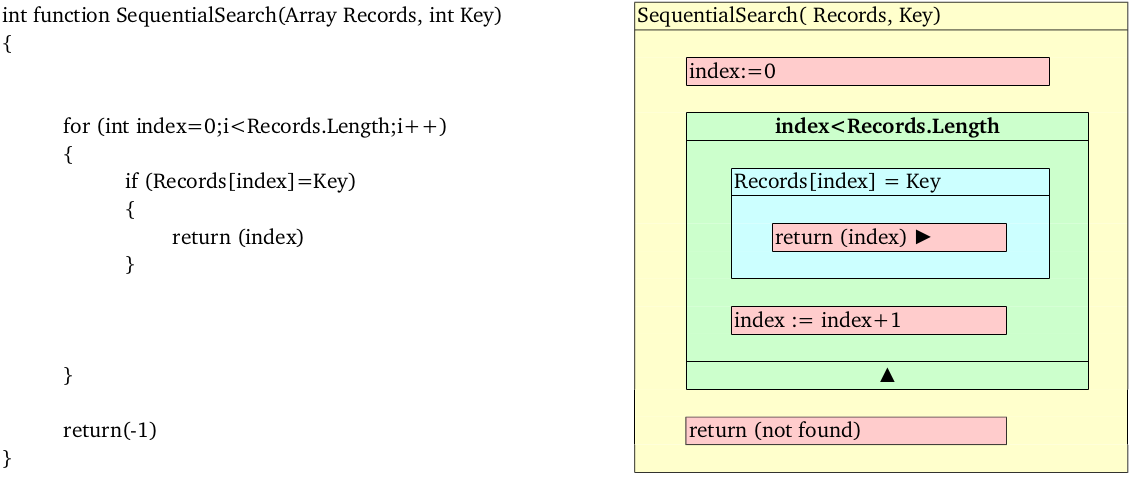
\includegraphics[width=1\textwidth]{chapter2/seqsearchkopenogram.png}
    \caption{Pseudo-code (left) and kopenogram (right) of sequential search algorithm with complexity $O(n)$. The red blocks are commands, i.e. setting the index or returning results. The green block represents the loop with entry condition. The index is incremented and in programming languages this can be done e.g. by \emph{for} cycle statement. The blue block is condition (\emph{if} statement), when fulfilled then the inner blocks are executed, in our case the found index is returned. If no record is found, the loop will end with the last index within \emph{Records} and \emph{not found} sign is returned. }
    \label{fig:search}
\end{figure}

Polynomial time algorithms are defined as the one which time complexity can be bounded by $O(n^k)$ for some constant $k$. Class of problems which are solvable by polynomial algorithm are denoted as \emph{class P} and are recognized as tractable first noted by Cobham or Cook \cite{Cobham1964,Cook1983}. Other algorithms whose time cannot be bounded by any polynomial function are called exponential and are recognized as intractable as published by Garey and Cook \cite{Garey1979,Cook1983}. Because for a relatively small input data the exact solution can be found using the known exponential algorithm with current computation power, however, for bigger input data the time needed to solve the problem is far beyond reasonable amount as seen from Table \ref{table:timecomplexity}.

There were identified a class of problem where it is not known whether a polynomial time algorithm exists, however, if such solution exists, it can be verified in polynomial time -- class \emph{NP-complete}. If some polynomial algorithm will be found in future solving some NP-complete problem, then a derived algorithm will solve other problems within the class of \emph{NP-complete} problems in polynomial time too as denoted by Cook and Karp\cite{Cook1971,Karp1972}. Current best known class of algorithm to solve such problems are based on brute-force search of all possible values and it is open question whether better exists. 

Brute-force search is general solving technique that generates all possible candidates of solution and checks if the problem satisfies the problem statement. All the algorithms to solve brute-force search suffers with exponential time complexity$O(k^n)$\footnote{e.g. depth-first iterative-deepening algorithm for brute-force search was shown to be optimal compared to other standard brute-force search algorithm (depth-first search or breadth-first search)\cite{Korf1985,Pearl1987}.}.

%In the past there were identified several class of problems, for which the current 
%For the class of \emph{NP-complete} problems (non-deterministic polynomial, where if some guess is provided, it can be verified in polynomial time whether it is the solution or not) the current 
%best known algorithm is based on brute-force search of all possible values and better does not exists, or it is open question whether it exists. E.g. For the class of {NP-complete} problems if a polynomial algorithm will be discovered for one problem of this class in future, it was shown that all other NP-complete problems would be solvable by a polynomial algorithm derived from the discovered one\cite{Cook1971,Karp1972}.

%The analysis of complexity of algorithms and problems mentioned above is important for further consequences on computability.
\begin{table}[ht]
\footnotesize
\begin{tabular}{|l|r|r|r|r|}
\hline
\diagbox[height=43pt,width=125pt]{time\\complexity\\function}{input size \\ $n$} & 10          & 20        & 50             & 100            \\ \hline
$n$                                                                           & $00.01$ s     & $00.02$ s   & $00.05$ s        & $00.10$ s        \\ \hline
$n^2$                                                                         & $00.10$ s     & $00.40$ s   & $02.50$ s        & $10.00$ s        \\ \hline
$n^5$                                                                         & $01$m $40.00$ s & $53$ m $20$ s & $14$h $48$m $20$s    & $116$ days       \\ \hline
$2^n$                                                                         & $01.02$ s     & $17$ m $28$ s & $35702$ years    & $4.02\times 10^{19}$ years \\ \hline
$3^n$                                                                         & $59.05$ s     & $40$ days   & $2.28\times 10^{13}$ years & $1.63\times 10^{37}$ years \\ \hline
\end{tabular}
\caption{Computation time of algorithms with different time complexity functions, where one step of algorithm takes 1 millisecond. Examples of algorithm with polynomial time complexity $O(n^k)$ are compared with algorithm with exponential time complexity $O(k^n)$. Note that for the problems with input size of 50 and greater the exponential algorithm runs far beyond the reasonable time compared to the age of universe which is currently estimated to $13.8\times 10^9$  years \cite{PlanckCollaboration2013}.}
\label{table:timecomplexity}
\end{table}

If we presume technological update and the computation speed will increase, the effect of technological speedup is visible in table \ref{table:speedupeffect}. The effect on polynomial algorithm is multiplicative, however for exponential algorithm, the technological speedup will increase the size of computable problem only slightly, this is reason why the problems with only exponential algorithm are denoted as intractable. 
\begin{table}[ht]
\footnotesize
\begin{tabular}{r|c|c|c|c|}
                      & present computer   & 10 times faster               & 100 times faster               & 1000 times faster \\
\hline
\multirow{2}{*}{$n$}  & 3600000        & 36000000         & 360000000        & 3600000000      \\
                      & $1\times$          & $10\times$   & $100\times$  & $1000\times$ \\
\hline
\multirow{2}{*}{$n^2$}                 & 1897 & 6000             & 18973 & 60000            \\
                      & $1\times$          & $3.16\times$ & $10\times$   & $31.6\times$ \\
\hline
\multirow{2}{*}{$n^5$}                 & 20  & 32     & 51    & 81    \\
                      & $1\times$          & $1.59\times$ & $2.51\times$ & $3.98\times$ \\
\hline
\multirow{2}{*}{$2^n$}                 & 21  & 25    & 28    & 31    \\
                      & $N_{2^n}$       & $N_{2^n}+3.32$    & $N_{2^n}+6.64$    & $N_{2^n}+9.97$    \\
\hline
\multirow{2}{*}{$3^n$} & 13  & 15    & 17    & 20    \\
                      & $N_{3^n}$       & $N_{3^n}+2.09$    & $N_{3^n}+4.19$     & $N_{3^n}+6.29$                  \\
                      \hline
\end{tabular}
\caption{ Effect of computation speedup. First value is input size of data computable in one hour, second value is speedup achieved compared to the value in first column. }
\label{table:speedupeffect}
\end{table}

%Note that the age of universe is currently estimated to $13.8\times 10^9  years$ \cite{PlanckCollaboration2013}.
NP-complete problems (currently exponential algorithm can solve them and it was not found better algorithm) are covered in book of M. R. Garey and D. S. Johnson \cite{Garey1979}. The whole complexity theory is covered e.g. in book by Ch.Papadimitriou \cite{Papadimitriou1995} or in a book by M.Sipser \cite{Sipser2012}. 

As that technological speedup will impact mainly the class of problems which are solvable by polynomial algorithm. Other non-exact methods are used to find at least some solution for the problems solvable only by exponential algorithms. These are e.g.: 
\begin{itemize}
\item{The \emph{heuristic methods} tries to eliminate the number of steps of computation by some implicit or explicit knowledge of the specific problem itself E.g. eliminating solution classes that seems not to go to optimal solution. With combination of brute-search the heuristic methods reduce the size of all possible solution candidates to check.}
\item{The \emph{randomization methods} use non-deterministic methods in some level of computation. E.g. Monte-Carlo method is used to compute problems using pseudo-random generated values and after several iterations statistical methods are used to compute expected value and standard deviation. }
\item{\emph{Restriction on input data} - is another form of using the explicit knowledge of the problem instance ad it may reduce all possible values to be checked. }
\item{\emph{Approximation algorithm} - may find not only some good solution, but can quantify how far from the optimal solution the found is good with some degree of probability.}
\end{itemize}

\section{Parallelization}
\label{sec:introparalel}

If a sequence of instructions can be divided into parts which  can be computed independently in parallel by multiple processors, then it is possible to achieve some computation speedup using current computational technology. %Parallel computing can be utilized in several types of application which are further distinguished by the types of location and access to the computation resources. 

A speedup of a computation on P processors can be defined as:
\begin{equation}\label{eq:speedup}
 S(P) = \frac{\text{time on 1 processor}}{\text{time on P processors}}
 \end{equation}

%We can estimate speedup of an computation of a fixed-size problem and then we can ask how can we speedup this problem on P processor. 
In fig. \ref{fig:serialvsparallel} is example of serial and parallel execution computation of the same algorithm.

\begin{figure}[ht]
    \centering
    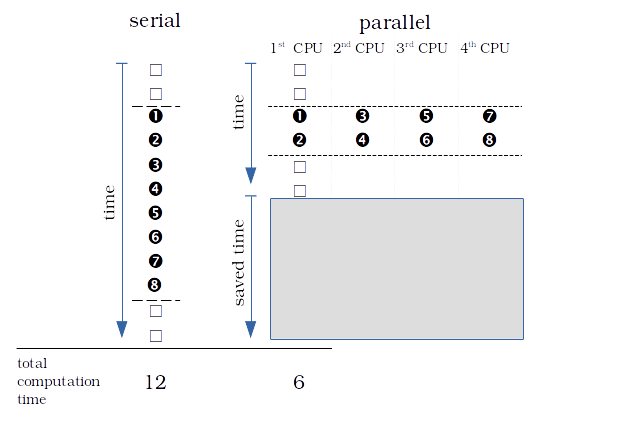
\includegraphics[width=1\textwidth]{serialvsparallel.png}
    \caption{Comparison of serial and parallel execution of instructions. The instructions with numbers can be executed in parallel. In this case the serial computation takes 12 cycles, parallel computation on 4 CPU takes 6 cycles and the speedup is $2$. If we have 8 CPUs, then a computation will be finished in 5 cycles and the speedup will be $2.4$ times.}
    \label{fig:serialvsparallel}
\end{figure}

Assume  $\alpha \in (0,1)$ as a fraction of the computation in one processor which cannot be parallelized, $(1-\alpha)$ is fraction of the computation in one processor which can be parallelized by $P$ processors and $t$ is time needed to compute the process on one processor. Assume that overhead of parallelization is small and can be disregarded. Then speedup can be computed as:
\begin{equation}\label{eq:speedup2}
 S(P) = \frac{t\times\alpha+t\times(1-\alpha)}{t \times \alpha + \frac{t \times (1-\alpha)}{P} } = \frac{1}{\alpha +\frac{1-\alpha}{P}}
 \end{equation}
On unlimited number of processors it can be formulated theoretical upper bound of speedup which depends on $\alpha$ only, denoted as Amdahl's law \cite{Amdahl1967}.:
\begin{equation} \label{eq:amdahl}
S = \lim_{P \to \infty} \frac{1}{\alpha +\frac{1-\alpha}{P}} = \frac{1}{\alpha}
\end{equation}

E.g. when a 33\% of computation cannot be parallelized( $\alpha = 0.33$) then the speedup on 8 processors can be theoretically $S(8) = \frac{1}{0.33+0.7/8} = 2.4$ and theoretical speedup on unlimited number of processors is $S = 1/0.33=3$. See more at fig \ref{fig:amdahl}.
\begin{figure}[ht]
    \centering
    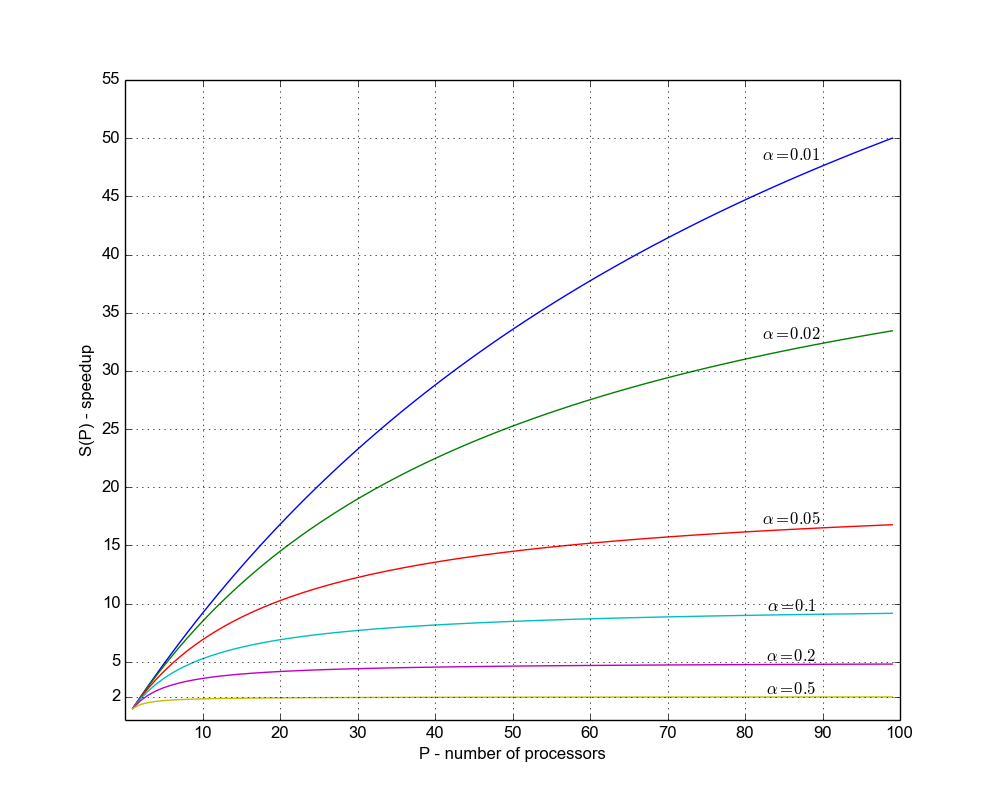
\includegraphics[width=1\textwidth]{chapter2/Amdahl.png}
    \caption{Speedup gained on 1 to 100 processors per Amdahl's law for different $\alpha$ values.}
    \label{fig:amdahl}
\end{figure}

However, $\alpha$ could be sometimes hard to estimate. Additionally, the computing of the fixed size problem on high number of processors can misrepresent the speedup expectation. Therefore, Gustafson reformulated the law and described another approach to measure the fraction of the computation which cannot be parallelized from computing on $P$ processors and estimate the speedup from how long will such computation take on single processor. Assume that overhead of parallelization is small and can be disregarded. The $\beta$ is "scaled fraction" of computation on $P$ processors which cannot be parallelized \cite{Gustafson1988}:
\begin{equation} \label{eq:gustafson}
S(P) = \frac{t \times \beta + t\times(1-\beta)\times P}{t\times\beta+t\times(1-\beta)} = \beta + (1-\beta)\times P 
\end{equation}
This law presumes that the fraction $\beta$ will not change on different number of processors, as seen at fig \ref{fig:gustafson}.
\begin{figure}[ht]
    \centering
    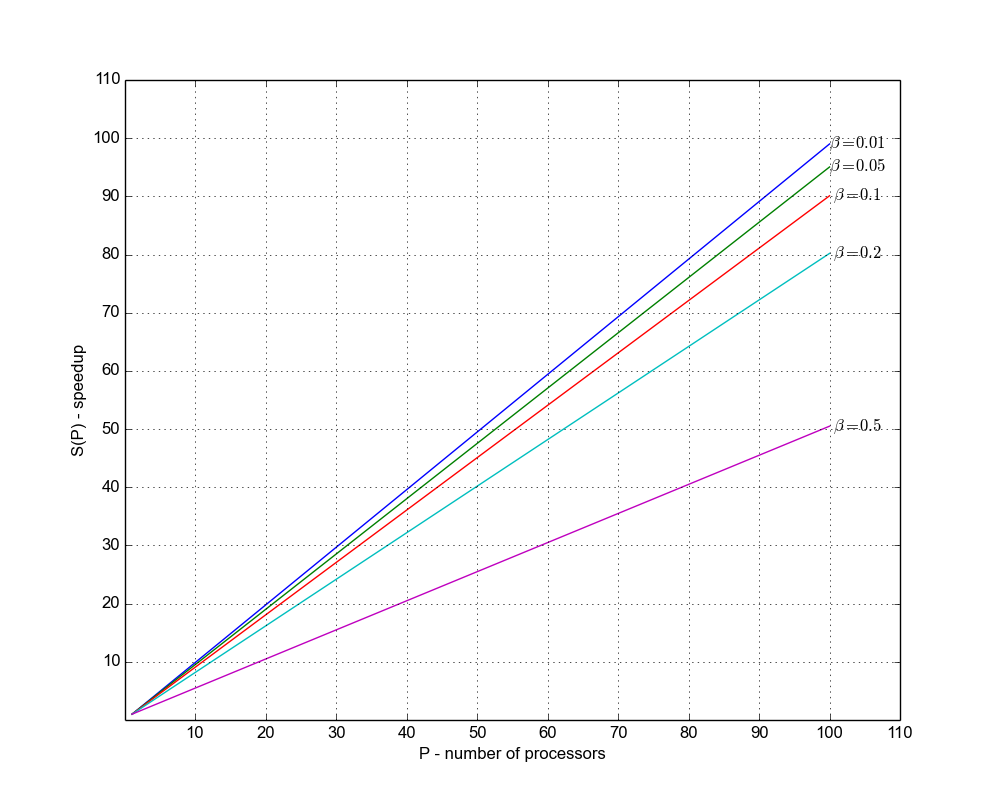
\includegraphics[width=1\textwidth]{chapter2/Gustafson.png}
    \caption{Speedup gained on 1 to 100 processors per Gustafson's law for different $\beta$ values.}
    \label{fig:gustafson}
\end{figure}

Both laws disregard parallelization overhead, however if there is significant one, the speedup of parallelization will be degraded by the overhead. The Amdahl's law (\ref{eq:amdahl}) is argument that the speedup is limited for current sized problem, however, bigger problems can be addressed with higher number of processors and this should be considered rather with regard to Gustafson's law (\ref{eq:gustafson}).

\subsection{Programming model}
\label{sec:parallelprogramming}
There are several levels how the parallelism is realized:
\begin{itemize}
\item{\emph{Instruction level parallelism} -  if the instructions are independent, then they can be executed at the same time by multiple central processing unit(CPU)\nomenclature{CPU}{central processor unit},  e.g. by several cores of the multi-core processor. Programs are usually written as a sequence of instruction and instruction parallelism depends mainly on compiler capabilities to recognize or reorder the instruction to  execute the instruction in parallel. Instruction parallelism started to be systematically utilized in multi-core processor era.}
\item{\emph{Data parallelism} - the same operation is performed on multiple data, usually arrays. The instruction is distributed into multiple processors or processor cores and is executed on elements of data structure in parallel. This is currently characteristic feature of \emph{General purpose graphical processing unit}(GPGPU) computing and programmable API such as CUDA\footnote{\url{https://developer.nvidia.com/cuda-zone} accessed February 2015} and OpenCL\footnote{\url{https://www.khronos.org/opencl/} accessed February 2015}}
\item{\emph{Loop parallelism} - the computation may contain an iteration on some large data structure. Usually such iterative processing is programmed as a loop and if $i^{th}$ iteration is independent on $(i-1)^{th}$ then the iteration can be executed in parallel by different processors.}
\item{\emph{Task parallelism} - the computation contains parts which are independent of each other. Computation of such parts can be scheduled and distributed into multiple processors and can be computed concurrently. E.g. Master/Worker pattern is realized(master sets up a pool of worker processed and a set of tasks which is distributed to them). Fork/Join pattern - main process forks into several threads executing concurrently and waits for their results to join back into a single process which may after some computation again fork.}
\end{itemize}

Looking into the way how the processes interacts, these are the most common forms:
\begin{itemize}
\item{The \emph{threads} are several concurrent execution paths which are independent, but in general share the same memory. It was standardized e.g. as a POSIX threads (Pthreads) and implemented in many platforms.  Further reading about Pthreads can be found in a book by Butenhof \cite{Butenhof1997}. There are other implementation going beyond the POSIX standard is introduced in other languages and programming environment.}
\item{\emph{shared memory}. The \emph{OpenMP}\footnote{\url{http://openmp.org/} accessed February 2015} is a shared memory application interface standardized and implemented in by several compilers for C, C++ and Fortran. It uses also multithreaded model, however, programming is task oriented and more abstract than using threads as described by Chapman et al. \cite{Chapman2008}. }
\item{\emph{message passing}. The \emph{Message Passing Interface}(MPI)\nomenclature{MPI}{Message Passing Interface} is specification for performing task communication by passing messages between tasks. Further reading about MPI can be found in a book of Pacheco \cite{Pacheco1997}.
}
\end{itemize}
More about parallel programming models can be found in survey by Diaz et al. \cite{Diaz2012}.

Some algorithms can be divided easily into independent tasks, which can be computed in parallel. If there is no need to communicate among the parallel tasks, such algorithms are called embarrassingly parallel. E.g. 
\begin{itemize}
\item{Operation on matrices  \cite{Moler1986} are currently used to render 2D and 3D graphics.}
\item{Parameter study, where the same computation is performed using different set of input parameters \cite{Foster1995}.}
\item{Brute-force search algorithm, where subset of possible candidates for solution are generated and checked in parallel.}
\item{Genetic algorithm and other evolutionary algorithms \cite{Cantu-Paz1999}.}
\end{itemize}
In contrast to embarrassingly parallel problems, there exists  inherently sequential algorithms that cannot be significantly speeded up by parallel computing. %The theory about this problems and related algorithm which are denoted as problems/algorithm in class \emph{P-complete} are believed not to get significant speedup using parallel computing, see e.g. book of Greenlaw et al. \cite{Greenlaw1995}. 

Both aspects scalability(speed up gained by parallel computing) and effectivity (time demand based on the size of input data = time complexity) should be considered as highly scalable algorithms can be outperformed by a sequential algorithm solving same problem with better time complexity as noted e.g. by Madden \cite{Madden2012}. 

Further aspects of parallel computing can be found in the earlier book about design and build parallel programs of I.Foster \cite{Foster1995}, book of D.Culler et al  \cite{Culer1998} or book of T.Rauber and G.Räuder \cite{Rauber2013}. 

\subsection{Summary}

To summarize this section; parallel computing can introduce speedup on current computational technology and some computation problems may become feasible.
Additionally, overhead caused by parallelization and fraction of non-parallelizable parts should be considered as it may degrade expected speedup.
In case of exponential algorithm (e.g. for NP-complete problems) the speedup will increase the size of solvable problem only slightly (see table \ref{table:speedupeffect}) and some problems cannot be (or it is believed) significantly speedup by parallel computing. 
In further text a focus will be given mainly to task parallelism and distributed computing. 

\section{Distributed computing technologies}
\label{sec:distributed}

%An important idea is to share computational resources among multiple different users and communities. Several issues needs to be addressed e.g. authentication and authorization using security protocols and database of privileges. Other is scheduling, thus the work of all potential users will not collide in one time and in another time the resources will not be utilized. 
Distributed computing is based on the idea to spread the computation task into set of computers which are connected via computer network.

Main motivation of using distributed computing technologies are (1) sharing, storing and exchanging resources (2) provide and consume computational services (3) access the much higher capacity of storage and computation than available locally (4) connecting the users, developers, people.

To manage distributed computing several challenges are maintained such as synchronization(exchange of messages in computation workflow) to achieve e.g. mutual exclusion(when a task needs exclusive access to some resource) and prevent deadlock(no progress is possible) or resource starvation(when resources - e.g. processor time - is not scheduled for particular task for some reason and task cannot finish computation). Distributed systems offer some sort of fault tolerance (managing fault of a node during computation) or security (encryption of communicating channels and stored data, authentication and authorization to access some resources or data) etc. The topic of distributed computing is covered e.g. in book of Tannenbaum \cite{Tanenbaum2007}. 

An extreme example of distributed computing is Internet where the computers are interconnected via TCP/IP\nomenclature{TCP/IP}{Transmission Control Protocol/Internet Protocol} protocols, the services are provided by servers (e.g. web servers) with some degree of security and fault tolerance. E.g. world wide web is based on HTTP\nomenclature{HTTP}{Hypertext Transfer Protocol} protocol and HTML\nomenclature{HTML}{HyperText Markup Language} language and related technologies, peer to peer services are based on TCP/IP or UDP\nomenclature{UDP}{User Datagram Protocol} and streaming of data.

For scientific purposes, the distributed computing infrastructures evolved into set of clusters, computing centers or individual computing resources owned by different subjects. And an effort is continuously done to join such resources into a federation of computational capacity via high speed network to obtain optionally better virtual capacity in case of need. There were formulated some minimal requirements and defined and implemented standards for network protocols and services that a distributed infrastructure should fulfill and provide. Such infrastructures are currently distinguished as grid-computing or cloud-computing infrastructures and the users of it can get access to much higher virtual capacity than accessible locally. Users also may access remotely specialized devices which are not available within their institution.

%\subsection{Software architecture}
%\label{sec:introintegration}
\subsection{Programming model}
\label{sec:distributedprogramming}

The parallel programming model (section \ref{sec:parallelprogramming}) is used to realize the distributed computing in local computer or server and additionally higher level of task interaction is realized via shared distributed file system or messages passed over computer network. 
Looking into the software layers, distributed computing usually incorporates one or several new layers, some of them are called middleware  delivering services or APIs for application and hides specific implementation across heterogeneous computing platforms(operating system and hardware).

\subsubsection{System Architecture}

As the algorithms and programs needed to solve increasing number of problems and changing requirements, a view on software architecture is needed to construct and order several programs and algorithms into wider robust system aiming to solve broader set of problems.

%The decision about software architecture are made at the begining of a project and are hard to change in implementation is influenced by the experiences that building an application and solution from scratch is too expensive and time consuming. Integrating non-compatible modules might be also time consuming therefore several architecture paradigmas, constraints and patterns are followed to facilitate joining different blocks of software to complex system solving complex problems.

The major software architecture within distributed computing are based on client-server architecture (Example in fig. \ref{fig:architecture}), peer-to-peer architecture or more layered architecture patterns.
\begin{figure}[ht]
    \centering
    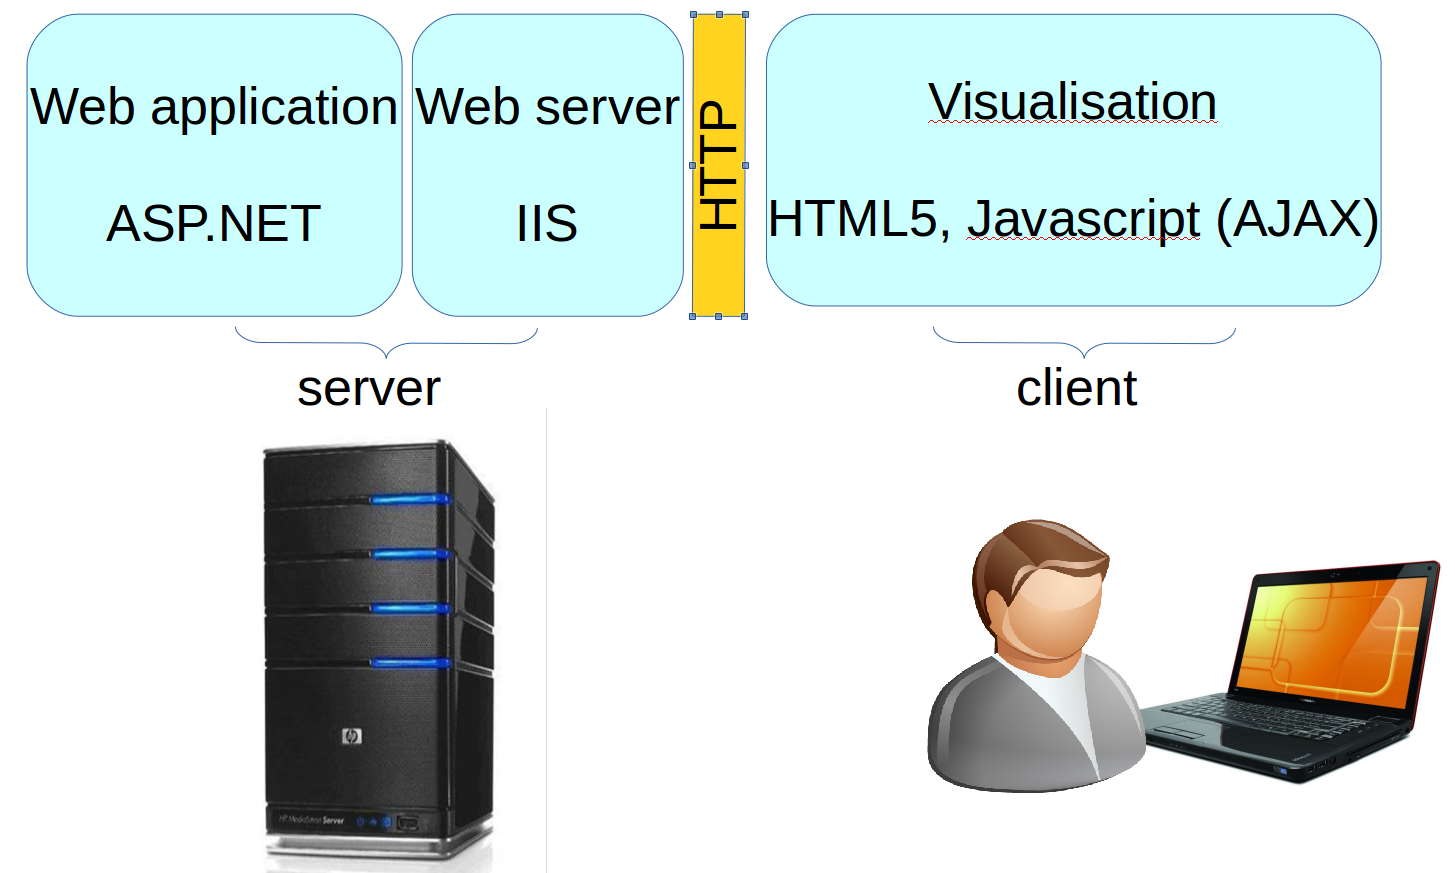
\includegraphics[width=1\textwidth]{chapter2/architektura.png}
    \caption{Example of client-server architecture involving web server which is middleware between web application and server platform. Client visualization in HTML5 web page communicates with server via HTTP protocol.}
    \label{fig:architecture}
\end{figure}

%Client-server architecture consist of two and more layers(tiers) E.g. three tier architecture consists of presentation (client) - logic and data tier (server) and each of the server tiers may reside on different physical resources. Example in fig. \ref{fig:architecture}) shows the web server, which is a middleware delivering some abstract functionality expected such as listening on specific TCP/UDP port, call appropriate functionality or deliver a static document, and such middleware is not implemented by the author of the application who deals only with server specific and client specific part. 
%In recent years several architecture styles are applied.

Service oriented architecture (SOA) is high level programming model based on self contained units of functionality --service -- wrapped with documented interfaces. SOA introduces a new service layer in the client-server architecture which separate service interface from its implementation. SOA principles and paradigms are described e.g. in book of T. Erl. \cite{Erl2008}. 

Another approach represents objects and data of the system as resources with standard set of operations, create, read, update, delete (CRUD)\nomenclature{CRUD}{Create Read Update Delete}. Representation State Transfer (REST)\nomenclature{REST}{Representation State Transfer} specifies several architectural constraints that help scalability, performance and presents functionality via fixed number of operation and uniform resource location proposed by Fielding \cite{fielding2000chapter}. The REST style constraints towards the application is statelessness, resource orientated with uniform interface (CRUD) and hypermedia driven which should facilitate and optimize processing of resources via current web based technologies, mainly HTTP protocol. 

While SOA focus on application design and easily turning the application objects into distributed services, REST is rather set of constraints to the architecture to handle the issues of distribution within web, as noted e.g. by Vinoski \cite{Vinoski2007}.

Software architecture of the enterprise application, distributed systems and some repeating patterns are cataloged e.g. in a book by Fowler et. al\cite{Fowler2003} or Nilsson \cite{Nilsson2006}. Integration patterns are discussed with focus on the ways of connecting heterogeneous parts of the system by Hohpe et al.\cite{Hohpe2002}.
\subsubsection{Types of computing infrastructure}
When we focus on the architecture of the middleware and philosophy of building a computing infrastructure, these main types of distributed infrastructures are distinguished for scientific computing and are relevant to the rest of this work:
\begin{enumerate}
\item{\emph{Service grid-computing} is based on the idea that a computing resources (servers, clusters, special hardware) is owned by some organization but may be maintained by some collective organization with an effort to provide a collection of services in best effort approach.}
\item{\emph{Desktop grid-computing} is based on the idea to connect generic desktop computers and provide the idle computation time e.g. as a screen saver or background process to the projects.}
\item{\emph{Cloud-computing} provides architecture to services, platform or whole infrastructure in a way that access to them is provided as a service with an impression of sole use it by user or process.
}
\end{enumerate}

\subsection{Research and education network}
The fundamental part of any Grid is the computer network connecting resources that are distributed in different geographical location, generally Internet. 

The national grid initiative in Czech Republic 
-METACENTRUM\footnote{\url{http://www.metacentrum.cz} department of CESNET as national grid infrastructure} is interconnected via high-speed network CESNET 2 utilizing the technology of transferring data over optical cables using Dense wavelength division multiplexing (DWDM)\nomenclature{DWDM}{Dense wavelength division multiplexing} \cite{novak2007deployment} ad seen in fig. \ref{fig:cesnet}.

\begin{figure}[ht]
    \centering
    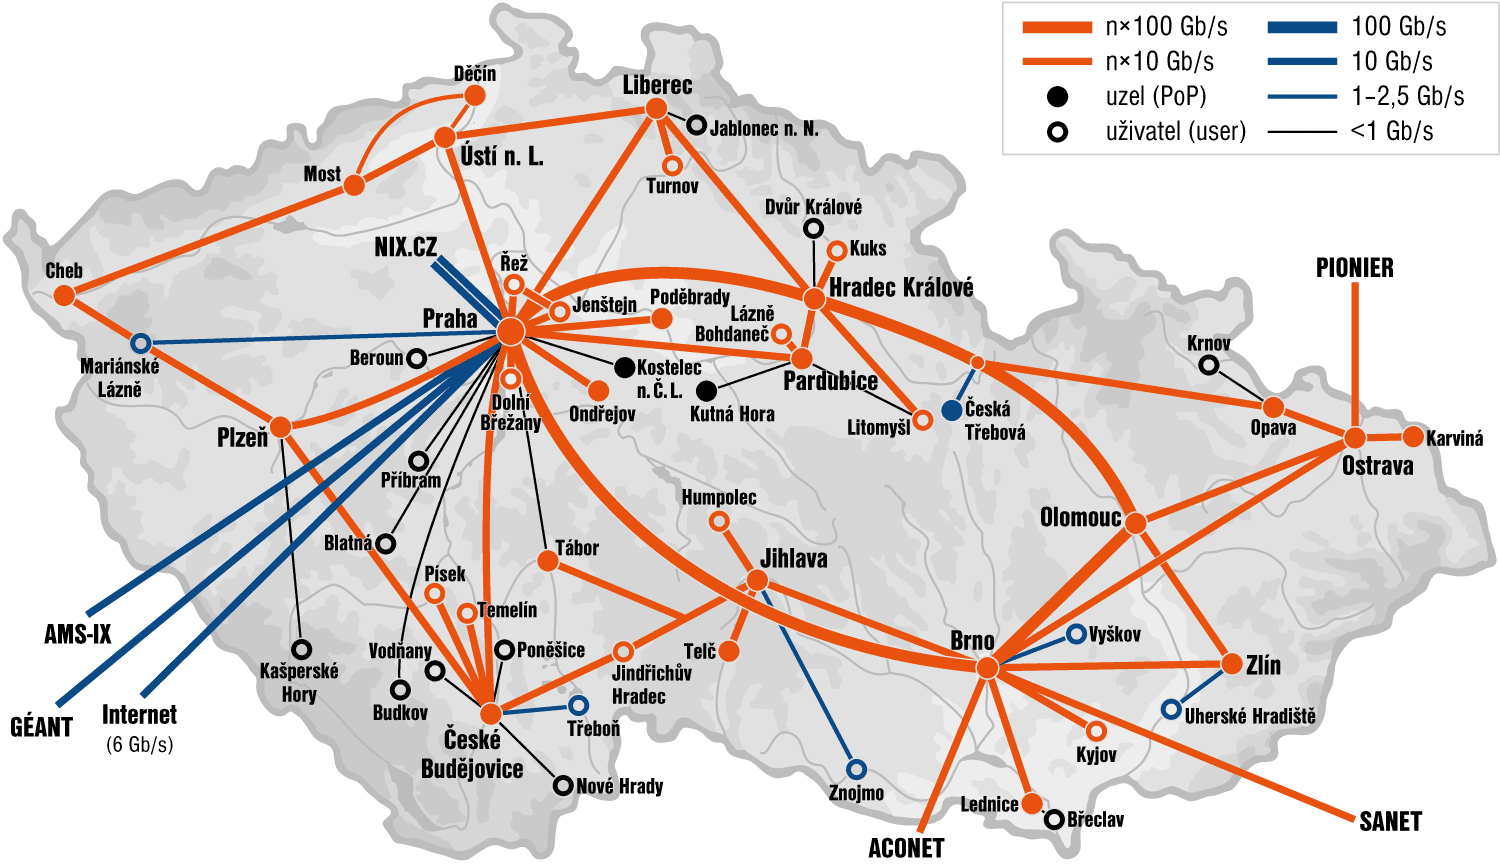
\includegraphics[width=1\textwidth]{chapter2/cesnet2-topo1.png}
    \caption{CESNET2 network topology as from december 2014 is maintained by association of universities and academy of science CESNET. Interconnects mainly departments of universities and academy of sciences via rented physical network. It provides connection to general Internet via the czech NIX.cz (Neutral Internet eXchange), AMS-IX (Amsterdam Internet eXchange) and other channels to European research and education network GÉANT. Sources: \url{http://www.cesnet.cz}}
    \label{fig:cesnet}
\end{figure}

\subsection{Service grid-computing}
\label{sec:servicegrid}

The Service-grid computing is based on a basic set of services implemented by a middleware to provide uniform interface for job scheduling and execution within the computing infrastructure. The term \emph{Grid} is used to emphasize the analogy with the electric power grid providing access to electricity \cite{foster2004}. Foster et al.\cite{foster2001,foster2004} and Chervenak et al. \cite{Chervenak2000} describe "data" and "computational" grid as shared hardware and software resources that provide reliable, consistent, pervasive and cheap access to high performance computational capacities and  effective and reliable execution of requests over data, which needs sensitive controlling of terabyte storage, data transfers to gigabits per seconds over global computer networks and scheduling such data transfer with respect to computational needs. The services provided by grid are either tools or web services following  \emph{Service Oriented Architecture}(SOA)\nomenclature{SOA}{Service Oriented Architecture} for grid computing -- Open Grid Service Architecture (OGSA)\nomenclature{OGSA}{Open Grid Service Architecture} \cite{Foster2003}. The security model and access to the grid infrastructure is proposed and implemented mainly by a mutual authentication between users and resources via public key infrastructure using X.509 certificate \cite{Foster1998}.
The administration and maintenance of such networked infrastructures are not trivial tasks and they are performed by experts of institutional computing centers or national laboratories and interconnected sites are managed and coordinated at national level or at international level. Such national organizations cooperate with similar national grid infrastructures in other countries. An umbrella organization in Europe --European Grid Infrastructure (EGI)\nomenclature{EGI}{European Grid Infrastructure}\footnote{\url{http://www.egi.eu}} -- was established during 2010 and supports integration and coordination activities of national grid initiatives (NGI)\nomenclature{NGI}{National Grid Initiative} across national boundaries with respect to the scientific collaboration which goes also across national boundaries. 

\begin{figure}[htb]
    \centering
    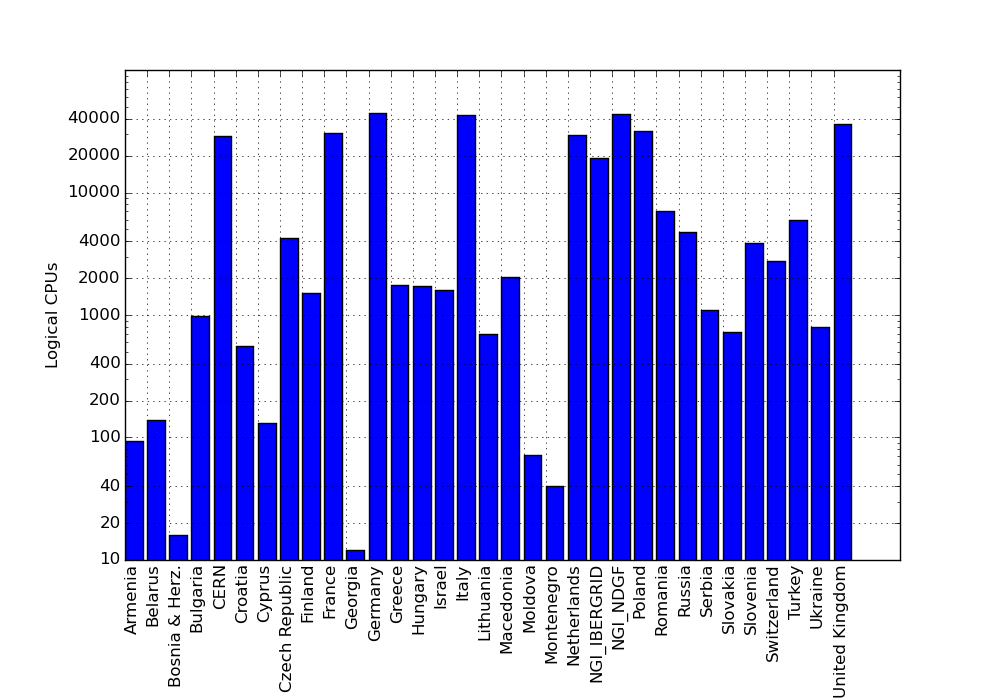
\includegraphics[width=1\textwidth]{chapter2/egicpus.png}
    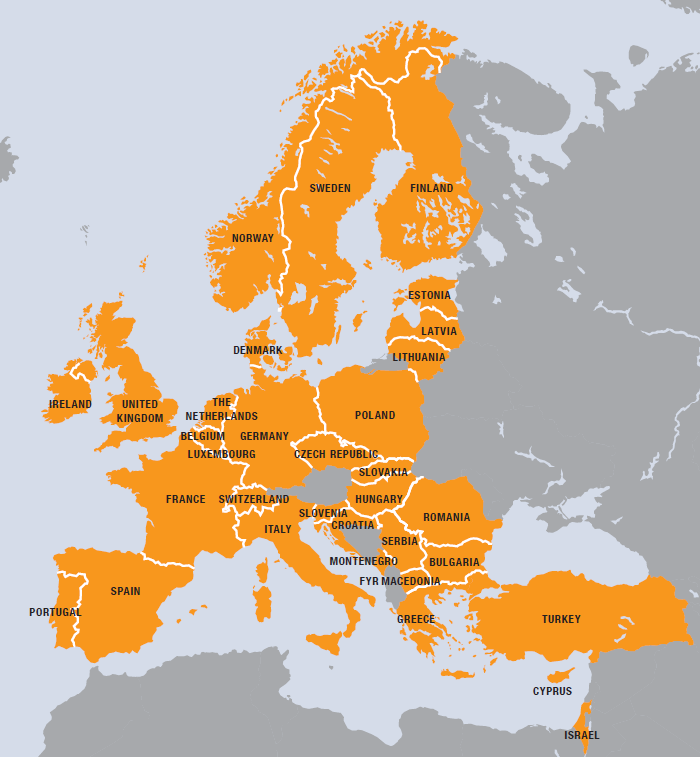
\includegraphics[width=0.6\textwidth]{chapter2/egi.png}
    \caption{Countries involved in EGI and number of CPUs within EGI infrastructure in 2012, the total logical CPU capacity at the end of 2012 was 349,720 cores( in graph per countries). CPU capacity was 433,957 cores in March 2014. Sources: EGI Compendium 2013, EGI statistics at \url{http://www.egi.eu}.%\bibentry{EGICompendium2013} \bibentry{egi2014}.
    }
    \label{fig:egi}
\end{figure}

The growth of several production grid infrastructure for science was accelerated in last decade mainly by the needs of experiments of high energy physics to process large number of observed data in a reasonable time \cite{Bird2009}. The Worldwide Large Hadron Collider Computing Grid (WLCG)\nomenclature{WLCG}{Worldwide Large Hadron Collider Computing Grid} has been designed to store and process almost 30 PetaBytes of data per year in the period of 2009-2013  \cite{Adamova2014} and is one of the largest grid deployed in the grid infrastructure. As the hardware infrastructure is built with a philosophy of federated access to resources owning by research institution, universities etc, other scientists from different scientific disciplines can become users of this powerful infrastructure too. The development of virtualization, the infrastructure may employ larger set of application and services and may become attractive for smaller scientific collaboration.

Several grid infrastructures were established based on different grid-middlewares.
Condor is one of the earliest effort to provide access to underutilized computers while preserving rights of the owners \cite{Litzkow1990}. glite \cite{Laure2006}\footnote{\url{http://glite.cern.ch} accessed February 2015}, ARC\footnote{\url{http://www.nordugrid.org/arc/} accessed February 2015} and Globus \cite{Foster1997}\footnote{\url{http://toolkit.globus.org/toolkit/} accessed February 2015} are major grid-middleware operational in EGI.

Currently there is an effort to maintain interoperability to connect different application with different resources from the different grid infrastructures. Riedel et al. reports on such effort to involve technology providers as well as deployment teams to participate on open standards for security, data management etc. \cite{Riedel2009}.

\subsection{Desktop grid-computing}
\label{sec:desktopgrid}
Joining desktop computers from an individual user to form a voluntary or desktop-grid was popularized by a project trying to identify uncommon signals from space to search extraterrestrial intelligence (SETI@Home)\footnote{\url{http://setiathome.ssl.berkeley.edu/}}. It's based on the idea that a volunteer will download a small client program, which executes in background or instead of a screen saver; it downloads some amount of raw data from a server on Internet to analyze and sends back the result to the server. In contrast to service grids, the authorization of users can't be so strong for volunteer individuals and some other policies, e.g. redundancy, is implemented to eliminate bad or cheating results \cite{Anderson2002}. After the success of the SETI@Home there were built general-purpose frameworks to facilitate development of projects that will use similar philosophy of computing on desktop computers connected via Internet such as BOINC\nomenclature{BOINC}{Berkeley Open Infrastructure for Network Computing} \cite{Anderson2004}, SZTAKI extension to BOINC \cite{Balaton2007,Kacsuk2009}, XtremWeb \cite{Fedak2001} and others. Currently there exists lot of similar projects gaining computer power as the SETI@Home project. E.g. the LHC@Home and it's successor LHC@Home 2 projects were established and used to execute some selected tasks of the Large Hadron Collider (LHC)\nomenclature{LHC}{Large Hadron Collider} project on the desktop grid infrastructure \cite{Herr2006,Hoimyr2012}.

The average performance of BOINC projects is 8.073 PetaFLOPS  with active 294~764 volunteers computing on 502~238 computers (March 18$^{th}$ 2015). E.g. SETI@Home 24 hour performance is 1.95 PetaFLOPS. Although desktop grids and service grids are two different approaches to gather computing power from large number of computing resources, there is an effort to interoperate and e.g. share capacity for a project, e.g. EdgE project published by Kacsuk et al.\cite{Kacsuk2008}  and Urbah et al. \cite{Urbah2009}.

\subsection{Virtualization}
\label{sec:introvirtual}
Virtualization technology separates the physical hardware layer from the software environment emulating a new virtual hardware layer. Hypervisor or virtual machine manager manages guest virtual machines, translates I/O\nomenclature{I/O}{Input Output} operations between virtual device and physical device, translates instructions from virtual CPU to physical CPU. This introduces some overhead and performance degradation of virtual system compared to physical. However, recent virtualization technology introduced several techniques which reduces overhead and eliminate specific hardware features and instructions which are hard to virtualize as reported by Barham et al. and Youseff et al. \cite{Barham2003,Youseff2006}.
Thanks to them, a virtual environment fine tuned for an application can be executed on almost any hardware and platform and virtualization becomes part of the solution to execute jobs of desktop-grid or service-grid computation on different physical platforms \cite{ruda2009virtual}.
Currently there exists several commercial, free or even opensource virtualization implementation which are provided by different vendors and it's hypervisor - VMWare\footnote{\url{http://www.vmware.com/} accessed March 2015}, XEN\footnote{\url{http://www.xenproject.org/} accessed March 2015}, KVM\footnote{\url{http://www.linux-kvm.org/} accessed March 2015}, VirtualBox\footnote{\url{https://www.virtualbox.org/} accesse March 2015} etc. 


\subsection{Cloud computing}

In contrast to grid-computing where user scheduled jobs accessing shared environment and might be influenced by other users or by the environment, the cloud-computing provides access to a virtual software, platform or whole infrastructure so the user or process has impression of sole use. Virtualization techniques enabled expansion of cloud-computing mainly on infrastructure which was built for another purpose and can be rented in times when the primary infrastructure is not fully utilized \cite{Foster2008}. 

Cloud-computing can be characterized as a model for enabling ubiquitous, convenient, on-demand network access to a shared pool of configurable computing resources (e.g., networks, servers, storage, applications, and services) that can be rapidly provisioned and released with minimal management effort or service provider interaction \cite{Mell2011}.  

Cloud computing makes computational power and storage as utility or commodity that can be rented. It evolves in commercial area to facilitate scaling up the business needs with computational demand with current commercial clouds such as Amazon EC2\footnote{\url{http://aws.amazon.com/ec2/} accessed February 2015}, Microsoft Windows Azure \footnote{\url{http://azure.microsoft.com/} accessed February 2015}, Google cloud\footnote{\url{https://cloud.google.com/} accessed February 2015} and others.

Cloud computing in research infrastructures were recently deployed next to the already existing grid-infrastructures and utilizes the same hardware resources. Some methods to integrate grid-computing and cloud-computing were proposed by Anjum et al. \cite{Anjum2012}. Access is provided to the same users of grid-infrastructure and currently most used platforms are Open\-Nebula  \cite{Milojicic2011} and OpenStack \cite{Kumar2014}.

An interoperability among cloud providers and standardization on cloud-computing, virtualization and related technologies is important as it would keep users from being locked into a specific cloud provider\cite{Ortiz2011}.

\subsection{Application model}

The application computed within grid or cloud can be characterized by the quantity of tasks being performed, the size of input data and of the communication needs to be done between concurrent tasks. 
Grid-computing infrastructures were primarily utilized for computation, which tasks take long time, were relatively loose coupled and resources were used over long period. Performance/capacity is usually mentioned  in operations/CPUs per month or year and for such computation the term High throughput computing (HTC)\nomenclature{HTC}{High throughput computing} is used.

While HTC takes long time, the High Performance Computing (HPC)\nomenclature{HPC}{High Performance Computing} is usually characterized by computing the problems which have small number of tasks and are relatively tightly coupled and can be executed in highly parallel environment. Performance is measured usually in operations per second  \cite{Hager2010,Levesque2010}. The grid infrastructure can involve HPC servers or clusters, thus a job or tasks that requires such HPC hardware are scheduled and executed there.

Many Task Computing(MTC)\nomenclature{MTC}{Many Task Computing} aims to bridge HTC and HPC, while the computation usually takes shorter time, the data exchange is in MB rather in GB, performance is measured in tasks per seconds rather than jobs per months or years and involves computing relatively much more heterogeneous problems which are not "happily" parallel. However, middleware for HPC or HTC which are present in grid-computing infrastructures may introduce some shortcomings, therefore a prototype task execution framework suitable for MTC was proposed and implemented by Raicu et al.\cite{Raicu2008, Raicu2009,Raicu2010}.
The MTC seems suitable to be performed on cloud-computing technologies, which introduces some benefits over classical grids, however such clouds should be oriented for HPC systems and generic public cloud may introduce low performance than expected \cite{Iosup2010}.

\subsection{Workflows and Gateways}
\label{sec:introworkflow}
A workflow is an abstract description of the process of computation and data manipulation specified by an expert to express what should be done within the distributed system. It automates the process of computation by composing data manipulation steps and tasks and solving failure events.

The workflow can be encoded in any programming or scripting language, however some higher level languages evolved. In business domain a Business Process Execution Language (BPEL) is an OASIS standard and becomes one of the most used language for describing workflow of orchestration of web services and transaction steps \cite{Pasley2005}. In scientific domain different workflow systems are operational including BPEL with different capabilities. Taxonomies of some existing workflow systems were published by Yu, Zhao et al. \cite{Yu2005a,Zhao2008,Curcin2008}. Workflows in cloud computing are covered by web technologies programming languages (Javascript) \cite{Foster2008}.

The workflow system which implements the concrete workflow language is usually tightly coupled with the specific grid-computing or cloud-computing infrastructure. 

To connect different grid-infrastructures a mutual workflow management system is used to integrate them as proposed by Kacsuk et al. \cite{Kacsuk2008a,Kacsuk2011} or an interoperability is solved by separating abstract workflow representation and concrete implementation showed on selected existing workflow systems introduced by Planensteiner et al. \cite{Plankensteiner2013}.

Scientific gateway incorporates higher level services for specific scientific community e.g. as a web portal or desktop application to control the process of computation via a workflow\cite{Wilkins-Diehr2007}. For building the scientific gateways several frameworks were developed e.g. Apache Airavata \cite{Pierce2014,Memon2014} or WS-PGRADE/gUSE\cite{Kacsuk2012}. And the concrete instances are available for broader area of scientific community. 


%\section{Informatics in Medicine and Biology}
%\label{sec:biology}


\chapter{Methods}
\label{sec:methods}

The general issue of utilizing grid computing or cloud computing infrastructure is to select appropriate method to integrate domain specific computation into the grid or cloud infrastructure of a concrete provider. 

A lot of tools are already available within current grid infrastructure including open-source or licensed software for computation. A list of available application is usually given by the local scientific provider\footnote{applications available in CESNET METACENTRUM \url{https://wiki.metacentrum.cz/wiki/Kategorie:Applications} accessed February 2015} or application database are available in broader environment e.g. in EGI.eu application database\footnote{\url{https://appdb.egi.eu/} accessed February 2015}.
Additionally,  workflow systems and scientific gateways mentioned in section \ref{sec:introworkflow} tries to hide the complexity of grid-computing or cloud-computing infrastructure and may be used to integrate specific domain too.
The programming model of parallel computing and/or distributed  computing (in section \ref{sec:parallelprogramming} and  \ref{sec:distributedprogramming}) needs to be followed when designing new application utilizing benefits of grid-computing and/or cloud computing.

The general approach to port application to grid infrastructure is to automatize what can be automatized, i.e. make scripts, configure system, prepare some user interface, integrate with existing applications, utilize protocol compatibility etc. An effort to obtain first results is high, however if the prepared templates, script or application is reused for further computational request an effort is much lower.  

\section{Sharing medical information}
\label{sec:imaging}
%\label{sec:medicalapp}
%Acquiring, storing and processing digital medical images 
%This chapter introduces acquiring, storing and sharing digital medical images and related metadata within hospital or healthcare provider and among them and research institution.

%are covered in section \ref{sec:introimages}. Overview of analysis of speech and voice and it's relation to voice science is in section \ref{sec:introvoice}. Overview of models and simulation of human physiology and it's relation to systems biology is briefly covered in section \ref{sec:intromodels}.


%The computing in biomedicine can be divided into research and clinical application. %Translational science aims to "translate" findings from research to better health care including diagnostic tools, procedures, drugs, etc.

%In case of research use-cases, processing medical information helps to make more precise current theories or support formulating new one. In case of clinical use cases, processing medical information helps to analyse and interpret the information, predicting future trends and support decision on some intervention.

%\footnote{Motivation of using distributed computing technologies is to share physical data, among multiple organizations, where there is no need or other barriers to store all data centrally, e.g. for legal or capacity limitation. A lot of medical information within biomedical research came from real patient and such information are protected by some regulation and processing of them is regulated and controlled by the country laws or international agreements. Thus there must be considered ethical as well as legal issues how to deal with such information. Sharing and processing of medical images are covered in section \ref{sec:introimages}. Providing access to services with high values is another motivation of using distributed computing technologies. E.g. basic and advanced analysis of biological signals, especially of voice is described in section \ref{sec:introvoice}.}


Use cases related to digital medical images involves the image acquisition, preprocessing, storing and searching.
Clinicians use patient image mainly for visualization and diagnostic purposes. Computer assisted methods facilitate the diagnostic process and involves image enhancement (to reduce image noise and increases the contrast), image segmentation (to separate different types of structures from background and from each other), quantification methods (to determines the structure shape, size, volume), registration methods (to process and join multiple different images into one).
Comprehensive concepts and digital techniques in medical imaging are presented e.g. in book edited by I.N.Bankman\cite{Bankman2000}.

Acquisition of the medical image is covered with different modalities (different types of equipment and sensors) by radiologists or other specialists. DICOM\footnote{DICOM: \url{http://dicom.nema.org/} accessed January 2015}\nomenclature{DICOM}{Digital Imaging and Communication Protocol} format and protocol becomes actually an industrial standard to exchange medical images electronically and picture archiving communication systems (PACS) holding the acquired DICOM images with metadata and description noted by experts are currently part of information systems in hospitals. See the typical workflow of medical image in hospital in fig. \ref{fig:pacs}.

\begin{figure}[ht]
    \centering
    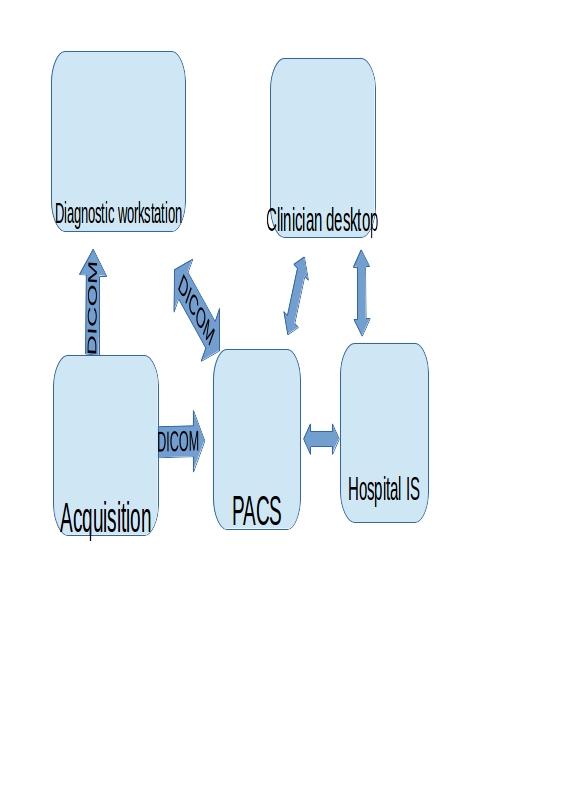
\includegraphics[width=0.8\textwidth, height=8cm]{chapter4/pacs.png}
    \caption{Typical workflow of medical image in hospital. Data acquisition is made by modalities (magnetic resonance, ultrasonography, X-ray radiography, etc.) and using DICOM format and protocol it can be directly transferred and visualized by diagnostic workstation. With metadata filled by an expert physician the image is stored in PACS. Other desktops within hospital can retrieve the image and review the report. The hospital information system may be involved in other workflows and communicate with other formats and standards (HL7,...)
    }
    \label{fig:pacs}
\end{figure}

As the data processed in hospital information systems contains sensitive information of real patients, these are protected and processing and storing is regulated by the national or international laws or agreements.
Development of telecommunication and network technologies a enabled telemedicine -- providing healthcare over remote distance. It requires to share and exchange  sensitive data of real patient among different healthcare providers and such data may be very valuable for further research. Security and encryption should be addressed and DICOM standard itself doesn't solve security issues appropriately, thus encryption during transferring the data over computer network must be ensured by other techniques.

In the Czech Republic, there exists several projects in production interconnecting different hospitals, clinics and other healthcare organization to exchange medical images. Project ePACS allows interconnecting each participant's PACS system via dedicated Virtual Private Network VPN\nomenclature{VPN}{Virtual Private Network} channel to the central node and exchange of medical images are realized by routing the data flow from one VPN channel to the other\footnote{ePACS:\url{http://www.epacs.cz}, accessed January 2015}. Another approach is used in the project MEDIMED held by Masaryk University in Brno. Instead of dedicated VPN channel, they use Secure Sockets Layer (SSL)\nomenclature{SSL}{Secure Sockets Layer} encryption over standard TCP/IP communication and regional hospitals and healthcare providers are interconnected via the MEDIMED servers as presented by Slavicek et al. \cite{Slavicek2010}.% \cite{Javornik2011,Zatloukal2012}.
In other countries, there were tested cross-border teleradiology in projects Baltic e-health, R-Bay and others published by Ross et al. \cite{Ross2010} and Saliba et al. \cite{Saliba2012}.
These projects are focused on sharing the medical images and other knowledge and information.

Access to the wide range of medical images is needed for research of new processing and diagnostic methods, rare diseases, developing new detection algorithm etc.  DICOM records "de-identified" (identification of patient records are deleted, only date of the bird and other data are kept) or anonymized (additional information are manipulated to prevent disclosure) for research purposes to protect sensitive personal data, but keep important information for research purposes. The Globus MEDICUS project published by Erberich et al.\cite{Erberich2006,Erberich2007} is based on Globus Toolkit middleware to federate clinical and research application via a grid-computing infrastructure. Currently the project is hibernated since 2008 and no further development was published\footnote{\url{https://dev.globus.org/wiki/Incubator/MEDICUS} accessed February 2015}. Similar effort was done with a project Medical Data Manager which uses gLite grid middleware published by Duque, Montagnat et al.\cite{Duque,Montagnat2007} \footnote{\url{http://modalis.i3s.unice.fr/softwares/mdm/start} accessed February 2015} or MediGRID project published by Krefting et al.\cite{Krefting2009, Krefting2010}. Additionally, processing of images within selected use-cases supported by the grid-computing infrastructure is introduced\cite{Krefting2010}. Health-e-child project aimed to interconnect research institution and hospitals in United Kingdom, France and Italy for the purpose of grid-based healthcare platform for pediatric health-care \cite{Skaburskas2008}. Neurist project developed architecture and connects clinicians and researchers to improve research and treating of cerebral aneurysm to provide tools to analyze and interpret patient data and researcher can have access to set of aneurysm data, published by Benkner et al.\cite{Benkner2010}.
SEAGRIN research project aimed to  share knowledge mainly for educational purposes in semi-formally described semantics and such proposal and implementation was published by Kuba et al.\cite{Kuba2006}. 

Storing the sensitive medical information even de-identified or anonymised is usually restricted and this lead to an idea to store such information within trusted institution e.g. hospital and move and facilitate deployment of the grid services storing medical data to that institution. E.g. pre-installed virtual machines can contain grid-services and deployed in as a sealed grid as proposed by Kuba et al. \cite{Kuba2007a}.


%When we look to the architecture of the systems of sharing medical images the problematic part within the point-to-multipoint architecture is the central part of the systems already in production e.g. in Czech Republic (MEDIMED, ePACS). This may become single point of failure and bottleneck.

To summarize this section, digital medical image acquisition, store, exchange and processing became common in the past years and is currently using distributed computing techniques. There are several efforts to implement medical data management within grid or cloud infrastructure for research purposes and integrate them with the production infrastructures. Security is solved by authentication, authorization mechanism as well as by encrypting the data and/or de-identification or anonymization but keeping minimal information required for research purpose. A related question is  how easily the previously mentioned grid-based technologies can be integrated with current systems in hospitals or institutions. The following section describes selected methods used to integrate a pilot deployment of Globus MEDICUS with current regional system for exchanging medical images - MEDIMED.

\subsection{Methods to share medical images in grid}
\label{sec:methodsimages}

Globus toolkit belongs to the group of most used grid middleware (see section~\ref{sec:servicegrid}). The core services included in Globus Toolkit are GridFTP -- grid extension to file transfer protocol(FTP)\nomenclature{FTP}{File Transfer Protocol} implements strategies such as \emph{stripping data} into multiple pieces, \emph{parallel transfer of data} utilizing stripped data parts to be transfered via different channels, \emph{partial file transfer} some application may not need to access the whole file, but a smaller portion of it etc. as described by Foster et al. and Allcock et al. \cite{Foster2006, Allcock2005}. Other core services are Replica Location Service aiming to localize data, Globus Resource Allocation Management (GRAM) provides web service and proxies to the lower level job schedulers implementation \cite{Foster2006}.

Next to core services, the domain specific services might be implemented for the purpose of application using the open grid service architecture (OGSA). Globus MEDICUS \cite{Erberich2006,Erberich2007} contains a DICOM Grid Interface Service (DGIS) and integrates the open source PixelMed\texttrademark ~Java DICOM Toolkit\footnote{\url{http://www.pixelmed.com/} accessed February 2015} into a web service communicating via DICOM protocol and on the other side it forwards the queries to underlying services within Globus toolkit. 

DGIS behaves as a gateway to a grid infrastructure. Because communication via DICOM protocol is not secured, the DGIS is recommended to be installed on the location of the PACS system or DICOM ready modality or software.
When a DICOM study is uploaded into DGIS, it is anonymized and stored and a record is made into another services Meta Catalog service which resides in the same domain or anywhere in grid accessible via Globus Toolkit.
Such anonymized database of DICOM records can be used to query via DGIS interface and to e.g. integrate with web based application showing records for research purposes, authentication and authorization can be done in this level. 
To integrate this system with existing system for sharing the medical images (e.g. the MEDIMED project\cite{Slavicek2010}) the special client software "RediMed console" needs to be installed next to the DGIS and configured it as a local PACS system whose records might be exchanged to other MEDIMED participants. 
The results of this particular deployment and integration is in section \ref{sec:resultsimages}.
%The software for processing medical images can retrieve them from DGIS via DICOM protocol. 

%To present DICOM studies The integration strategy based on shared database or files can be used to present the DICOM studies via web portal. Additionally the web portal might generate specific DICOM queries to DGIS.


%The following section will cover methods related to the integration effort.

%The section~\ref{sec:introintegration} describes several general software architectural styles and integration patterns used in further in this work. 
%The section~\ref{sec:methodsimages} describes specific methods used in the area of processing  medical images within grid infrastructure to verify the integration effort between research and hospitals systems. The section~\ref{sec:methodsvoice} describes a method to deploy existing application as a service to the distributed infrastructure.The section~\ref{sec:methodsmodels} focus on modelling methodology in order to build and maintain complex models of human physiology as the complex models seems to mainly benefit from parallel computation. And the subsection~\ref{sec:methodsmodelsestimate} follows up on the modeling methodology to describe the system for estimating model parameters. 

%as a program to start within remote session and , the interactive application allows select type of voice which will be analysed. After recording is finished, the whole recording is analyzed with FFT to obtain full spectral analysis. 

%\section{Integrating heterogenous systems}
%\label{sec:introintegration}
%
%Integrating heterogenous system into a well designed enterprise application has some issues which needs to be addressed.
%
%One of the first decision which may be hard to change in future is platform. Platform might be determined by third party platform-specific product incorporated in a workflow which cannot be changed. There exists software platforms that may run on different operating systems. E.g. Java platform is based on the idea that a program is compiled into bytecode which is then interpretted by just-in time compilers on target platform. Similar approach applies to Common Language Infrastructure (CLI) known by it's implementation .NET Framework on Microsoft Windows operating system or MONO which is implemented on Linux platforms.
%Another approach to address the issue of a platform is virtualization as mentioned already in section \ref{sec:introvirtual}.
%
%
%%\subsection{File exchange}
%Is based on the fact, that one process produces a file which is consumed by another process. This is popular in batch processing systems which needs no or only limited interactivity with user. The grid workflow management systems 
%\subsection{Message Oriented Integration}
%The processes that run concurently synchronize and exchange messages via some dedicated channel. E.g. platform depended
%
%\subsection{Service Oriented Architecture}
%\label{sec:methodssoa}
%Service oriented architecture (SOA) decouples a service contract with intention to be platform independent from it's platform-dependent implementation\cite{Erl2008}. The loosely coupled modules conforming the SOA style are realized as web service which contracts are described in Web Service Definition Language (WSDL) which defines the service interface in term of endpoint location (URL), sset of operation, binding of operation to endpoint, the format of input and output messages and binding of the messages to the operations. These are usually based on some XML dialect. Even the WSDL can be written by hand, it can be generated by a service stack framework for the concrete service implementation. 
%Next to the service implementation there are abstraction like registry and repository holding metadata of the service, so it can be dynamically discovered.
%
%\subsection{RESTful web services}
%\label{sec:methodsrest}
%The Representational State Transfer (REST) architectural style proposed by R. Fielding\cite{fielding2000chapter} is used for representing functionality as a limited  for solving demand issues of the selected tasks 
%

%The images produced by medical devices are mainly in a DICOM standard which describes the file format and communication protocol for exchange, query/retrieve image, modality and other metadata \cite{dicom2011}. The file format consist of header which involves information about the patient and the pixel data containing uncompressed or compressed bitmap of image. Some devices produces multi-frame multi-dimensional images which can be stored in one DICOM file. The DICOM standard is used to interconnect multiple medical devices, local computers and database system which is usually termed as Picture Archiving and Communitation System (PACS). 


%The particular methods used within specific biomedical domains are covered in further chapter section \ref{sec:methodsimages}, \ref{sec:methodsvoice}, \ref{sec:methodsmodels}. 

%This chapter covers general methods which might be utilized in any domain. The section~\ref{sec:introintegration} describes several general software architectural styles and integration patterns and section~\ref{sec:introvirtual} covers virtualization technology.


%The section~\ref{sec:introintegration} describes several general software architectural styles and integration patterns used in further in this work. 
%The section~\ref{sec:methodsimages} describes specific methods used in the area of processing  medical images within grid infrastructure to verify the integration effort between research and hospitals systems. The section~\ref{sec:methodsvoice} describes a method to deploy existing application as a service to the distributed infrastructure.The section~\ref{sec:methodsmodels} focus on modelling methodology in order to build and maintain complex models of human physiology as the complex models seems to mainly benefit from parallel computation. And the subsection~\ref{sec:methodsmodelsestimate} follows up on the modeling methodology to describe the system for estimating model parameters. 


%\begin{itemize}
%\item{ 
%The \emph{Service Oriented Architecture} (SOA) is high level programming model based on self contained units of functionality and metadata, so the service can be dynamically discovered and used. An important aspect is separated service implementation from it's contract or interface \cite{Erl2008} and is usually realized by web services. %More about SOA is in section \ref{sec:methodssoa}.
%}
%\item{
%The \emph{Representation State Transfer} (REST) specifies several architectural constraints that helps scalability, performance and presents functionality via fixed number of operation and uniform resource location \cite{fielding2000chapter}. %More about RESTful web services is in section \ref{sec:methodsrest}
%}
%\end{itemize}
%
%Software architecture of the distributed systems are studied and some repeating patterns are cataloged e.g. by Fowler et. al\cite{Fowler2003}. Integration patterns are discussed with focus on the ways of connecting heterogenous parts of the system as presents Hohpe et al.\cite{Hohpe2002}.

\section{Voice Science}
\label{sec:voice}
With introduction of objective data analysis and laryngoscopy methods the voice science emphasized the cooperation among  laryngologist, speech pathologist and voice teacher.
The human voice ranges from 50 Hz to something about 1000 Hz, but there are large  individual variation. For analysis of digitally recorded voice, either habitual or singing, the Discrete Fourier Transformation(DFT)\nomenclature{DFT}{Discrete Fourier Transformation} is used to produce frequency and amplitude analysis of recorded input voice samples. One of the most used class algorithm to compute DFT is class of Fast Fourier Transformation (FFT)\nomenclature{FFT}{Fast Fourier Transformation} with computational complexity $O(n \log(n))$ \cite{Cooley1965,Frigo2005}.
% and parallel version of the algorithms may introduce additional speedup for larger samples of analyzed data \cite{Gupta1993,Takahashi2003}. 
The result of analysis can be visualized in a voice range profile and there can be seen significant difference between untrained and trained voice as well as quantitatively seen some disorders \cite{DeLeoLeBorgne2002,wuyts2003effects}.

Other methods to analyze vocal chords is laryngoscopy. The videostroboscopy and high speed video in laryngoscope methods produce video for analysing the real movement of vocal chords. The videokymography method introduced by Švec et al. complements the videostroboscopy and allows visualizing and analyzes of movement of vocal cords recorded by high speed camera on standard TV or monitor with an artificial image built from recorded sequence of selected section \cite{Svec1996,Svec2007}. 

In case of recorded sound and further analysis there is a question about how such a service can be integrated in grid-computing or cloud-computing environment to provide access to a complex application for non-technical voice specialists. Additionally, the analytical software was already developed and calibrated for selected sorts of microphones in MS Windows platform \cite{Fric2007,Fric2012}. Therefore, I proposed and implemented a method that provides access to the analytical software remotely. The section \ref{sec:methodsvoice} describes how the analytical software was customized with a remote desktop protocol (RDP)\nomenclature{RDP}{remote desktop protocol}. Results are described in section \ref{sec:resultsvoice}. Similar approach might be used for processing the video recordings from laryngoscope, however, the practical limits are discussed in section \ref{sec:conclusion}. 

\subsection{Methods for remote analysis of human voice}
\label{sec:methodsvoice}
%One method to provide access to specialized service is via remote access protocols. Secure Shell (SSH) is used to establish secure channel via unsecured network (e.g. the Internet) from SSH client to SSH server providing e.g. remote command-line, remote command execution etc. It is one of the basic method to access the grid infrastructure and submit computational jobs. 
%Another method is to have a web portal and this web portal based on user's input executes command-line batch scripts over SSH, or it can utilize web services to submit computational job.
Terminal access to some remote computational capabilities, e.g. remote command-line or remote execution is another integration strategy to some remote infrastructure. Secure Shell (SSH)\nomenclature{SSH}{Secure Shell} is used to establish secure channel via unsecured network (e.g. the Internet) from SSH client to SSH server and it is basic method to access grid-computing infrastructure. 

Remote Desktop Protocol(RDP) is a proprietary protocol for desktop sharing developed primarly in Microsoft Windows platform, however, today clients and servers exists for several other platforms. Next to remote command-line, remote execution it allows accessing remote graphical desktop environment. %VNC is sharing protocol to access remote graphical desktop environment\cite{Richardson1998}. 
The software for parameterized Voice Range Profile (ParVRP) and Voice Range Profile in Real time (RealVoiceLab) was already developed and calibrated for selected sorts of microphones in MS Windows platform by Fric et al.\cite{Fric2007,Fric2012}. The implementation is done in MATLAB environment utilizing Signal Processing Toolbox\footnote{\url{http://www.mathworks.com/products/signal/} accessed February 2015}and compiled with MATLAB Compiler and distributed as an executable.

Instead of migrating the application into some compatible platform for grid-middleware, a virtual machine was introduced and access to the software is provided via RDP protocol. RDP itself contains redirection of several services, e.g. sound recording or drive access. Because the default sound recording redirection introduces some sound degradation without control, I proposed, implemented and integrated the custom RDP plugin with the ParVRP and RealVoiceLab software to redirect the sound recording without loss of information. Technical details are in Appendix~\ref{app:remote}. 

The computation of frequencies and amplitude from the recorded samples utilizes effective Fast Fourier Transformation which has time complexity $O(n\log(n))$. The benefit from deploying such application in distributed infrastructure is immediate access to updated software and a collection of anonymized records of voice samples with analyzed results for further research and education purposes.

This type of application can be packaged as virtual machine template and configured within different types of cloud infrastructures and together with a script or web portal the on-demand deployment can be automated. The client part (RDP client) needs to connect to the appropriate instance. The results of such deployment are discussed in section~\ref{sec:resultsvoice}.

\section{Computational physiology}
\label{sec:models}
A mathematical formalization of the fundamental knowledge and relation among biological system - mathematical model - is used as a base abstraction to utilize current discoveries of the genomics and proteomics and formalize the knowledge and construct a "Physiome Model". Model by its definition is simplification of the complex reality.

Constructing the models and integrating them into complex entity which can be used for further purposes is schematically illustrated in fig. \ref{fig:modeling}. The measurements are done in laboratories or in hospitals. Lumped parameter models are usually represented as ordinary differential equations and differential algebraic equations and characterize the reality as topology of discrete elements. The imaging methods for processing and analysis (section \ref{sec:imaging}) are used to construct 3D models from segmentation and generating of mesh representation connected to physical principles. 
\begin{figure}[ht]
    \centering
    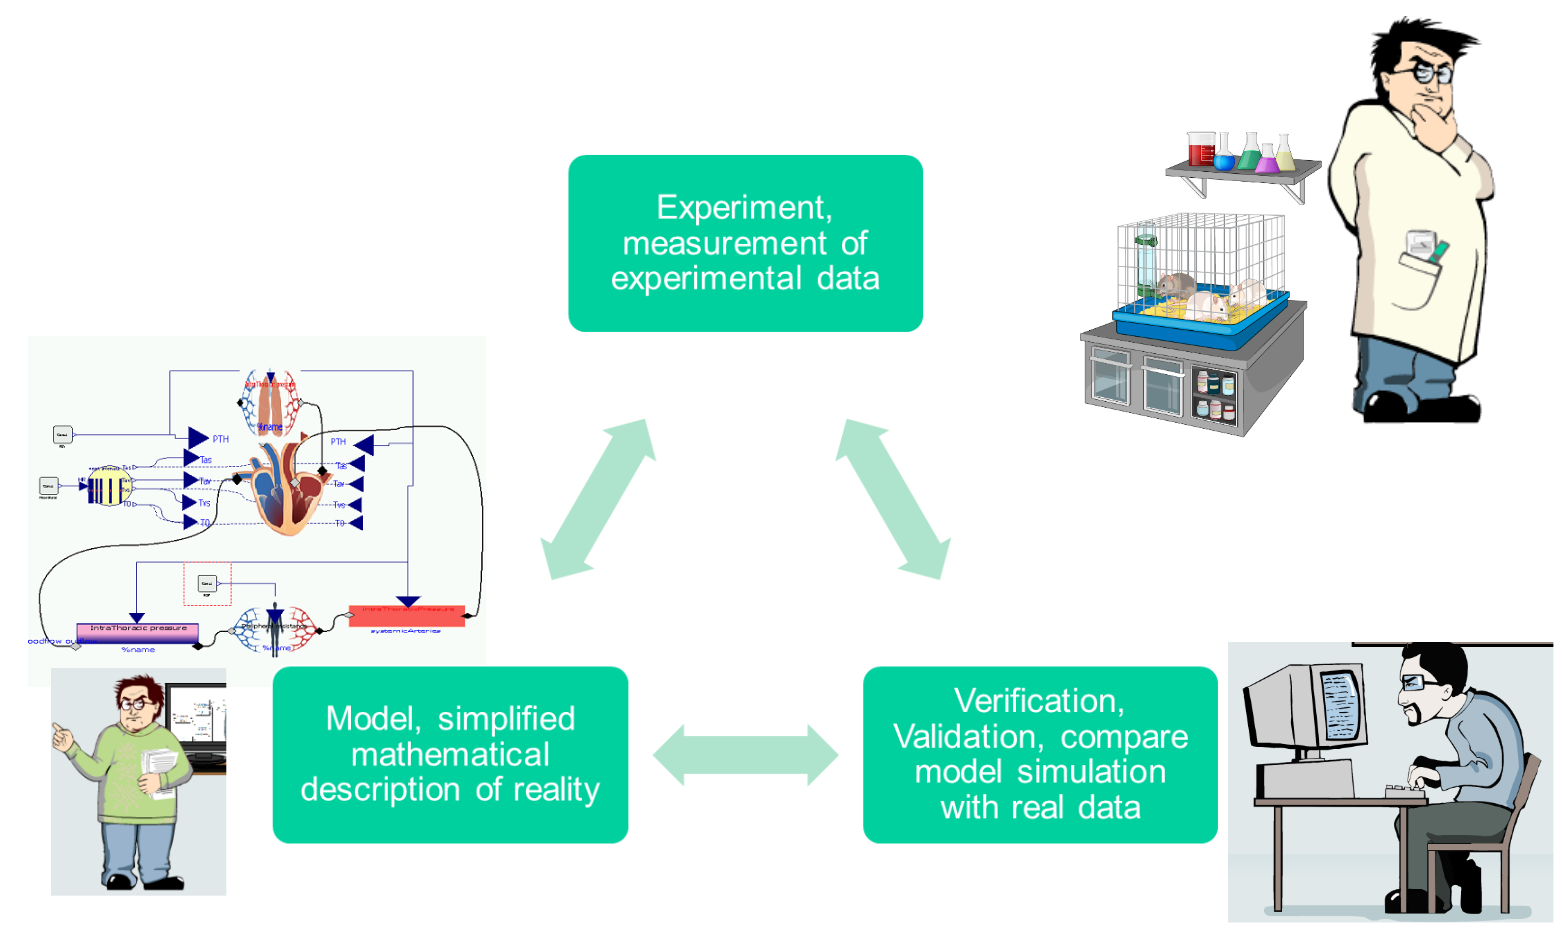
\includegraphics[width=1\textwidth]{chapter3/modeling.png}
    \caption{Schematic illustration of scientific process. The experiments produce data which are interpreted and a hypothesis is formalized as a model. Validation compares the model simulation with experiment, if model satisfies the criteria - is in agreement with real experiments, then the validated model can be used for other purposes.  %\bibentry{EGICompendium2013} \bibentry{egi2014}.
    }
    \label{fig:modeling}
\end{figure}

Application of the mathematical modeling techniques towards the biomedical research is sometimes called as systems biology approach combining the reductionism and integration as denoted by Kohl et al.\cite{Kohl2010}. Application towards the clinical practice include the quantification of the diagnostic index or treatment strategy and it is a goal to develop tools, database models and methods of several Physiome projects, e.g. VPH-Physiome project presented by Hunter et al.\cite{Hunter2009}.

One of the earliest complex and integrative modeling effort was a model of circulation and it's regulation published by Guyton et al. in 1972 \cite{Guyton1972} which via derivative and technological upgrade continues as "Human Model" or "HumMod" introduced by Hester et al. \cite{Hester2011systems,hester2011} with a focus on integration effort. Different approach of modeling human physiology is a database of smaller models focusing on some particular physiological phenomenon. E.g. the NSR Physiome project introduces  JSIM\footnote{JSIM: \url{http://www.physiome.org/jsim/} accessed January 2015} Java based simulation system to support modeling in  physiology. Repository of several hundred of models were published using this system \cite{Butterworth2014}. The similar effort is done by IUPS Physiome project and repository of models are  based on XML standard languages CellML and FieldML \cite{Hunter2004,Yu2011}. The Systems Biology Markup Language (SBML) is used for modeling biological system at the level of biochemical reaction and regulatory network and another database collects several hundreds of curated and non-curated models \cite{Hucka2004,LeNovere2006}.



%The methods and examples of modeling cardiovascular system are described in the next section \ref{sec:methodsmodels}. The methods of estimating parameters of complex models are described in section \ref{sec:methodsestimation} and particular results are described in section \ref{sec:resultsestimation}.

%\label{sec:results}
\subsection{Modeling methodology}
\label{sec:methodsmodels}
%For building complex models it seems that acausal (or declarative) modeling technique is key feature as it allows to express the variables declaratively, acausal modeling tool (e.g. Modelica or MATLAB\textsuperscript{\textregistered}  SIMSCAPE\texttrademark) figures out which are the dependent and independent variables upon compilation\cite{fritzson2002}. This allows building complex systems of equation from composed components and the model diagrams still captures the essence of the modeled reality much better and the simulation models are much more legible and thus also less prone to mistakes\cite{Kofranek2008,FernandezDeCanete2013}. 

The methodology of formalizing mathematical models is influenced by the abilities of underlying modeling language used. 
The Modelica language is an object-oriented, equation based and acausal modeling language standardized by Modelica association\footnote{\url{http://www.modelica.org} accessed February 2015}.
JSIM, CellML, SBML or HumMod are domain specific languages and the tools able to work with them are primarily developed within physiological or systems biological communities. Other authors use commercial or industry standard tools for mathematical modeling and computing. E.g. Kofranek et al. describes Guyton's 1972 model in MATLAB\textsuperscript{\textregistered} Simulink \cite{Kofranek2010} and the derivative HumMod in acausal object-oriented Modelica language \cite{Kofranek2011hummod,kofranek2013hummod}. Fernandez et al. describes models of cardiovascular pulsatile system using MATLAB Simscape  \cite{FernandezDeCanete2013} and recently in Modelica  \cite{FernandezdeCanete2014}.

Thus, there is an open debate whether in-house domain specific language and tools like JSIM, CellML and FieldML, SBML or HumMod reached its capabilities for representing complex models. Only the HumMod reached the integrative approach building the complex integrative model of human physiology using lumped parameter approach. I contributed to the idea of key features which involves acausal modeling technique and object orientation which keeps the complex model structure decomposed into understandable and maintainable parts and allows covering complexity of models like HumMod. 

%\emph{Object orientation} means that the definition of model is class as in object oriented programming, instance of the model is object,  each instance can share type and differ in parameters and the place where it is used, inheritance and some sort of polymorphism is possible.
%\emph{Equation based} means that the equation is not statement, thus the relation among variables can be expressed in any form and Modelica tool will decide which one is input and output upon compilation. %E.g. from the equation $q = \frac{dV}{dt}$ the process of computation can lead to $ q:= der(V)$ or $ V := \int{q}dt$ based on whether the $V$ or $q$ is known from the context.
%\emph{Acausal} connector is special purpose class to define variables of the model shared with other models or classes. Connecting two or more components via acausal connector will generate analogy of Kirchhoff's law: equality of all "non-flow" variables in connected connectors \begin{equation}p_1=p_2=\ldots =p_n\label{eq:kirchhoff1}\end{equation}
%and zero sum of all "flow" variables \begin{equation}\sum_{i=1}^n q_i=0\label{eq:kirchhoff2}\end{equation}
%
%To model e.g. cardiovascular system (CVS) we can decompose it to abstract component expressing hydraulic elasticity and hydraulic resistance. Connector \emph{HydraulicPort} with "flow" variable $q$ and non-flow variable pressure $p$ is presented in Modelica source code:
%\begin{lstlisting}[language=modelica]
%connector HydraulicPort
%  flow Real q;
%  Real p;
%end HydraulicPort;
%\end{lstlisting}
%Model of hydraulic resistor(conductor) with parameter $G$ denoting conductance and two hydraulic ports express the equations:
%\begin{equation}
%q_{in}.q = -q_{out}.q \label{eq:conductor1}
%\end{equation} 
%\begin{equation}
% q_{in}.q = G \times (q_{in}.p-q_{out}.p) \label{eq:conductor2}
%\end{equation}
%Model of hydraulic elastance with parameters $V_0$ as unstressed volume $p_0$ external pressure and $C$ compliance(reciprocal value of elastance) with state variable $V$ volume express these equation:
%\begin{equation} \label{eq:elastic1}p-p_0 = \left\{   
%  \begin{array}{l l} 0 & \quad \text{if } V \text{\textless} V_0 \\ 
%    \frac{V-V_0}{C} & \quad \text{otherwise}
%  \end{array} \right.\end{equation} 
%\begin{equation}\label{eq:elastic2}\frac{{\rm d}V}{{\rm d}t} =  q\end{equation} 
%Both models can be written in Modelica as:
%\begin{lstlisting}[language=modelica,multicols=2]
%model HydraulicConductor
%  parameter Real G;
%  HydraulicPort qin;
%  HydraulicPort qout;
%equation 
%  qin.q= -qout.q; // eq.(3.3)
%  qin.q = G*(qin.p-qout.p); // eq.(3.4)
%end HydraulicConductor;
%
%
%
%model HydraulicElastance
%    Real V;
%    parameter Real V0;
%    parameter Real p0;
%    parameter Real C;
%    HydraulicPort qin;
%equation 
%   // eq.(3.5)
%  qin.p-p0 = if (V<V0) then 0 else (V-V0)/C;
%  der(V) = qin.q; // eq.(3.6)
%end HydraulicElastance;
%\end{lstlisting}
%
%This can be used to model two ideal baloons with liquid  interconnected via a tube characterized by some resistance. The acausal connectors \emph{qin} and \emph{qout} are connected via the \emph{connect()} statement in the following listing:
%\begin{lstlisting}[language=modelica]
%model twoballons
%  HydraulicConductor systemicResistance;
%  HydraulicElastance arteries;
%  HydraulicElastance veins;
%equation 
%  connect(arteries.qin, systemicResistance.qin);
%  connect(systemicResistance.qout, veins.qin);
%end twoballons;
%\end{lstlisting}
%
%The concrete instances may differ e.g. in a way what is known of the system, either by external measurement, or by some superior model. The \emph{ballsVolume} is initialized with initial volume of first balloon \emph{V(start) = 5000}. But the model \emph{ballsFlowPressure} is initialized with initial pressure generated by the baloon \emph{p(start) = 2980.67}.
%\begin{lstlisting}[language=modelica,multicols=2]
%model ballsVolume
%  extends twoballons(
%    arteries(
%      V(start=5000),
%      V0=529,
%      p0=0,
%      C=1.5),
%    systemicResistance(G=1),
%    veins(
%      V0=2845,
%      p0=0,
%      C=200));
%end ballsVolume;
%model ballsPressure
%  extends twoballons(arteries(
%      V0=529,
%      p0=0,
%      C=1.5,
%      qin(p(start=2980.67, fixed=true))),
%    systemicResistance(G=1),
%    veins(
%      V0=2845,
%      p0=0,
%      C=200));
%end ballsFlowPressure;
%\end{lstlisting}
%Based on an concrete instance of the model with specific initial condition, the Modelica tool will decide what will be dependent and  what independent variables and computation flow based on the above rules and equation is generated as in following statements with assigning symbol (\emph{:=}).
%\begin{lstlisting}[language=modelica,multicols=2]
%// Translated M. model generated by Dymola  
%//  ballsVolume
%
%
%
%// Dynamics Section
%  systemicResistance.qout.p := veins.p0+
%    (if veins.V < veins.V0 then 0 
%    else (veins.V-veins.V0)/veins.C);
%  systemicResistance.qin.p := arteries.p0+
%    (if arteries.V < arteries.V0 then 0
%    else (arteries.V-arteries.V0)/arteries.C);
%  der(arteries.V) := systemicResistance.G*
%    (systemicResistance.qout.p-
%      systemicResistance.qin.p);
%  der(veins.V) :=  -der(arteries.V);
%
%
%
%// Translated M. model generated by Dymola 
%// ballsPressure
%// Initial Section
%...
%// Dynamics Section
%  systemicResistance.qout.p := veins.p0+
%    (if veins.V < veins.V0 then 0 
%    else (veins.V-veins.V0)/veins.C);
%  arteries.qin.p := arteries.p0+
%    (if arteries.V < arteries.V0 then 0 
%    else (arteries.V-arteries.V0)/arteries.C);
%  arteries.qin.q := systemicResistance.G*
%    (systemicResistance.qout.p-
%      arteries.qin.p);
%  der(veins.V) :=  -arteries.qin.q;
%  der(arteries.V) := arteries.qin.q;
%\end{lstlisting}
%

%
%Empirically derived function of flow rate per time going out from the heart:
%\begin{equation} \label{eq:heart} q = \left\{   
%  \begin{array}{l l} 0 & \quad \text{otherwise} \\ 
%    \sin \left( 
%    \frac{t_c-T_{D1} }{ T_{D2} -T_{D1} } * \pi \right) * Q_{peak} 
%    & \quad \text{if } t_c \in (T_{D1}..T_{D2})
%  \end{array} \right.\end{equation} 
%\begin{equation}\label{eq:flowrate2}\frac{{\rm d}V}{{\rm d}t} =  q\end{equation} 
%
%\begin{lstlisting}[language=modelica]
%model HeartFlow
%  HydraulicPort qout;
%  discrete Real T0, HP=0.8;
%  Boolean b(start = false);
%  parameter Real TD1 = 0.07, TD2=0.39, QP = 0.000424;
%  Real tc "relative time in cardiac cycle";
%equation
%  b = time - pre(T0) >= pre(HP) "true if new cardiac cycle begins";
%  when {initial(), b} then
%    T0 = time "set begining of cardiac cycle";
%  end when;
%  tc = time - T0 "relative time in carciac cycle";
%  qout.q=if tc>TD1 and tc<TD2 then sin((tc-TD1)/(TD2-TD1)*Modelica.Constants.pi)*QP else 0;
%end HeartFlow;
%\end{lstlisting}

The paper \cite{Kulhanek2014Modeling} \emph{Modeling of Short-term Mechanism of arterial pressure in the cardiovascular system: Object-oriented and acausal approach} in Appendix~\ref{app:modeling} published disputation about causal and acausal approach in using Modelica for modeling pulsatile cardiovascular system (CVS)\nomenclature{CVS}{cardiovascular system} and possible enhancement for more complex models. 

The paper \cite{Kulhanek2014mefanet} \emph{Simple Models of the Cardiovascular System for Educational and Research Purposes} in Appendix~\ref{app:simplemodelsd} published detailed methodology of modeling lumped parameter pulsatile CVS in Modelica. 

Common guide to the Modelica language and it's capabilities are in the book of Fritzson \cite{fritzson2002} or in the on-line book by M.Tiller \cite{Tiller2014}.


\subsection{Identification of physiological systems}
\label{sec:estimation}

%\subsection{Identification of physiological systems}
%Model verification (whether simulation of the model shows desired behavior) and model validation (whether model simulation agrees with new observation of real system) are important steps in system analysis and model construction. 
Usually some knowledge of the system - the structure is available and unknown coefficients (parameters) remain unknown. Once the model is formalized and constructed, further problem is to estimate the model parameters so that the model reproduces real world system. This procedure is sometimes called system identification and the objective of parameter estimation is usually to minimize the following function (to find least squares of the differences between predicted and measured values):
\begin{equation} \label{eq:parameter} 
f( \vec{p} ) = \sum_{i=1}^{n} ( M(t_{i},\vec{p} ) - d(t_{i}) )^2 \to min  
\end{equation} 
where $\vec{p}$ is vector of values of parameters, $M(t_{i},\vec{p})$ is model simulated at time $t_{i} $ with the given parameter values $\vec{p}$ and $d(t_{i})$ is the measured experimental value at time $t_{i}$. 
In general mathematical models of biological systems are in most cases non-linear and some of them are non-differentiable, therefore global optimization methods must be used. Algorithmically, the problem of parameter estimation was shown to belonging to the \emph{NP-complete} problems \cite{Hofmann2005} which implicates that current exact algorithm is brute force search -- trying all possible values of parameters and simulate the model with them and find minimum of the objective function \ref{eq:parameter}.
Further reading about parameter estimation and system identification can be found in book edited by Eykhoff \cite{Eykhoff1981} or book of Khoo \cite[p.~159]{khoo2000}.

The heuristic methods (evolution strategies), randomization methods (Monte Carlo) and others can be used to find at least some solution in a reasonable time. The evolution strategies were identified as robust with potential to utilize parallel computing as shawn by Moles at al.\cite{Moles2003}

%However, exact solution may not be needed because the models itself are by definition approximation of real system, and the input data are measured with some degree of error. 

Parameter estimation and further analysis methods are part of specialized mathematical software. E.g. Pruet et al. used Metropolis algorithm to produce a distribution of parameters to calibrate the model of human cardiovascular physiology, which were further tested against predictive ability of circulatory failure and statistical methods of the software Wolfram \textit{Mathematica} were used \cite{Pruett2013}. The iterative improvement method in the software MATLAB Simulink\textregistered ~was used in estimating 2 parameters of simple cardiovascular model by Takahashi et al. \cite{Takahashi2013}. Several methods were compared in estimating multiple parameters of cardiovascular system in MATLAB Simulink\textregistered ~by Abbass et al. \cite{Abbass2012}.

Maffioletti et al. published GC3Pie framework utilizing evolutionary algorithms and introduced workflow to identify parameters of models for economical predictions using grid computing \cite{maffioletti2012computational}. Humphrey et al. calibrated hydrology models utilizing commercial Windows Azure cloud computing infrastructure with a significant speedup on the modified dynamically dimensioned search algorithm\cite{Humphrey2012,Tolson2007}. 

%Selected methods to estimate parameters are introduced in section \ref{sec:methodsmodels}. 

%As already identified also by other authors of some calibrating systems, the parameter estimation is used sporadically, however, with high demand of computational task in temporal time. Thus, I proposed and designed the system which can distribute the simulation task into grid-computing and cloud-computing infrastructure and the computational capacity can be provisioned on-demand. % this brings significant speedup for parameter estimation of complex model but limited speedup on simple models. 


\subsection{Methods for Parameter Estimation}
\label{sec:methodsestimation}

\begin{figure}[htb]
    \centering
    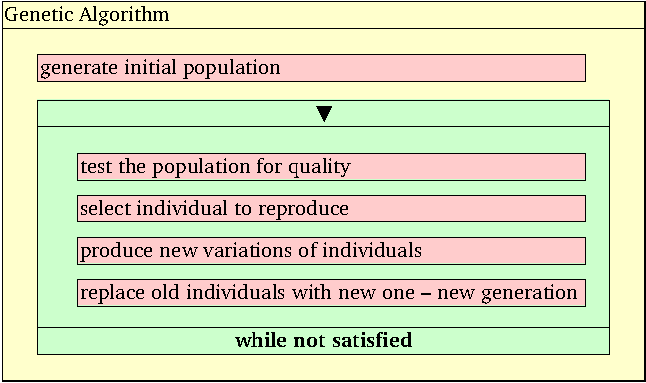
\includegraphics[page=1]{chapter3/GA-kopenogram-crop.pdf}    
%    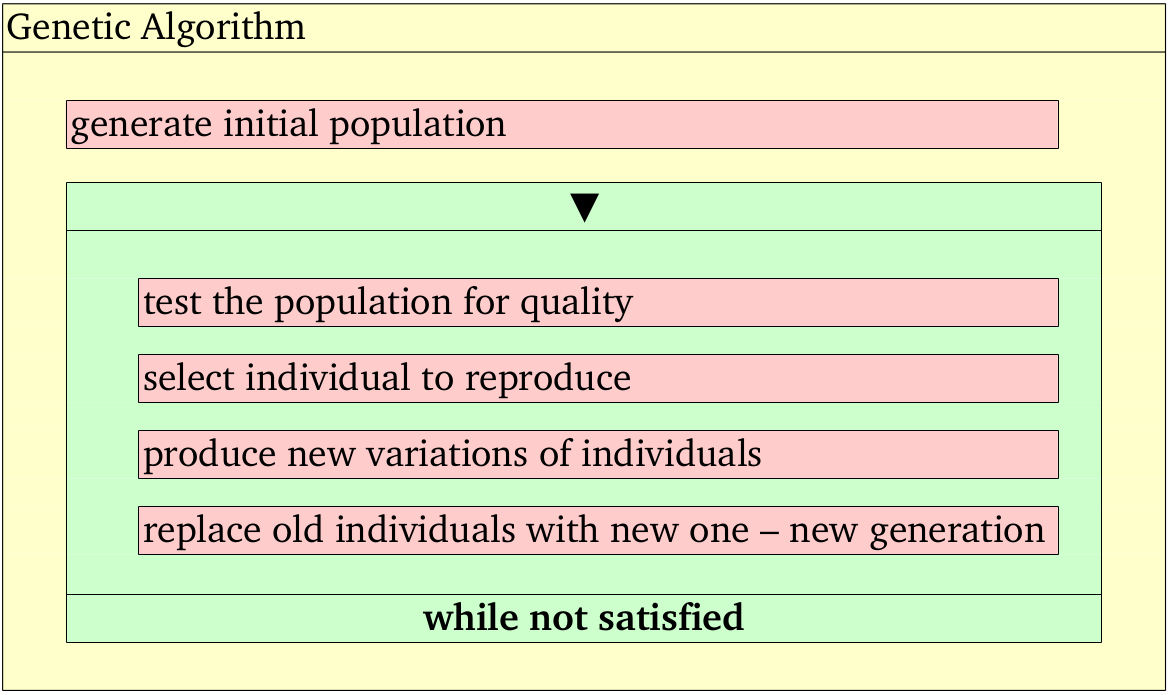
\includegraphics[width=0.5\textwidth]{chapter6/GA-kopenogram.png}
    \caption{Kopenogram of genetic algorithm. 
    }
    \label{fig:GA-kopenogram}
\end{figure}

Evolutionary algorithms can be used as heuristic strategy for finding global minimum or maximum and it can be used to estimate the parameters of the model. Genetic algorithm a type of evolutionary algorithm which encodes individuals as binary string was introduced e.g. by Holland\cite{Holland1975} and the algorithm steps are schematically presented in figure \ref{fig:GA-kopenogram}.

\begin{figure}[htb]
    \centering
    \includegraphics[page=2]{chapter3/GA-kopenogram-crop.pdf}    
%    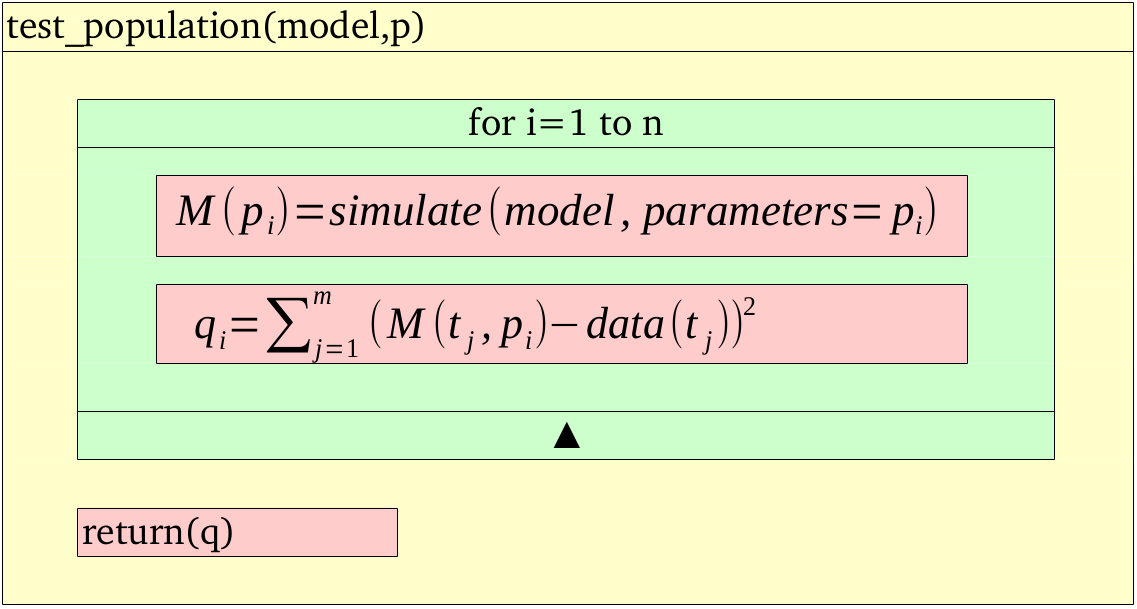
\includegraphics[width=0.5\textwidth]{chapter6/GA-kopenogram2.png}
    \caption{Kopenogram of genetic algorithm and specific test of the population for quality in case of parameter estimation. Model is simulated according to individual $i$ with parameters $p_i$ and the quality $q_i$ is counted per the objective function \ref{eq:parameter}.
    }
    \label{fig:GA-kopenogram2}
\end{figure}

The iteration within the loop "$\blacktriangledown \ldots$ \emph{while not satisfied}" depends on previous iteration, thus it cannot be parallelized.
The step \emph{test the population for quality} has algorithmical structure in fig.\ref{fig:GA-kopenogram2} for parameter estimation tasks. Each iteration in the loop "\emph{for i=1 to n}" is independent therefore loop parallelism (section \ref{sec:parallelprogramming}) can be utilized and implemented here.

%The Amdahl's law in equation \ref{eq:amdahl} can be used to estimate  the theoretical speedup limitation for the specific model and potential gain for identifying different types of models can be stated. We assume that the simulation of the model with any parameters will take the same time, even this is not generally true as the non-linear models and numerical methods may cause different steps to be performed for different parameter values. 

%The specific fraction $\alpha$ for the model determines the level of scalability of the model within the parallelized system. For the complex models the $\alpha$ will decrease. The specific estimates of the fraction $\alpha$ and it's influence on the scalability and results are presented in section \ref{sec:resultsestimation}.

\subsubsection{Architecture of system for parameter estimation}
\begin{figure}[hbt]
    \centering
     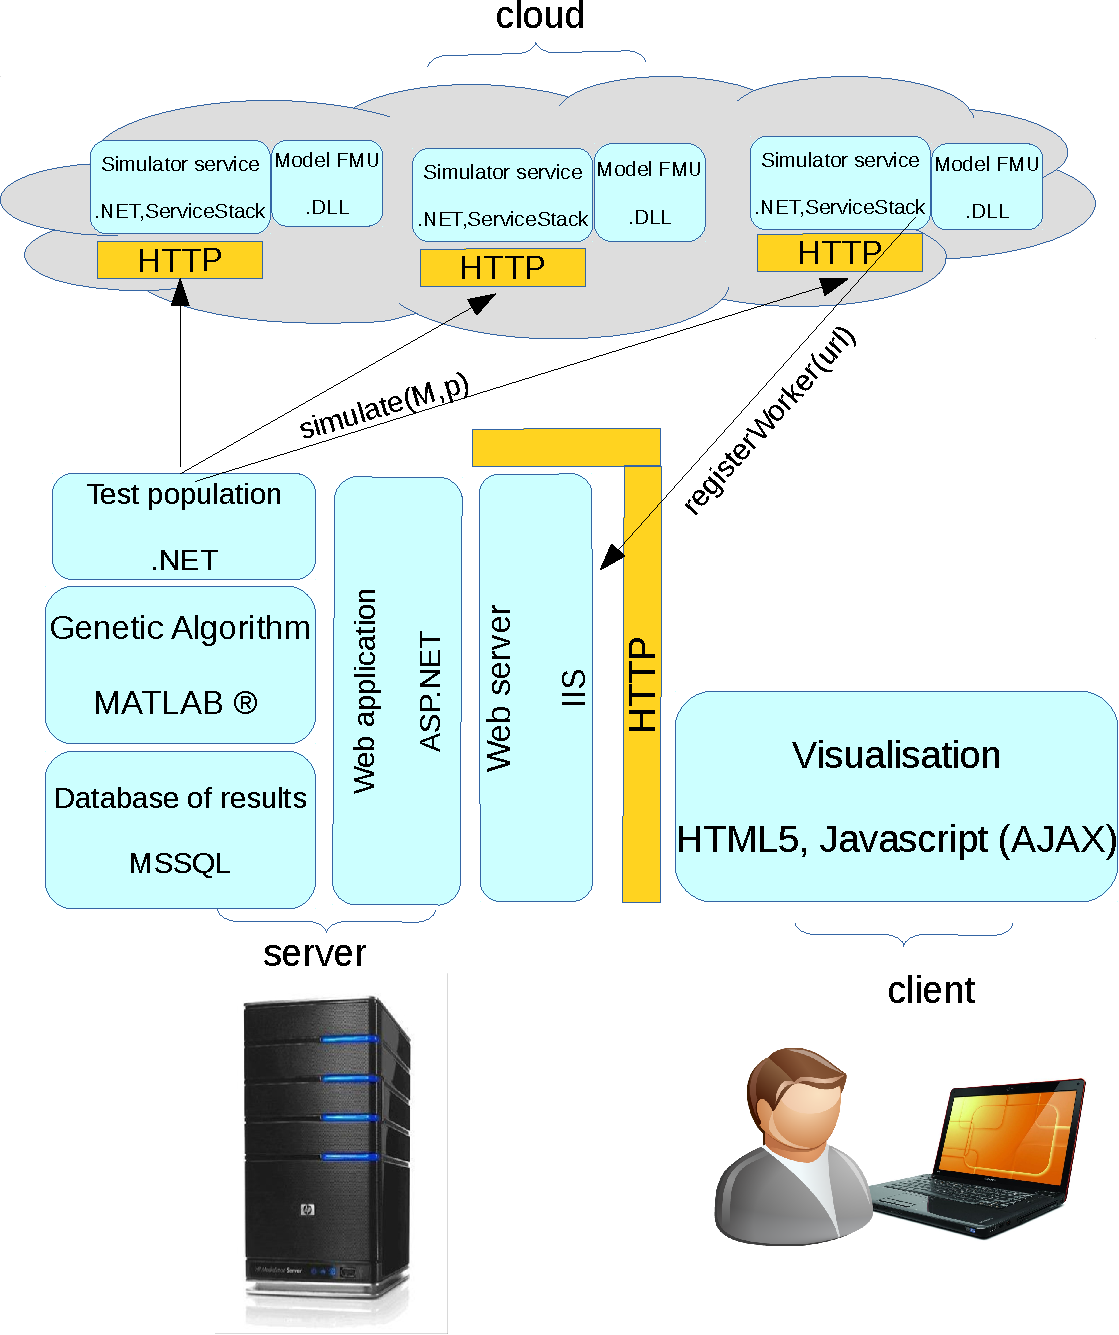
\includegraphics[page=1,width=0.75\textwidth]{chapter3/architekturaestimation-crop.pdf}  
    \caption{Architecture of the system employing genetic algorithm and distributing the task \emph{simulate} into cloud computing environment.}
    \label{fig:architectureestimation}
\end{figure}
Proposed architecture of the system for parameter estimation (fig. \ref{fig:architectureestimation}) was influenced by the need of some interactivity and overall accessibility for users which is fulfilled by the web UI. The key part of the system in opposite side is a model exported into a binary platform dependent library. 
The specific model of a studied system implemented in Modelica is exported into standard Functional Mockup Unit(FMU)\nomenclature{FMU}{Functional Mockup Unit}  which is standardized XML\nomenclature{XML}{Extensible Markup Language} metadata packaged together with  binary library .DLL (or .SO) following standardized API \cite{Blochwitza}\footnote{\url{https://www.fmi-standard.org/} accessed February 2015}. In the time of writing the thesis the most stable Modelica tool export was Dymola\footnote{\url{http://www.dynasim.se} - Dymola tool, accessed March 2015} export to FMU for MS Windows platform. 

The parallelization is implemented using threads in \emph{test\_population} method which within a loop follows fork/join pattern -- the created threads simultaneously asks for simulation results with a parameter set and main process waits until all results are returned to compute full vector of quality evaluation $q$.

Packaged with .NET ServiceStack framework\footnote{\url{https://servicestack.net/} accessed February 2015} it exposes a simulation functionality as a RESTful web service which can be accessed and orchestrated by the \emph{test\_population} algorithm. The implementation of genetic algorithm is reused from MATLAB \texttrademark and with a database of results in a SQL database is integrated with ASP.NET web application presenting a web user interface and functionality to a user.
The result of applying the methods and deploying the designed system in local cluster and cloud computing infrastructure is described in section \ref{sec:resultsestimation}.

\subsection{Parameter Sweep}
\label{sec:sensitivity}
After the parameter estimation a further problems arise with structural identifiability and analysis of sensitivity to the estimated parameter values\cite[p.~176]{khoo2000}. 

\begin{figure}[hbt]
    \centering
     \includegraphics[page=4]{chapter3/GA-kopenogram-crop.pdf}    
%    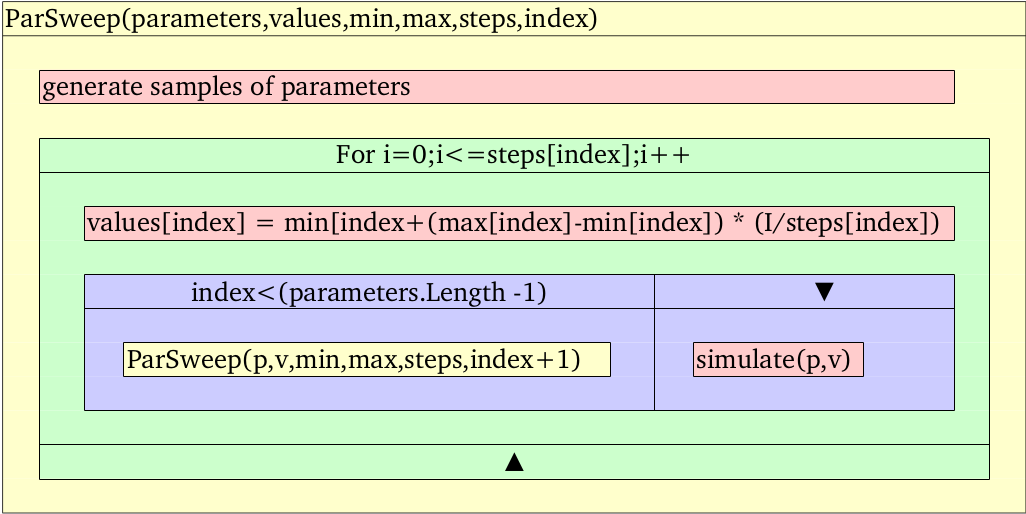
\includegraphics[width=1\textwidth]{chapter3/paramsweepkop.png}
    \caption{Kopenogram of recursive parameter sweep algorithm. $p$,$v$,$min$,$max$ and $steps$ are arrays with the same dimension holding parameter name, value, starting and stoping value and number of steps which needs to be performed between starting and stopping value per each $index$.    
    }
    \label{fig:paramsweep}
\end{figure}

Parameter sweep (PS) is one of the techniques used for sensitivity and uncertainty analysis which is based on changing selected parameters and simulating whole model and quantifying the change on model behavior with different parameters. Uncertainty and sensitivity analysis tries to determine how a change of the value of parameter will contribute to the model output and how the estimation of parameter values are robust to errors of measurement of the real data. Various methods to do uncertainty and sensitivity analysis can be found e.g. in a reviews by Helton et al. \cite{Helton2006} or a books by Saltelli et al.\cite{Saltelli2004,Saltelli2008}. 

Recursive algorithm of parameter sweep for exploring parameter space (in fig.\ref{fig:paramsweep}) generates tremendous number of simulation. Presuming that \emph{simulate} operation takes constant time for any parameters (which is not true in general) the time complexity of PS is $O(\prod_{i=1}^{n}) \text{steps}_i) \approx  O(k^n)$ where $k=\max_{i=1}^n(\text{steps}_i)$ and $n$ is number of parameters to be swept. E.g. for 1000 values for each parameter: $O(1000^n)$. The large number of distinct simulation can take tremendous time on single computer. However, in contrast to parameter estimation, each of the simulation is independent and PS algorithm is determined as embarrassingly parallel and is implemented in many grid-computing projects and workflows e.g. P-Grade portal as published by Kacsuk et al.\cite{Kacsuk2011}.

To perform parameter sweep algorithm on the models of human physiology in Modelica language an export from the Modelica is needed. The FMU standard supported by many tools exports FMU as 

a BOINC platform\cite{Anderson2004}\footnote{\url{http://boinc.berkeley.edu/} accessed February 2015} is customized following the task parallelism and master/worker programming model (mentioned in section \ref{sec:parallelprogramming}). The Modelica model exported as FMU for Windows platform is integrated with BOINC wrapper and as a whole it is integrated into BOINC platform deployed on a server as seen in fig. \ref{fig:paramsweeparch}. 

\begin{figure}[htb]
    \centering
     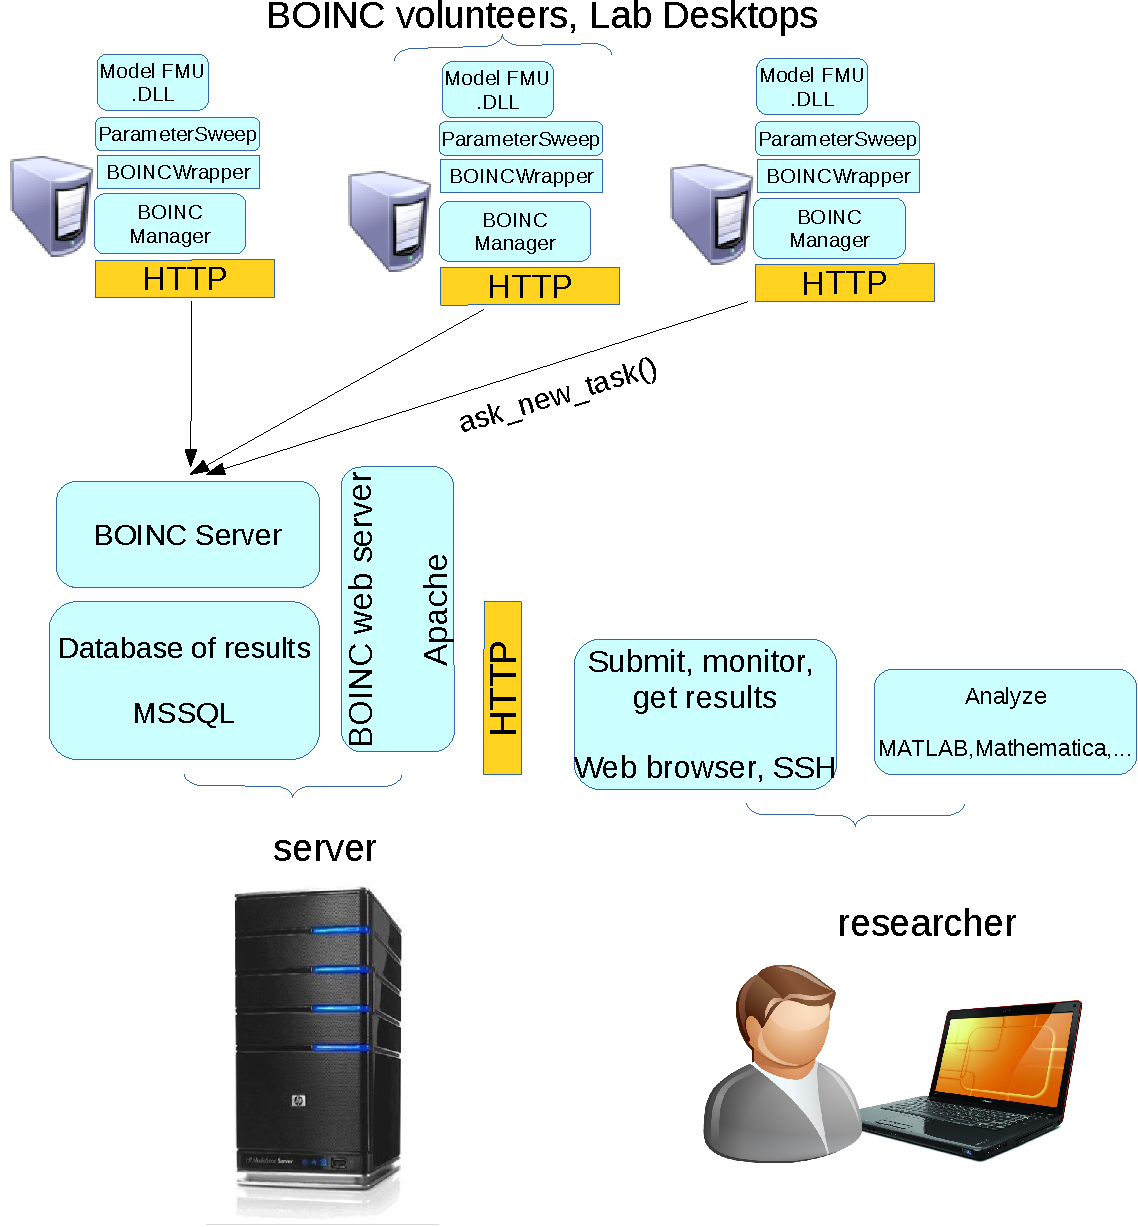
\includegraphics[page=1,width=0.75\textwidth]{chapter3/architekturaparamsweep-crop.pdf}    
%    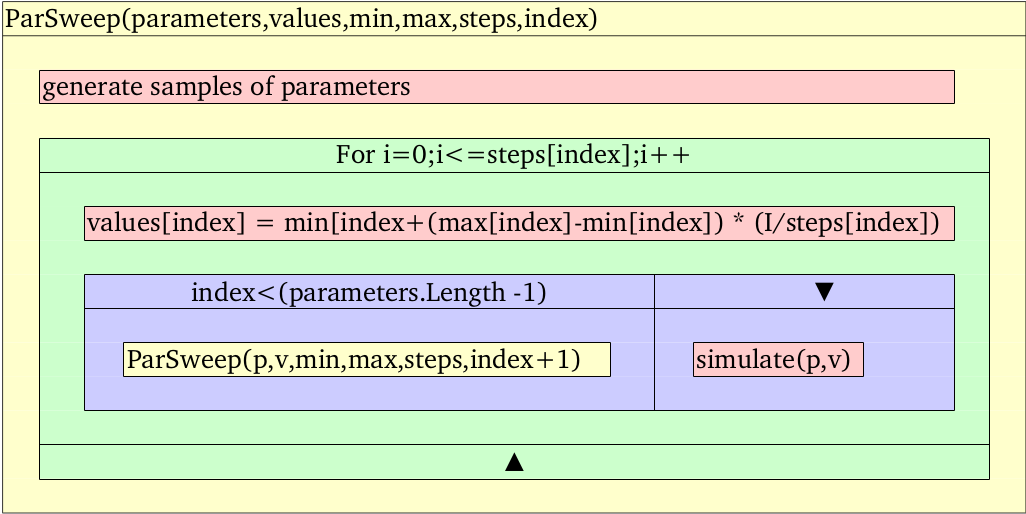
\includegraphics[width=1\textwidth]{chapter3/paramsweepkop.png}
    \caption{Architecture of parameter sweep application. The whole parameter space is divided into smaller spaces which are resolved by the BOINC workers}
    \label{fig:paramsweeparch}
\end{figure}

The results are described in section \ref{sec:resultsestimation}.

%The paper \cite{Kulhanek2011} \emph{From Educational Models Towards Identification of Physiological Systems} in Appendix~\ref{app:fromeducational} describes desktop grid system BOINC and deployment for parameter estimation mentioned in previous chapter. However, per the high latency of BOINC solution, the of the specific Modelica model exported into Windows executable into BOINC client. 

%\chapter{Sharing medical images}
\label{sec:imaging}
%\label{sec:medicalapp}
This chapter introduces acquiring, storing and sharing digital medical images and related metadata within hospital or healthcare provider and among them and research institution.

%are covered in section \ref{sec:introimages}. Overview of analysis of speech and voice and it's relation to voice science is in section \ref{sec:introvoice}. Overview of models and simulation of human physiology and it's relation to systems biology is briefly covered in section \ref{sec:intromodels}.


%The computing in biomedicine can be divided into research and clinical application. %Translational science aims to "translate" findings from research to better health care including diagnostic tools, procedures, drugs, etc.

%In case of research use-cases, processing medical information helps to make more precise current theories or support formulating new one. In case of clinical use cases, processing medical information helps to analyse and interpret the information, predicting future trends and support decision on some intervention.

%\footnote{Motivation of using distributed computing technologies is to share physical data, among multiple organizations, where there is no need or other barriers to store all data centrally, e.g. for legal or capacity limitation. A lot of medical information within biomedical research came from real patient and such information are protected by some regulation and processing of them is regulated and controlled by the country laws or international agreements. Thus there must be considered ethical as well as legal issues how to deal with such information. Sharing and processing of medical images are covered in section \ref{sec:introimages}. Providing access to services with high values is another motivation of using distributed computing technologies. E.g. basic and advanced analysis of biological signals, especially of voice is described in section \ref{sec:introvoice}.}


Digital medical images involves the image acquisition, preprocessing, storing and searching.
Clinicians use patient image mainly for visualization and diagnostic purposes. Computer assisted methods facilitate the diagnostic process and involves image enhancement (to reduce image noise and increases the contrast), image segmentation (to separate different types of structures from background and from each other), quantification methods (to determines the structure shape, size, volume), registration methods (to process and join multiple different images into one).
Comprehensive concepts and digital techniques are presented e.g. in book edited by I.N.Bankman\cite{Bankman2000}.

Acquisition of the medical image is covered with different modalities (different types of equipment and sensors) by radiologists or other specialists. DICOM\footnote{DICOM: \url{http://dicom.nema.org/} accessed January 2015} format and standard becomes most popular to exchange medical images electronically and picture archiving communication systems (PACS) are currently parts of information systems in hospitals.

\begin{figure}[ht]
    \centering
    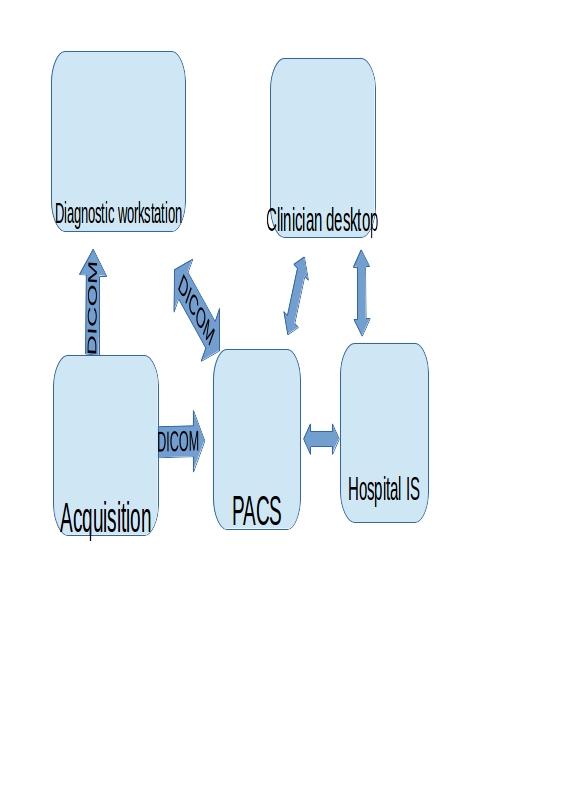
\includegraphics[width=0.8\textwidth, height=8cm]{chapter4/pacs.png}
    \caption{Typical workflow of medical image in hospital. Data acquisition is made by modalities (magnetic resonance, ultrasonography, X-ray radiography, etc.) and using DICOM format and protocol it can be directly transferred and visualized by diagnostic workstation. With metadata filled by an expert physician the image is stored in PACS. Other desktops within hospital can retrieve the image and review the report. The hospital information system may be involved in other workflows and communicate with other formats and standards (HL7,...)
    }
    \label{fig:pacs}
\end{figure}

As the data processed in hospital information systems contains sensitive information of real patients, these are protected and processing and storing is regulated by the national or international laws or agreements.
Development of telecomunication and network technologies a enabled telemedicine -- providing healthcare over remote distance. It requires to share and exchange  sensitive data of real patient among different helthcare providers and additionaly such data may be very valuable for further research. Security and encryption should be addressed and DICOM standard itself doesn't solve security issues appropriately, thus encyption during transferring the data over computer network must be ensured by other techniques.

In the Czech Republic, there exists several projects in production interconnecting different hospitals, clinics and other healthcare organization to exchange medical images. Project ePACS allows interconnecting each participant's PACS system via dedicated VPN channel to the central node and exchange of medical images are realized by routing the data flow from one VPN channel to the other\footnote{ePACS:\url{http://www.epacs.cz}, accessed January 2015}. Another approach is used in the project MEDIMED held by Masaryk University in Brno. Instead of dedicated VPN channel, they use  SSL encryption over standard TCP/IP communication and regional hospitals and healthcare providers are interconnected via the MEDIMED servers \cite{Slavicek2010,Zatloukal2012}.% \cite{Javornik2011,Zatloukal2012}.
In other countries, there were tested cross-border teleradiology in projects Baltic e-health, R-Bay and others \cite{Ross2010,Saliba2012}.
These projects are focused on sharing the medical images and other knowledge and information.

Storing the sensitive medical information is usually done in some trusted environment, e.g. in secured server or cluster owned by a trusted institution or within the hospital. In case of using distributed technologies, this lead to an idea to move and facilitate deployment of the grid services storing medical data to the institution which has been acknowledged to store them using e.g. pre-installed virtual machines as a sealed grid \cite{Kuba2007a}.

Additionaly for the research purposes an access to the wide range of medical images is needed for provenance, for research of new processing and diagnostic methods, etc.  DICOM records can be "deidentified" or anonymized for research purposes to protect sensitive personal data, but keep important information for research purposes. The Globus MEDICUS project published by Erberich et al.\cite{Erberich2006,Erberich2007} is based on Globus Toolkit middleware to federate clinical and research application via a grid-computing infrastructure. It  introduces a new DICOM Grid Interface Service for DICOM compliant devices and application based on Pixelmed Java DICOM Toolkit\footnote{\url{http://www.pixelmed.com/} accessed February 2015}. Currently the project is hibernated since 2008 and no further development was published\footnote{\url{https://dev.globus.org/wiki/Incubator/MEDICUS} accessed February 2015}. Similar effort was done with a project Medical Data Manager which uses gLite grid middleware by Duque, Montagnat et al.\cite{Duque,Montagnat2007} \footnote{\url{http://modalis.i3s.unice.fr/softwares/mdm/start} accessed February 2015} or MediGRID project by Krefting et al.{Krefting2009,Krefting2010}. These project focuses not only on sharing medical images and knowledge, but also on processing them using grid computing technologies\cite{Krefting2010}.

%When we look to the architecture of the systems of sharing medical images the problematic part within the point-to-multipoint architecture is the central part of the systems already in production e.g. in Czech Republic (MEDIMED, ePACS). This may become single point of failure and bottleneck.

To summarize this section, digital medical image acquisition, store, exchange and processing became common in the past years and is currently using distributed computing techniques. There are several efforts to implement medical data management within grid or cloud infrastructure for research purposes and integrate them with the production infrastructures. Security is solved by authentication, authorization mechanism as well as by encrypting the data and/or anonymizing them to keep minimal information useful for research. Thus there is another question, how easily the previously mentioned grid-based technologies can be integrated with current distributed systems used to integrate hospital PACS. The following section \ref{sec:methodsimages} describes methods used to integrate a pilot deployment of Globus MEDICUS with current regional system for exchanging medical images - MEDIMED. The realization and other promising particular results are described in section \ref{sec:resultsimages}.

\section{Methods to share medical images in grid}
\label{sec:methodsimages}

The integration strategies based on standard protocol integration and client server architecture is used to integrate Globus MEDICUS with some local PACS system. Globus MEDICUS \cite{Erberich2006,Erberich2007} implements a DICOM Grid Interface Service (DGIS) which in one side communicate using DICOM protocol, and implements other services which stores metadata and location of replicas of the data using standardized Globus toolkit middleware. DGIS behaves as a gateway to this grid infrastructure and is usually installed on the location of integrated third party system; hospital PACS, workstation PACS client or DICOM modality communicate with DGIS using DICOM protocol.
To present DICOM studies The integration strategy based on shared database or files can be used to present the DICOM studies via web portal. Additionally the web portal might generate specific DICOM queries to DGIS.

The paper \cite{kulhanek2009}  \emph{Processing of Medical Images in Virtual Distributed Environment} in Appendix \ref{app:a} published details about the integration of Globus MEDICUS instance with MeDiMed project with a conclusion that the integration via DICOM protocol is almost seamless. The paper \cite{Kulhanek2008Mefanet} presented additional portal integration with DICOMViewer, which can provide access to the DICOM studies available in the Globus MEDICUS infrastructure.


\section{Results}
\label{sec:resultsimages}
The pilot grid infrastructure was established in the location of First Faculty of Medicine, Charles University in Prague, Central Military Hospital in Prague and CESNET association. And the Globus Toolkit middleware and Globus MEDICUS implementation was installed on linux based virtual machines using XEN hypervisor providing pilot services to access this grid based PACS system.



%\chapter{Voice Science}
\label{sec:voice}
With introduction of objective data analysis and laryngoscopy methods the voice science emphasized the cooperation among  laryngologist, speech pathologist and voice teacher.
The human voice ranges from 50 Hz to something about 1000 Hz, but there are large  individual variation. For analysis of digitally recorded voice, either habitual or singing, the Discrete Fourier Transformation(DFT) is used to produce frequency and amplitude analysis of recorded input voice samples. One of the most used class algorithm to compute DFT is class of Fast Fourier Transformation with computational complexity $O(n \log(n))$ \cite{Cooley1965,Frigo2005} and parallel version of the algorithms may introduce additional speedup for larger samples of analyzed data \cite{Gupta1993,Takahashi2003}. The result of analysis can be visualized in a voice range profile and there can be seen significant difference between untrained and trained voice as well as quantitatively seen some disorders  \cite{DeLeoLeBorgne2002,wuyts2003effects}.

Other methods to analyse vocal chords is laryngoscopy. The videostroboscopy and high speed video in laryngoscope methods produce video for analysing the real movement of vocal chords. The videokymography method introduced by Švec et al. complements the videostroboscopy and allows to visualize and analyze movement of vocal cords recorded by high speed camera on standard TV or monitor with an artificial image built from recorded sequence of selected section \cite{Svec1996,Svec2007}. 

In case of recorded sound and further analysis there is a question about how such a service can be integrated in grid-computing or cloud-computing environment to provide access to a complex application for non-technical voice specialists. Additionally, the analytical software was already developed and calibrated for selected sorts of microphones in MS Windows platform \cite{Fric2007,Fric2012}. Therefore I proposed and implemented a method that provides access to the analytical software remotely. The section \ref{sec:methodsvoice} describes how the analytical software was customized with a remote desktop protocol (RDP). Results are described in section \ref{sec:resultsvoice}. Similar approach might be used for processing the video recordings from laryngoscope, however, the practical limits are discussed in section \ref{sec:conclusion}. 


\section{Methods for remote analysis of human voice}
\label{sec:methodsvoice}
%One method to provide access to specialized service is via remote access protocols. Secure Shell (SSH) is used to establish secure channel via unsecured network (e.g. the Internet) from SSH client to SSH server providing e.g. remote command-line, remote command execution etc. It is one of the basic method to access the grid infrastructure and submit computational jobs. 
%Another method is to have a web portal and this web portal based on user's input executes command-line batch scripts over SSH, or it can utilize web services to submit computational job.
Terminal access to some remote computational capabilities, e.g. remote command-line or remote execution is another integration strategy to some remote infrastructure. Secure Shell (SSH) is used to establish secure channel via unsecured network (e.g. the Internet) from SSH client to SSH server and it is basic method to access grid-computing infrastructure. 

Remote Desktop Protocol(RDP) is a proprietary protocol for desktop sharing developed primarly in Microsoft Windows platform, however, today clients and servers exists for several other platforms. Next to remote command-line, remote execution it allows to access remote graphical desktop environment. %VNC is sharing protocol to access remote graphical desktop environment\cite{Richardson1998}. 
The software for parameterized Voice Range Profile (ParVRP) and Voice Range Profile in Real time (RealVoiceLab) was already developed and calibrated for selected sorts of microphones in MS Windows platform by Fric et al.\cite{Fric2007,Fric2012}. The implementation is done in MATLAB environment utilizing Signal Processing Toolbox\footnote{\url{http://www.mathworks.com/products/signal/} accessed February 2015}and compiled with MATLAB Compiler and distributed as an executable.

Instead of migrating the application into some compatible platform for grid-middleware, a virtual machine was introduced and access to the software is provided via RDP protocol. RDP itself contains redirection of several services, e.g. sound recording or drive access. Because the default sound recording redirection introduces some sound degradation without control, I proposed, implemented and integrated the custom RDP plugin with the ParVRP and RealVoiceLab software to redirect the sound recording without loss of information. 

The computation of frequencies and amplitude from the recorded samples utilizes Fast Fourier Transformation which has time complexity $O(n\log(n))$. Thus the computational complexity and theoretical speedup is not primary reason for making such application distributed. 

This type of application can be packaged as virtual machine template and configured within different types of cloud infrastructures and together with a script or web portal the on-demand deployment can be automated.

\section{Results}
\label{sec:resultsvoice}

The paper \cite{kulhanek2010b} \emph{Remote Analysis of Human Voice--Lossless Sound Recording Redirection} in the Appendix~\ref{app:bio} published technical details and results of such implementation.

Additionally the custom RDP plugin with the ParVRP and RealVoiceLab software to redirect the sound recording without loss of information was packaged as a virtual machine template and  deployed in the pilot virtual infrastructure next to the test instance of Globus MEDICUS.

The virtual machine template was also deployed to different cloud computing infrastructures. One to the Amazon EC2\footnote{\url{http://aws.amazon.com/ec2/} accessed February 2015} and second to the pilot scientific cloud launched in the begining of 2012 --MetaCloud\footnote{\url{http://www.metacentrum.cz/en/cloud/} accessed February 2015}.

 A comparison of these two was presented to the users and staff of CESNET and EGI in EGI Technical Forum 2012\cite{Kulhanek2012a} with focus on providing such science as a service.
 
%\chapter{Computational physiology}
\label{sec:models}
A mathematical formalization of the fundamental knowledge and relation among biological system - mathematical model - is used as a base abstraction to utilize current discoveries of the genomics and proteomics and formalize the knowledge and construct a "Physiome Model". Model by it's definition is simplification of the complex reality.

Constructing the models and integrating them into complex entity which can be used for further purposes is schematically illustrated in fig. \ref{fig:modeling}. The measurements are done in laboratories or in hospitals. Lumped parameter models are usually represented as ordinary differential equations and differential algebraic equations and characterize the reality as topology of discrete elements. The imaging methods for processing and analysis (section \ref{sec:imaging}) are used to construct 3D models from segmentation and generating of mesh representation connected to physical principles. 
\begin{figure}[ht]
    \centering
    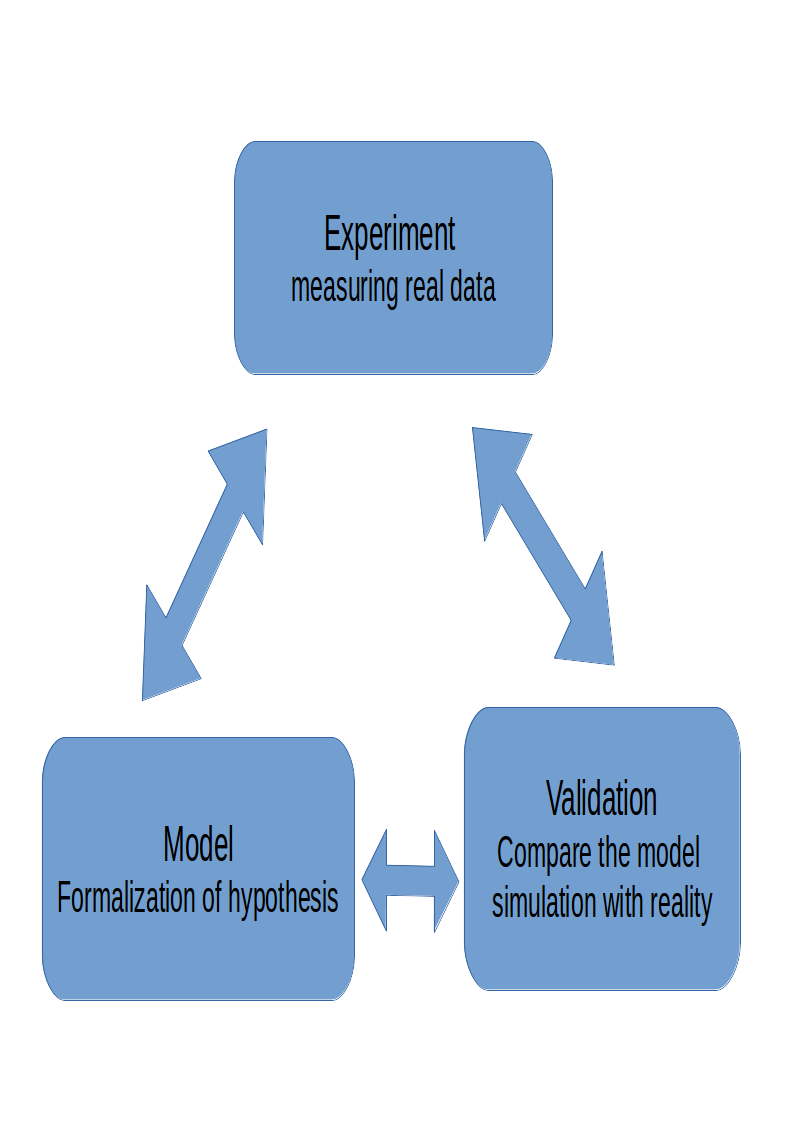
\includegraphics[width=0.5\textwidth, height=5cm]{chapter6/modeling.png}
    \caption{Schematic illustration of scientific process. The experiments produces data which are interpreted and hypothese is formalized as a model. Validation compares the model simulation with experiment, if model satisfies the criteria - is in agreement with real experiments, then the validated model can be used for other purposes.  %\bibentry{EGICompendium2013} \bibentry{egi2014}.
    }
    \label{fig:modeling}
\end{figure}

Application of the mathematical modelling techniques towards the biomedical research is sometimes called as systems biology approach combining the reductionism and integration as denoted by Kohl et al.\cite{Kohl2010}. Application towards the clinical praxis include the quantification of the diagnostic index or treatment strategy and it is a goal to develop tools, database models and methods of several Physiome projects, e.g. VPH-Physiome project presented by Hunter et al.\cite{Hunter2009}.

One of the earliest complex and integrative modelling effort was a model of circulation and it's regulation published by Guyton et al. in 1972 \cite{Guyton1972} which via derivative and technological upgrade continues as "Human Model" or "HumMod" introduced by Hester et al. \cite{Hester2011systems,hester2011} with a focus on integration effort. Different approach of modelling human physiology is a database of smaller models focusing on some particular physiological phenomenon. E.g. the NSR Physiome project introduces  JSIM\footnote{JSIM: \url{http://www.physiome.org/jsim/} accessed January 2015} Java based simulation system to support modeling in  physiology. Repository of several hundred of models were published using this system \cite{Butterworth2014}. The similar effort is done by IUPS Physiome project and repository of models are  based on XML standard languages CellML and FieldML \cite{Hunter2004,Yu2011}. The Systems Biology Markup Language (SBML) is used for modeling biological system at the level of biochemical reaction and regulatory network and another database collects several hundreds of curated and non-curated models \cite{Hucka2004,LeNovere2006}.

JSIM, CellML, SBML or HumMod are domain specific languages and the tools able to work with them are primarily developed within physiological or systems biological communities. Other authors use commercial or industry standard tools for mathematical modelling and computing. E.g. Kofranek et al. describes Guyton's 1972 model in MATLAB\textsuperscript{\textregistered} Simulink \cite{Kofranek2010} and the derivative HumMod in acausal object-oriented Modelica language \cite{Kofranek2011hummod,kofranek2013hummod}. Fernandez et al. describes models of cardiovascular pulsatile system using MATLAB Simscape  \cite{FernandezDeCanete2013} and recently in Modelica  \cite{FernandezdeCanete2014}.

Thus there is an open debate whether in-house domain specific language and tools like JSIM, CellML and FieldML,SBML or HumMod reached it's capabilities for representing complex models. Only the HumMod reached the integrative approach building the complex integrative model of human physiology using lumped parameter approach. I contributed to the idea of key features which involves acausal modeling technique and object orientation which keeps the complex model structure decomposed into understandable and maintainable parts and allows to cover complexity of models like HumMod. 

The methods and examples of modeling cardiovascular system are described in the next section \ref{sec:methodsmodels}. The methods of estimating parameters of complex models are described in section \ref{sec:methodsestimation} and particular results are described in section \ref{sec:resultsestimation}.

%\label{sec:results}
\section{Modeling methodology}
\label{sec:methodsmodels}
%For building complex models it seems that acausal (or declarative) modeling technique is key feature as it allows to express the variables declaratively, acausal modeling tool (e.g. Modelica or MATLAB\textsuperscript{\textregistered}  SIMSCAPE\texttrademark) figures out which are the dependent and independent variables upon compilation\cite{fritzson2002}. This allows building complex systems of equation from composed components and the model diagrams still captures the essence of the modeled reality much better and the simulation models are much more legible and thus also less prone to mistakes\cite{Kofranek2008,FernandezDeCanete2013}. 
The methodology of formalizing mathematical models is influenced by the abilities of underlying modeling language used. %As it was noted in previous chapter \ref{sec:intromodels}, the technology used for formalizing mathematically knowledge may introduce some benefits.
%\subsection{Modelica}
The Modelica language is an object-oriented, equation based and acausal modeling language standardized by Modelica association\footnote{\url{http://www.modelica.org} accessed February 2015}.

Object orientation means that the definition of model is class as in object oriented programming, instance of the model is object,  each instance can share type and differ in parameters and the place where it is used, inheritance and some sort of polymorphism is possible.

Equation based means that the equation is not statement, thus the relation among variables can be expressed in any form. Modelica tool will decide which one is input and output upon compilation. E.g. from the equation $q = \frac{dV}{dt}$ the process of computation can lead to $ q:= der(V)$ or $ V := \int{q}dt$ based on whether the $V$ or $q$ is known from the context.

Acausal connector is special purpose class to define variables of the model shared with other models or classes. Connecting two or more components via acausal connector will generate equality of all "non-flow" variables in connected connectors: $$p_1=p_2=\ldots =p_n$$
and zero sum of all "flow" variables $$ \sum_{i=1}^n q_i=0$$

%As an example, we will declare components important for modeling cardiovascular system (CVS). The components are hydraulic elastic ballon, which is analogy of electrical capacitor, and hydraulic resistor, analogy of electrical resistor.
%
%Connector \emph{HydraulicPort} with "flow" variable $q$ and non-flow variable pressure $p$ is presented in Modelica source code:
%\begin{lstlisting}[language=modelica]
%connector HydraulicPort
%  flow Real q;
%  Real p;
%end HydraulicPort;
%\end{lstlisting}
%
%Model of hydraulic resistor(conductor) with parameter $G$ denoting conductance and two hydraulic ports express the equations:
%\begin{equation}
%q_{in}.q = -q_{out}.q \label{eq:conductor1}
%\end{equation} 
%\begin{equation}
% q_{in}.q = G \times (q_{in}.p-q_{out}.p) \label{eq:conductor2}
%\end{equation}
%presented in Modelica source code:
%\begin{lstlisting}[language=modelica]
%model HydraulicConductor
%  parameter Real G;
%  HydraulicPort qin;
%  HydraulicPort qout;
%equation 
%  qin.q= -qout.q;
%  qin.q = G*(qin.p-qout.p);
%end HydraulicConductor;
%\end{lstlisting}
%
%
%Model of hydraulic elastance with parameters $V_0$ as unstressed volume $p_0$ external pressure and $C$ compliance(reciprocal value of elastance) with state variable $V$ volume express these equation:
%\begin{equation} \label{eq:compliance}p-p_0 = \left\{   
%  \begin{array}{l l} 0 & \quad \text{if } V \text{\textless} V_0 \\ 
%    \frac{V-V_0}{C} & \quad \text{otherwise}
%  \end{array} \right.\end{equation} 
%\begin{equation}\label{eq:flowrate}\frac{{\rm d}V}{{\rm d}t} =  q\end{equation} 
%is presented in Modelica source code:
%\begin{lstlisting}[language=modelica]
%model HydraulicElastance
%    Real V;
%    parameter Real V0;
%    parameter Real p0;
%    parameter Real C;
%  HydraulicPort qin;
%equation 
%   qin.p -p0 = if (V<V0) then 0 else (V-V0)/C;
%   der(V) = qin.q;
%end HydraulicElastance;\end{lstlisting}

The paper \cite{Kulhanek2014Modeling} \emph{Modelling of Short-term Mechanism of arterial pressure in the cardiovascular system: Object-oriented and acausal approach} in Appendix~\ref{app:d} published disputation about causal and acausal approach in using Modelica for modeling lumped parameter CVS model. 

The paper \cite{Kulhanek2014mefanet} \emph{Simple Models of the Cardiovascular System for Educational and Research Purposes} in Appendix~\ref{app:simplemodelsd} published detailed methodology of modeling pulsatile CVS in Modelica. 

Comprehensive guide to the Modelica language and it's capabilities are in the book of Fritzson \cite{fritzson2002} or in the on-line book by M.Tiller \cite{Tiller2014}.

\section{Parameter Estimation}
\label{sec:estimation}

%\subsection{Identification of physiological systems}
%Model verification (whether simulation of the model shows desired behavior) and model validation (whether model simulation agrees with new observation of real system) are important steps in system analysis and model construction. 
Usually some knowledge of the system - the structure is available and unknown coefficients (parameters) remain unknown. Once the model is formalized and constructed, further problem is to estimate the model parameters so that the model reproduces real world system. This procedure is sometimes called model identification \cite[p.~159]{khoo2000}. The objective of this task is usually to minimize the following function (to find least squares of the differences between predicted and measured values):
\begin{equation} \label{eq:parameter} 
f( \vec{p} ) = \sum_{i=1}^{n} ( M(t_{i},\vec{p} ) - d(t_{i}) )^2 \to min  
\end{equation} 
where $\vec{p}$ is vector of values of parameters, $M(t_{i},\vec{p})$ is model simulated at time $t_{i} $ with the given parameter values $\vec{p}$ and $d(t_{i})$ is the measured experimental value at time $t_{i}$.
Algorithmically, this problem was shown to belonging to the \emph{NP-complete} problems \cite{Hofmann2005} thus the best exact algorithm is based on brute force search - trying all possible values of parameters and simulate the model with them and find minimum of the objective function \ref{eq:parameter}. 
However, exact solution may not be needed because the models itself are by definition approximation of real system, and the input data are measured with some degree of error. 
As in other problems where exact algorithm uses brute-force search, some heuristic or randomization method should be used for bigger space of potential input data. 
After the parameter estimation a further problems arise with structural identifiability and analysis of sensitivity to the estimated parameter values\cite[p.~176]{khoo2000}. 

Parameter estimation and further analysis methods are part of specialized mathematical software. E.g. Pruet et al. used Metropolis algorithm to produce a distribution of parameters to calibrate the model of human cardiovascular physiology, which were further tested against predictive ability of circulatory failure and statistical methods performed in the software Wolfram \textit{Mathematica} \cite{Pruett2013}. The iterative improvement method in the software MATLAB Simulink\textregistered ~was used in estimating 2 parameters of simple cardiovascular model by Takahashi et al. \cite{Takahashi2013}. Several methods were compared in estimating multiple parameters of cardiovascular system in MATLAB Simulink\textregistered ~by Abbass et al. \cite{Abbass2012}.

Heuristic methods reduce the number of simulation and additionally some set of  simulation can be computed concurently e.g. in grid or cloud computing infrastructure. 
Maffioletti et al. published GC3Pie framework utilizing evolutionary algorithms and introduced workflow to identify parameters of models for economical predictions using grid computing \cite{maffioletti2012computational}. Humphrey et al. calibrated hydrology models utilizing commercial Windows Azure cloud computing infrastructure with a significant speedup on the modified dynamically dimensioned search algorithm\cite{Humphrey2012,Tolson2007}. 

%Selected methods to estimate parameters are introduced in section \ref{sec:methodsmodels}. 

As already identified also by other authors of some calibrating systems, the parameter estimation is used sporadically, however, with high demand of computational task in temporal time. Thus, I proposed and designed the system which can distribute the simulation task into grid-computing and cloud-computing infrastructure and the computational capacity can be provisioned on-demand.% this brings significant speedup for parameter estimation of complex model but limited speedup on simple models. 
Methods are described in section \ref{sec:methodsestimation} and interesting results are described in section \ref{sec:resultsestimation}.

\section{Methods for Parameter Estimation}
\label{sec:methodsestimation}
Evolutionary algorithms are used for finding global minimum or maximum and it can be used to estimate the parameters of the model. Genetic algorithm is type of evolutionary algorithm and the general structure of the algorithm is presented in figure \ref{fig:GA-kopenogram}.

\begin{figure}[htb]
    \centering
    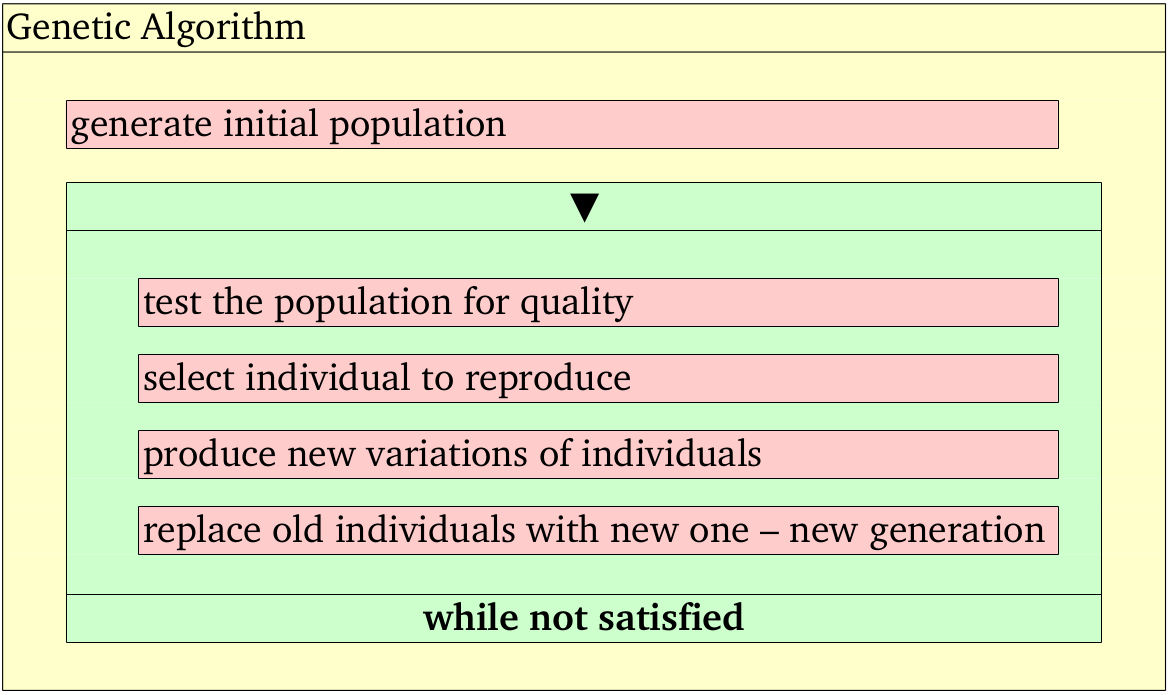
\includegraphics[width=0.6\textwidth]{chapter6/GA-kopenogram.png}
    \caption{General structure of genetic algorithm presented as kopenogram. Kopenograms are graphical language for structured algorithms to supplement UML proposed by Kofranek et al.\cite{Kofranek2012}.
    }
    \label{fig:GA-kopenogram}
\end{figure}


\begin{figure}[htb]
    \centering
    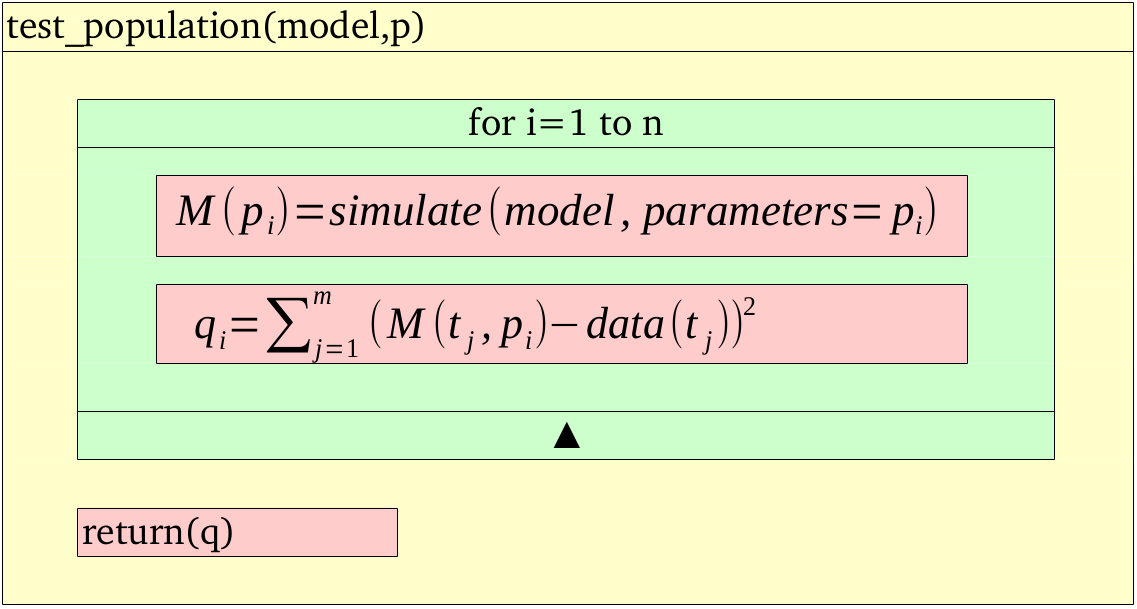
\includegraphics[width=0.6\textwidth]{chapter6/GA-kopenogram2.png}
    \caption{Specific test of the population for quality in case of parameter estimation. Model is simulated according to individual $i$ with parameters $p_i$ and the quality $q_i$ is counted per the objective function \ref{eq:parameter}.
    }
    \label{fig:GA-kopenogram2}
\end{figure}

The iteration within the loop "$\blacktriangledown \ldots$ \emph{while not satisfied}" depends on previous iteration, thus in general it cannot be parallelized.
In the case of parameter estimation, the step \emph{test the population for quality} has algorithmical structure as in fig.\ref{fig:GA-kopenogram2}. Each iteration in the loop "\emph{for i=1 to n}" is independent and a therefore loop parallelism (section \ref{sec:parallelprogramming}) can be utilized and implemented here.

The Amdahl's law in equation \ref{eq:amdahl} can be used to estimate  the theoretical speedup limitation for the specific model and potential gain for identifying different types of models can be stated. We assume that the simulation of the model with any parameters will take the same time, even this is not generally true as the non-linear models and numerical methods may cause different steps to be performed for different parameter values. 

The specific fraction $\alpha$ for the model determines the level of scalability of the model within the parallelized system. For the complex models the $\alpha$ will decrease. The specific estimates of the fraction $\alpha$ and it's influence on the scalability and results are presented in section \ref{sec:resultsestimation}.

\subsection{Architecture of system for parameter estimation}

The architecture of the system implementing the algorithms in fig. \ref{fig:GA-kopenogram} and \ref{fig:GA-kopenogram2} will determine the overhead which may affect significantly the computation time.

The architecture of the proposed system is in fig \ref{fig:architectureestimation}.
\begin{figure}[htb]
    \centering
    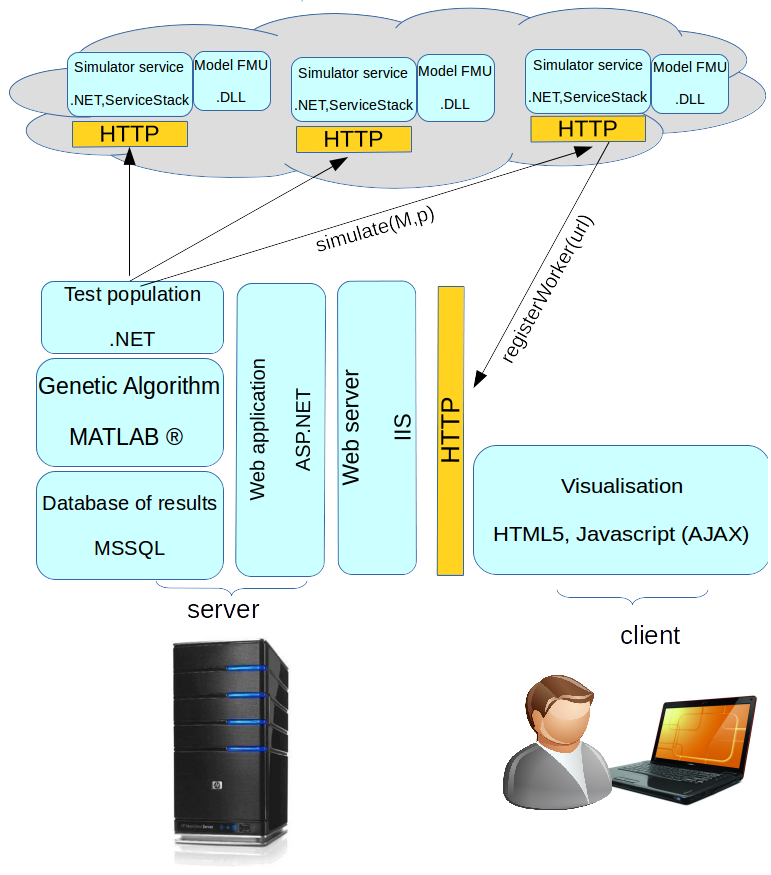
\includegraphics[width=0.6\textwidth]{chapter6/architekturaestimation.png}
    \caption{Architecture of the system employing genetic algorithm and concurent simulation of models in cloud.
    }
    \label{fig:architectureestimation}
\end{figure}
Modelica models can be exported as proprietary C/C++ code or binary EXE with some default command-line options to perform simulation. Modelica models can be exported into standard Functional Mockup Unit(FMU) with is standardized XML metadata packaged together with  binary library .DLL (or .SO) following standardized API\footnote{\url{https://www.fmi-standard.org/} accessed February 2015}.


\section{Results}
\label{sec:resultsestimation}

The paper \cite{Kulhanek2014Parameters} \emph{Parameter estimation of complex mathematical models of human physiology using remote simulation distributed in scientific cloud} in Appendix~\ref{app:c} published the architecture and results achieved on estimating parameters on three  different types of models from the non-complex, medium-complex and complex model.

\chapter{Results}
\label{sec:results}
In previous chapters, different methods were introduced that are available for selected use cases in biology and medicine research. 
%\section{Virtual Infrastructure}
%\label{sec:resultsinfrastructure}
As each of the use cases and available systems were proposed on different operating system platforms, architecture and/or middleware, the virtualization was utilized to build the virtual infrastructure for the purposes of each pilot application. The paper \cite{kulhanek2010c} \emph{Infrastructure for Data Storage and Computation in Biomedical Research} in Appendix~\ref{app:infrastructure} describes the result of establishing virtualization on a physical infrastructure in order to share computational power among different platforms.

\section{Medical Images}
\label{sec:resultsimages}

%Within the virtual infrastructure, the pilot grid infrastructure was established in the location of First Faculty of Medicine, Charles University in Prague, Central Military Hospital in Prague and CESNET association. And the Globus Toolkit middleware and Globus MEDICUS implementation was installed on linux based virtual machines using XEN hypervisor providing pilot services to access this grid based PACS system.

The pilot infrastructure of several servers was installed in several institutions in Prague, Czech Republic. Globus Toolkit and Globus MEDICUS were installed on them. The paper \cite{kulhanek2009}  \emph{Processing of Medical Images in Virtual Distributed Environment}, in Appendix~\ref{app:processing}, published details about the integration of Globus MEDICUS with a MeDiMed project. It concludes that such integration via the DICOM protocol is almost seamless. Furthermore, if such a grid-based system is joined with a production system for exchanging clinical DICOM data, it could be beneficial for researchers.

\section{Remote Access To Voice Analysis}
\label{sec:resultsvoice}

The paper \cite{kulhanek2010b} \emph{Remote Analysis of Human Voice--Lossless Sound Recording Redirection}, in the Appendix~\ref{app:remote}, published technical details and results of customizing a RDP protocol for lossless sound recording redirection. It also discusses remote access via a remote desktop feature of Windows platform to an application in order to analyze human voice and produce a voice range profile for further use. 

Additionally, the 
%custom RDP plugin with the ParVRP and RealVoiceLab software to redirect the sound recording without loss of information 
remote application
was packaged as a virtual machine template. This was deployed in the pilot virtual infrastructure next to the test instance of Globus MEDICUS. The virtual machine template was also deployed to different cloud computing infrastructures. The first was deployed to the Amazon EC2\footnote{\url{http://aws.amazon.com/ec2/} accessed February 2015} and the second to the pilot scientific cloud, MetaCloud\footnote{\url{http://www.metacentrum.cz/en/cloud/} accessed February 2015}. In the EGI Technical Forum 2012, such comparison was presented to the user and technical community within CESNET and EGI organization\cite{Kulhanek2012a}.

\section{Parameter Estimation}
\label{sec:resultsestimation}

The paper \cite{Kulhanek2014Parameters} \emph{Parameter Estimation of Complex Mathematical Models of Human Physiology Using Remote Simulation Distributed in Scientific Cloud}, in Appendix~\ref{app:parameter}, published the architecture and measurement of a speedup that was achieved on estimating parameters of three different types of models - from the non-complex, medium-complex and complex models. It concluded that only medium-complex and complex models may benefit from the architecture as the communication overhead may become major for simple models and decrease the overall performance. 

Additionally, a scientific result was published in the paper \cite{Matejak2014sj} \emph{Adair-based Hemoglobin Equilibrium with Oxygen, Carbon Dioxide and Hydrogen Ion Activity}, in Appendix~\ref{app:adair}, where a mathematical model of hemoglobin integrating \ce{O_2}, \ce{CO_2} and \ce{H^+} binding based on theoretical principles, which were verified on the parameter estimation algorithm system\cite{Kulhanek2014Parameters}, together with methods available in Wolfram \emph{MATHEMATICA} 9.0\footnote{\url{http://www.wolfram.com/mathematica/}accessed February 2015}.

Thus, the overall performance and speedup estimation were tested against the Modelica implementation of complex physiological model HumMod \cite{Kofranek2011hummod}; the Modelica implementation of a model of hemodynamics of the cardiovascular system, published by Meurs \cite{Meurs2011}; the model of binding gases to hemoglobin, published by Matejak \cite{Matejak2014sj} and the trivial model of a curve $f(x)$ with four parameters $a,b,c,d$ defined as $ f(x)=a\cdot sin(b\cdot (x-c))+x\cdot d$ and named as "SinusCurve".
%corrections April 2nd
\sisetup{round-mode=figures,round-precision = 4}
\begin{table}[htb]
\footnotesize
\begin{tabular}{|l|r|r|r|r|r|r|r|}
\hline
complexity & name & $T_{1~[s]}$ & $T_{2~[s]}$ & $T_{3~[s]}$ & $T_{4~[s]}$ & $\alpha$ & $S$ \\
\hline
high & HumMod \cite{Kofranek2011hummod} & $\num{4639}$ & $\num{4639}$ & $\num{4618}$ & $\num{4616}$ & $\num{8.85837717978788E-005}$ & $\num{11288.7493917249}$ \\
medium & Meurs2011\cite{Meurs2011} & $\num{661.817}$ & $\num{661.490}$ & $\num{634.694}$ & $\num{634.457}$ & $\num{0.0004940943}$ & $\num{2023.9051987766}$ \\
low & Matejak2014\cite{Matejak2014sj} & $\num{17.868}$ & $\num{17.610}$ & $\num{1.399}$ & $\num{1.123}$ & $\num{0.014439221}$ & $\num{69.2558139535}$ \\
trivial & SinusCurve & $0.073$ & $0.020$ & x & x &  $\num{0.7260273973}$ & $\num{1.3773584906}$\\
\hline
\end{tabular}
\caption{Time spent in different parts of the parameter estimation algorithm for one processor deployment utilizing virtual machine on physical hardware 2x 6-core Intel E5-2620 2GHz. Genetic algorithm works with a population of $120$ individuals for $10$ generations. T1 -- is the whole time of the computation, T2 -- is the time of the computation, which can be parallelized, T3 -- time spent within the worker node, T4 -- time spent in simulation, $\alpha$ -- computed as $1-(T2/T1)$ and $S$ is the theoretical speedup limit per Amdahl's law ($1/\alpha$) eq.(\ref{eq:amdahl}).}
\label{table:speedupresult}
\end{table}

\begin{table}[htb]
\footnotesize
\begin{tabular}{|l|r|r|r|r|r|r|r|}
\hline
complexity & name & $T_{1~[s]}$ & $T_{2~[s]}$ & $T_{3~[s]}$ & $T_{4~[s]}$ & $\alpha$ & $S$ \\
\hline
high & HumMod \cite{Kofranek2011hummod} & $\num{6463.217}$ & $\num{6460.937}$ & $\num{6451.079}$ & $\num{6458.253}$ & $\num{0.000352766}$ & $\num{2834.744}$ \\
medium & Meurs2011\cite{Meurs2011} & $\num{699.631}$ & $\num{699.228}$ & $\num{697.907}$ & $\num{696.948}$ & $\num{0.000576018}$ & $\num{1736.057072}$ \\
low & Matejak2014\cite{Matejak2014sj} & $\num{2.893}$ & $\num{2.373}$ & $\num{1.228}$ & $\num{1.149}$ & $\num{0.17974421}$ & $\num{5.563461538}$\\ \hline
\end{tabular}
\caption{Same as Table \ref{table:speedupresult}, but measured on a local server deployment, with reduced communication overhead.}
\label{table:speedupresult2}
\end{table}

The computation time of a single simulation depends mainly on the model complexity. Based on the findings, the simulations of the models were divided into four groups, depending on its demand to compute $\num{1200}$ simulations. Speedup is studied for these four groups and Amdahl's law is appropriate to estimate upper limit of it as discussed in Section \ref{sec:parallelprogramming}. Fraction $\alpha$ and the speedup limit per Amdahl's law are stated in Tables \ref{table:speedupresult} and \ref{table:speedupresult2}. 

The difference between $T_2$ and $T_3$ is an overhead, which was introduced by the network communication between the genetic algorithm and the worker nodes that were deployed in the cloud deployment, provided by CESNET NGI department METACENTRUM\footnote{\url{http://www.metacentrum.cz} accessed March 2015}. The network overhead can be eliminated in serial implementations by directly integrating the simulation into a genetic algorithm. Therefore, Table \ref{table:overhead} considers and compares a hypothetical serial execution time, which is estimated without the network overhead.

\begin{table}[ht]
\footnotesize
\begin{tabular}{|l|r|r|r|r|r|r|r|r|}
\hline
& \multicolumn{4}{c|}{distributed in cloud} & \multicolumn{4}{c|}{distributed in local cluster} \\
 & \multicolumn{2}{c|}{overhead} & \multicolumn{2}{c|}{est. serial} & \multicolumn{2}{c|}{overhead} & \multicolumn{2}{c|}{est. serial} \\
model name & $T_2-T_{3~[s]}$ & fraction$_{[\%]}$ & $T_{es~[s]}$ & $S_{es}$ & $T_2-T_{3~[s]}$ & fraction$_{[\%]}$ & $T_{es~[s]}$ & $S_{es}$\\
\hline
HumMod \cite{Kofranek2011hummod} & $\num{20.983}$ & $\num{0.45225141}$ & $\num{4618.693}$ & $\num{1.0045430601}$ & $\num{9.858}$ & $\num{0.15252466}$ & $\num{6453.359}$ & $\num{1.0015275766}$ \\
Meurs2011 \cite{Meurs2011} & $\num{26.796}$ & $\num{4.04885338}$ & $\num{635.021}$ & $\num{1.0421970297}$ & $\num{1.321}$ &  $\num{0.18881382}$ & $\num{698.310}$ &$\num{1.00189171}$\\
Matejak2014\cite{Matejak2014sj} & $\num{16.211}$ & $\num{90.72643833}$ & $\num{1.657}$ & $\num{10.7833433917}$ & $\num{1.145}$ &  $\num{39.57829243}$ & $\num{1.748}$ &$\num{1.6550343249}$\\
\hline
\end{tabular}
\caption{ Comparison in cloud deployment vs. local cluster deployment of communication overhead. Its fraction in the whole computation was introduced by the network transfer speed and latency. The estimated time and speedup, if the worker is replaced by a serial version of computation without communication overhead, is: $T_{es}$ -- estimated time of serial version of computation. $S_{es}$ -- estimated speedup of serial version of computation against the parallel on one processor.}
\label{table:overhead}
\end{table}

The speedup was measured on 10 CPUs till 60 CPUs and compared in order to predicted the speedup, as seen in Figure \ref{fig:amdahlres}. Similar  measurements with different parameters of genetic algorithm were carried out using 80 and 160 CPUs, as seen in Table \ref{table:speedupresult3}.

\begin{table}[htb]
\footnotesize
\begin{tabular}{|l|r|r|r|}
\hline
complexity & name & S(80) & S(160)\\
\hline
high & HumMod \cite{Kofranek2011hummod} & $\num{63.9807249802}$ & $\num{121.5389821285}$ \\
medium & Meurs2011\cite{Meurs2011} & $\num{55.9311360464}$ & $\num{53.0128125}$ \\
low & Matejak2014\cite{Matejak2014sj} & $\num{16.6865881526}$ & $\num{12.5500720509}$\\ \hline
\end{tabular}
\caption{Scalability on 80 CPUs and 160 CPUs of parameter estimation on cloud computing cluster on 5-10 virtual machines, each 16 CPUs on physical hardware 2x 8-core Intel E5-2670 2.6GHz. Genetic algorithm configured with a population $640$ individuals for $20$ generations, which increases about 10 times more simulation performed compared to previous tables. Speedup estimated from measuring the computation when using 1 CPU.}
\label{table:speedupresult3}
\end{table}

\begin{figure}[htb]
    \centering
    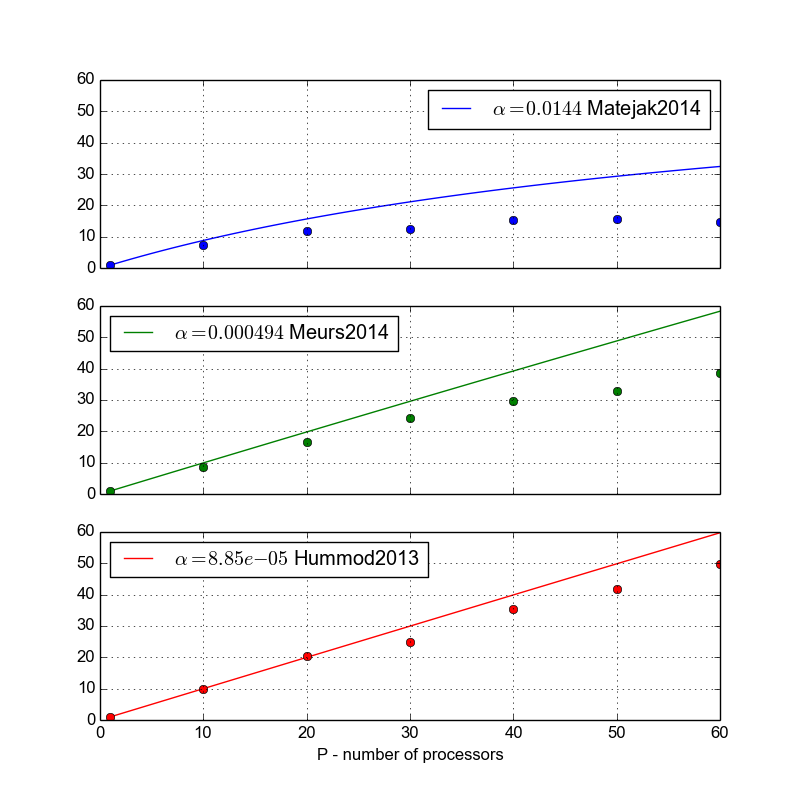
\includegraphics[width=0.9\textwidth]{chapter7/speedup.png}
    \caption{Estimated speedup (lines) per Amdahl's law (eq.\ref{eq:amdahl} \cite{Amdahl1967}) for different $\alpha$ of several Modelica models and real measured speedup (points) on cloud deployed on 1-6 virtual machines on physical hardware (2x 6-core Intel E5-2620 2GHz, 1Gbit/s Ethernet.)  }
    \label{fig:amdahlres}
\end{figure}

To summarize the results, the simple models scale up to the 20 processors with speedup of 15. The medium scales up to 80 processors with a speedup of about 56 and complex models scale up to 160 processors with a speedup near 120. Practically, after 200 generations, a good approximation was obtained, which implicates that the computation time could be reduced from four days to 47 minutes in the case of HumMod and from 17 hours to 18 minutes, in the case of the medium complex model.

The deployment on local cluster reduces the communication overhead. However, in order to compute concurrently, it is limited by available processors. Thus, computing on local cluster should be considered for boundary cases like the simple models. The following statement can be made:
\begin{itemize}
\item{If the alpha fraction is major, then a serial computation of parameter estimation algorithm without communication overhead, will perform best. This is the case for the trivial function. }
\item{If the alpha fraction is minor, but the network overhead is still major a computation on local cluster or virtual HPC cluster should be considered. This is the case for the low complex model simulation, e.g.  Matejak2014\cite{Matejak2014sj}.} 
\item{If the alpha fraction is minor and the network overhead is also minor, then the distributed computation, e.g., in a cloud-computing environment, is worth using. This is the case of the medium and high complex model simulations of "Meurs2011" \cite{Meurs2011} and "HumMod2013" \cite{Kofranek2011hummod}.}
\end{itemize}

\begin{figure}[htb]
    \centering
    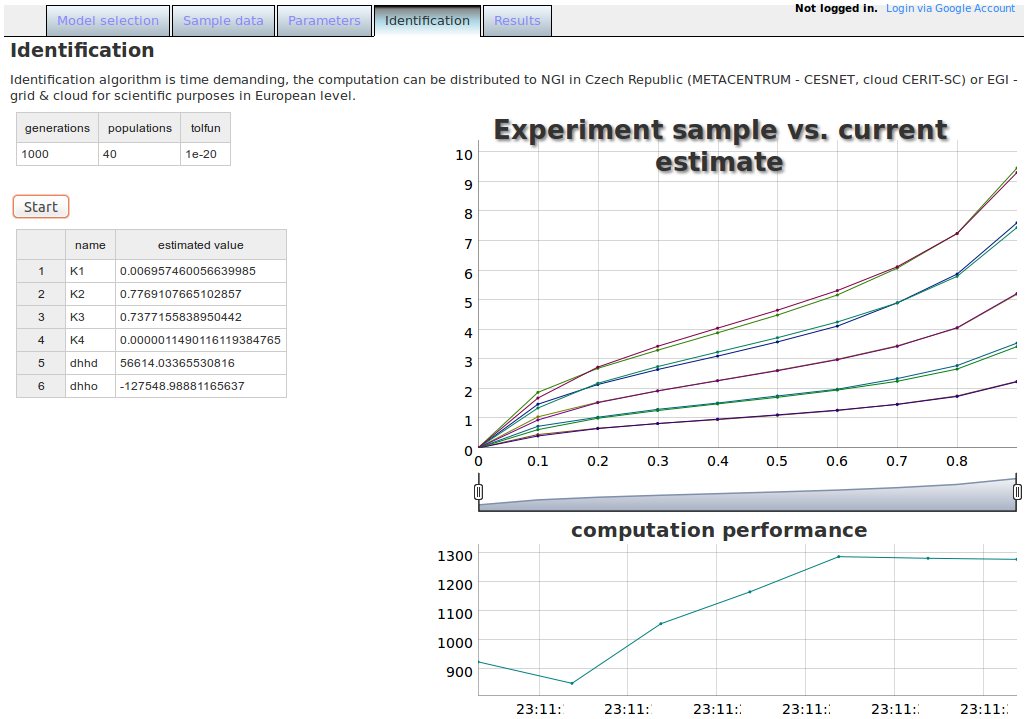
\includegraphics[width=1\textwidth]{chapter7/app-physiovalues.png}
    \caption{User interface of a web application for parameter estimation. In this case, for the model Matejak2014\cite{Matejak2014sj}. The top left table lists the parameters for the genetic algorithm($\num{1000}$ generations with a population size of $40$ and a cumulative change in the generation limit, which ends the algorithm earlier). The middle left table shows the model parameters and current best values, which fit the sample data. The chart shows how the sample data fits with the model simulation. The right bottom chart shows the performance of computation in a number of model simulations per second.}
    \label{fig:app.physiovalues}
\end{figure}

\subsection{Parameter Sweep}
\label{sec:resultsboinc}
The desktop grid BOINC system was established for parameter sweep application. The established project, \emph{Physiome@home}, and it's project web page, \url{http://physiome.lf1.cuni.cz/ident3/physiome}, manages workunit tasks which are sent to and executed by BOINC workers. The worker application is a packaged model that is exported as FMU for a Windows platform and wrapper application, which communicates with the BOINC manager on the desired volunteer computer. 

%This project is now  distribute computational tasks into computers in scholar labs, which may in iddle time contribute to the computing demands. Because BOINC is very popular and users joins to a teams to compete with several types of competition, this particular project attracts after 2 weeks 78 participants from all around the world. 


\subsection{Remote Simulation and Local Visualization}
An extra outcome of an architecture for parameter estimation is a hybrid web simulator system, where a single instance of a worker node is utilized as a back-end for the simulation engine. The front-end presented as a web application, is implemented using HTML and Javascript libraries in order to visualizes and control the simulation on the worker, as seen in Figure \ref{fig:sim.physiovalues}.
The results were published in \cite{Kulhanek2013c} and popularized in \cite{Kulhanek2013b}.

\begin{figure}[htb]
    \centering
    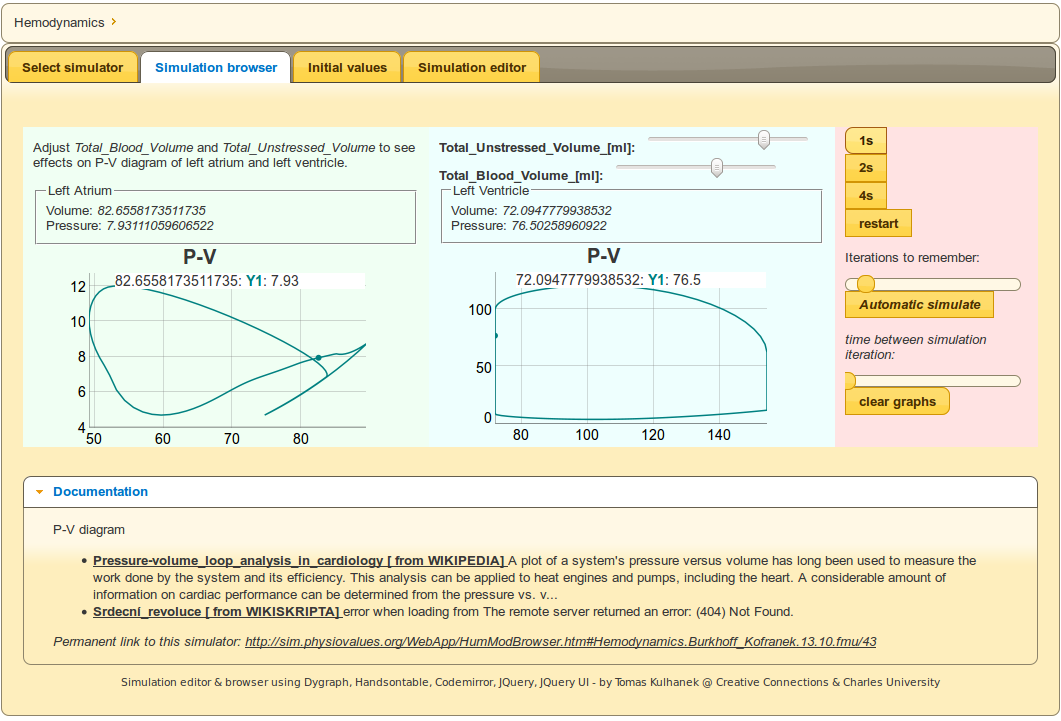
\includegraphics[width=1\textwidth]{chapter7/sim-physiovalues.png}
    \caption{Web application to visualize simulation, in this case, pressure volume diagrams of the left atrium and left ventricle of the model of hemodynamics of a cardiovascular system.}
    \label{fig:sim.physiovalues}
\end{figure}

\subsection{Summary}

A pilot web domain was established to include the previous results and to start collecting the physiological relevant values at \url{http://www.physiovalues.org}. 
Further development may focus on connecting values of parameters and variables with a physiological or pathological scenario. 
\chapter{Conclusion}
\label{sec:conclusion}

\section{Discussion}
\label{sec:discussion}
%Important decision about utilizing distributed computing infrastructure is what benefits it'll bring with respect of the caveats and resources it'll consume including the human capital compared to other existing solution.

%\subsection{Medical imaging}
%There are several use cases where exchanging or sharing DICOM images are beneficial, next to the second opinion and teleradiology (remote diagnostics), gathering information and expertize in rare diseases, studies in unusual cases or secondary use of clinical imaging data for research, optimizing new processing methods etc. 

%The Globus MEDICUS stores one or more copies of DICOM images within grid infrastructure, and as such, can be used as technology and infrastructure to built data warehouse for DICOM images of specific interest. Another philosophy is to federate files and metadata stored within home institutions, which seems to be preferred solution in hospitals and clinical use which were shown in other medical sharing image projects.

The result presented in section \ref{sec:resultsimages} is an example how a standard format and protocol DICOM is utilized to integrate current production system in order to exchange medical images (MEDIMED \cite{Slavicek2010}) and a grid-based solution (Globus MEDICUS\cite{Erberich2007}). Remote Desktop Protocol (RDP) is a key standard for protocol in order to integrate the application of voice analysis\cite{Fric2007} into a remote environment, which is accessible via the Internet. This is presented in section \ref{sec:resultsvoice}. In the case of parameter estimation, a key factor is the standard Functional Mockup Interface (FMU)\cite{Blochwitza},  which allows the control and simulation of a physiological model in a customized tool that is not related to modeling tool. This is presented in section \ref{sec:resultsestimation}. 

The selection of a joint element increases the chances of reusability of such a system in future development, when requirements usually change and the reconstruction of a system or architecture is needed. For example, the presented solution, which is based on Globus MEDICUS, is, in general, a data warehouse, that stores one or more copies of DICOM images. However, federated files and metadata that are stored within home institutions, which only share network infrastructure to interchange the DICOM studies, seems to be a preferred and more acceptable solution by hospitals. Thus, in their further development, the authors of Globus MEDICUS followed a way of federation of medical images that are stored within home institutions, as published by Chervenak et al. \cite{Chervenak2012}. The grid computing infrastructure seems to be suitable for research and educational purposes, but not generally acceptable for clinical use. %Cloud-computing with ability of hybrid cloud, where part of virtual machines may reside in home institution may be also answer on this issue.

%here an underlying technology is hidden for common user. This research was originally motivated by the idea to investigate benefits and show robust grid-based technology against proprietary distributed technology, which may face up to scalability and maintenance issues. Another issue is the philosophy of storing medical images. The presented solution based on the Globus MEDICUS is in general a data warehouse storing one or more copies of DICOM images, in contrast to federated files and metadata stored within home institutions which shares only network infrastructure to interchange the DICOM studies. This seems to be more acceptable by hospitals and by the national and international regulation for clinical and diagnostic use, e.g. The authors of Globus MEDICUS in their further development followed a way of federation of medical images stored within home institutions rather than in a grid infrastructure published by Chervenak et al. \cite{Chervenak2012}. 
%

%However, the scalability is managed within the current MEDIMED system and separate PACS system including database of anonymized medical images with the medical context and description for research and education purposes coexist within the current system.


%This allows to keep current tools for processing the medical images when the technology of infrastructure is changed.
%Thus user experience is kept on using same tools or same workflows, however, accessing much broader database of records or having more powerful tools for processing the data.
 
In the case of remote voice analysis, the remote access to an legacy application via network protocol keeps the majority of user experience, as presented in section \ref{sec:resultsvoice}. Such service can be deployed on any web server and the occasional need to educate or perform a higher number of analysis concurrently can be satisfied with cloud computing deployment. The application process for sound signal which is currently analyzed by Fast Fourier Transformation algorithm quite effectively. Another challenge is to analyze a sound signal connected with high-speed video or videokymography methods. This need however to transfer, process and store large amounts of data (GB). With current common network speed available in departments of laryngology (up to one GBit) this may introduce impractical latency needed to transfer data to remote application and is not suitable for real-time analysis compared to analysis of sound signal. But for post-processing and storing such records, this system can bring benefits for second study, gradual improvement of diagnostic methods, etc.  
%added 25th March
%Gaining access to advanced services to support clinical or therapeutist decision becomes more widely adopted by companies utilizing cloud-computing with heavy encryption mechanism, at the same time the database of anonymized records from history gradually improve algorithms for further diagnostics. E.g. Fetview\footnote{\url{http://fetview.com/} accessed March 2015} is an startup company to support such use cases in fetal healthcare.
%Such future application might utilize the results of grid-based systems for sharing medical images.

In the case of the application for parameter estimation presented in section \ref{sec:resultsestimation}, the computation is sensitive on communication overhead. For simple models, local high performance computing (HPC) resources are most beneficial. For medium and highly complex models, the deployment of worker nodes into a cloud computing environment is worth considering. Another challenge is an optimal size of population for genetic algorithm so the algorithm will converge to some acceptable solution in a reasonable time, as Gotshall et al. proposed a method for determining the optimum population size for a given problem \cite{Gotshall2000}.

%added 25th March, compare with existing publication 
The parameter sweep problem is considered as embarrasingly parallel and highly suitable for high throughput computing (HTC), which is the main focus of current grid computing infrastructures. Tøndel et al. introduced methods to statistically map variation of large number of parameters and to reduce drastically the number of simulations required for  parameter study \cite{Tondel2011}, however only non-complex models focusing on specific phenomenon were considered.

%Magnetic Particle Imager \footnote{introduced first by Gleich and Weizenecker\cite{Gleich2005}} (available only for animal models and not yet for human medicine) can produce high resolution images with fast shutter speed (~20 ms). Several computational and storage demanding biomedical application were shown in animal models by Saritas et al.\cite{Saritas2013}. There are research infrastructures which were established to coordinate the research in biology and medicine, e.g. Integrated Structural Biology Infrastructure for Europe (INSTRUCT)\footnote{\url{https://www.structuralbiology.eu/} accessed March 2015}, European Life Science Infrastructure for Biological Information (ELIXIR)\footnote{\url{http://www.elixir-europe.org/} accessed March 2015},  European Biomedical Imaging Infrastructure (Euro-BioImaging)\footnote{\url{http://www.eurobioimaging.eu/} accessed March 2015} and others. The purpose of these initiatives is to understand high-level phenotypes from genomic, metabolomic, proteomic, imaging and other types of data and they requires also multiscale mathematical models and simulation. As noted by Hunter et al.\cite{Hunter2013} such mathematical models can be delivered by physiome projects e.g. by virtual physiological human (VPH)\footnote{\url{http://www.vph-institute.org/} accessed March 2015}. 
%The medical imaging and processing methods are used to identify the parameters of models of human physiology for further diagnosis statement and treatment decision. Current studies focus on very simplified models and reduced number of parameters, e.g. Ralovich et al.\cite{Ralovich2012}
  
%The added value of the grid-computing or cloud-computing technology is the ability of enhanced collaboration in use cases which were difficult to achieve, e.g. in cases if secondary use of clinical imaging data for research

%for is an important area in research of rare diseases. As seen from the results obtained either in previous chapter or by other authors, the grid-computing is only one technology to facilitate some interconection of storage and computation capacity of different sites and servers owned by different organizations or individuals. 

%As seen from the results, there are several main purpose for which the grid-computing or cloud-computing infrastructure was built and are currently used for:
%\begin{enumerate}
%\item{solve big computational problems in distributed environment and achieve results in a reasonable computational time}
%\item{facilitate processing of the computation to support processing, analysis for further scientific results. This is provided by scientific portals, services, workflows etc. which allows non-exports in grid-computing or cloud-computing to do their job reducing researcher's time.}
%\item{share and archive database of scientific data for further processing and reproducibility.}
%\end{enumerate}
%\subsubsection{Scalability}
%
%From the perspective of efficiency (time complexity) and scalability (degree of parallelization) the heuristic methods for parameter estimation application brings at least some solution in a reasonable time. For small models it, however, doesn't make sense as the overhead and parallelizable fraction limits the speedup gain from distribution to grid or cloud-computing\ref{sec:resultsestimation}. 
%
%For complex models the infrastructure of grid-computing or cloud-computing can be used to distribute simulation tasks to explore wider space of possible solution.

%\subsubsection{Platform}

When porting an application to a grid environment, one of the important decision to consider is the platform of the used system. The architecture, which involves computational nodes that are deployed in a cloud computing infrastructure is influenced by the fact that the model implementation is exported from a third party tool to the standard FMU library for the MS Windows platform, as mentioned in section \ref{sec:methodsestimation}. This determines the platform of the worker node and the virtualization - or, in the case of parameter estimation, cloud computing is utilized on a prepared platform with a MS Windows license. In the case of parameter sweep, a desktop grid computing BOINC worker and application for a MS Windows platform is only prepared for volunteers with the compatible system. To utilize the service grid infrastructure, an export of the model into a FMU library and implementation of the wrapper service must be done in the grid computing platform,  which is usually a Linux based system. Another option is to use WINE\footnote{\url{https://www.winehq.org/} WINE. Accessed March 2015} -- a compatibility layer that is capable of running Windows applications on several POSIX-compliant operating systems, such as Linux, Mac OSX and BSD. 

%With respect to scalability the degree and fraction of paralelization from the whole computational process needs to be considered, as, e.g. for simulating simple models and estimating the parameters takes couple of minutes to hours on single computer, which may be acceptable and deployment on grid computing will introduce overhead which degrades the benefits.

%\subsubsection{Porting}
%Each of the introduced systems and application was from it's beginning prepared for serial workflow. To achieve higher level of programming model,  some manual intervention is usually needed on the system or source code of application.

For smaller types of application and scientific community with their own tools, the question is, whether or not to invest on porting their tools to grid specific platform and parallel programming model. 
In the case of integrating with a service grid middleware or with desktop grid framework, expert knowledge is needed to configure and customize the system. This is the case for the sharing of medical images (section \ref{sec:resultsimages}) and for parameter estimation and parameter sweep, which was tried with the desktop grid approach - BOINC framework (section \ref{sec:resultsboinc}). %footnote{\url{http://boinc.berkeley.edu/} accessed March 2015}., although by using the wrapper application, no need to develop application code in C,C++ with desktop grid api. 
Virtualization facilitates the integration effort, as presented in the case of remote analysis of the human voice (section \ref{sec:resultsvoice}) and in thecase of deployment of worker nodes in a cloud computing environment for parameter estimation (section \ref{sec:resultsestimation}). % e.g. in the case of voice science, the analytical application was deployed on virtual machine and made available via remote desktop feature and future development was kept on the platform and environment familiar for the researchers. In the case of parameter estimation a worker nodes for parameter estimation a virtual machines within cloud-computing infrastructure, the similar approach is taken, the specific computational application which runs on local cluster can be strengthen by deploying multiple instances in virtual machines.

Based on previous results and ideas, the answer to the questions from the section \ref{sec:goal} can be formulated:
\begin{itemize} 
\item \emph{Is it beneficial to utilize grid computing and cloud computing technology for the processing of medical information and how?}

Grid computing and cloud computing may significantly speedup parameter study of medium and complex models in computational physiology. Such a speedup might influence its applicability in clinical use. %, it was shown that parameter study of the medium and complex models can highly benefit from grid-computing and cloud-computing environment. For the simple models only HPC resources with reduced communication overhead might be beneficial too. 
For the case of sharing and processing medical images or analysis of voice signals, grid computing or cloud computing introduces technology that facilitates cooperation among a community of users from different geographically dispersed areas and facilitates the sharing of large data sets.

\item \emph{What are the limitations of processing medical information in grid or cloud?}

Limitation are given by the effort needed to integrate or port an application carry out computation or share data. The cost of porting an application to cloud computing is reduced by virtualization technology, rather than to a grid computing environment, which needs additional work in order to adapt the application for a grid computing platform and API. 

From a programming model point of view, limitation are given by the theoretical features of algorithms and the problems to be solved. Grid computing and cloud computing are not general solutions for hard problems (NP-complete problems), as discussed in section \ref{sec:introcomplexity}. However, connected with non-exact methods, a concurrent processing of many tasks may bring an acceptable non-exact solution.

\item \emph{How can the grid computing and cloud computing influence the direction of biomedical research?}

%The fact that the computation or data are processed remotely is one of the paradigm shift. The data moves from files stored in some folder to elements or objects living somewhere on server or cloud which can be shared among researchers. 
 
% proposed a noninvasive method based on computational fluid dynamic and magnetic resonance imaging (MRI) to identify pressure difference in aorta for further hemodynamics analysis based on four element windkessel model. However, such type of studies usually focus on particular phenomenon and tries identify parameters of very simplified models that are currently known in systems biology domain. In the time of writing this thesis, 

%And the grid-based or  cloud-based medical data management solution can be used as technology and infrastructure to store and share the expected big ammount of raw scientific results, such as images or videos. 
%Several computational and storage demanding biomedical application were shown in animal models by Saritas et al.\cite{Saritas2013}. 
One of the concrete results presented in previous sections is the virtual infrastructure established within local institution. The virtualization allows to consolidate and utilize current available resources and may be the first step towards more powerful infrastructures for grid and cloud computing.

The research infrastructures, e.g. Integrated Structural Biology Infrastructure for Europe (INSTRUCT)\footnote{\url{https://www.structuralbiology.eu/} accessed March 2015}, European Life Science Infrastructure for Biological Information (ELIXIR)\footnote{\url{http://www.elixir-europe.org/} accessed March 2015},  European Biomedical Imaging Infrastructure (Euro-BioImaging)\footnote{\url{http://www.eurobioimaging.eu/} accessed March 2015} and others rely on grid-computing and cloud-computing infrastructures for science. The purpose of these initiatives is to understand high-level phenotypes from genomic, metabolomic, proteomic, imaging and other types of data. They also require multi-scale mathematical models and simulations, as noted e.g. by Hunter et al. \cite{Hunter2013} in his strategy for Virtual Physiological Human (VPH)\footnote{\url{http://www.vph-institute.org/} accessed March 2015}. 
%corrected April 3th
The integration with multidimensional models of geometrical, mechanical properties and the time-dependence of the compartment's data, which is taken from medical and biological repositories, can highly improve complex models of human physiology which are based mainly on lumped-parameter approach. E.g. Itu et al. achieved parameter identification on simplified windkessel model of hemodynamics in order to study aortic coarctation, which is based on processing of MRI, and requires 6-8 minutes of computation time on a standard personal computer \cite{Itu2013}. On of the challenge of systems biology approach, as identified by Kohl et al. \cite{Kohl2010}, is to use multiparameter perturbation to identify the safe areas, e.g., for multitarget drug profile. The results presented in section \ref{sec:resultsestimation} shows that the parameter study can be done on much more complex models in a reasonable time. The computation is able to become practical for clinical and further research towards patient-specific health care, in silico trails and drug discovery. 

Additionally, it is a business strategy of several new ventures in order to collect anonymized patient records from clinicians, to gradually improve diagnostic methods and to provide reciprocal services for supporting clinical or therapeutic decision, as presented in section \ref{sec:resultsvoice}. For example,  Fetview\footnote{\url{http://fetview.com/} accessed March 2015} is an startup company, which one aim is to support fetal healthcare and gradually improve diagnostic methods, which is based on already collected records in history.

%providing access to advanced services and improved to 
%gaining access to advanced services to support clinical or therapeutist decision becomes more widely adopted by companies utilizing cloud-computing with heavy encryption mechanism, at the same time the database of anonymized records from history gradually improve algorithms for further diagnostics. E.g. Fetview\footnote{\url{http://fetview.com/} accessed March 2015} is an startup company to support such use cases in fetal healthcare.


%Some of the methods and pilot results were shown in sections \ref{sec:resultsestimation} and \ref{sec:resultsboinc}. 
\end{itemize}

%\subsection{Long-tail of science}

Based on the previous answers, another research question can be formulated for further research in the technology domain: 

\emph{How can biomedical research influence the direction of grid-computing and cloud-computing development?}

One area of discussion about this theme is how to preserve scientific data in long term in order to prevent loss of them \cite{Vines2014,P.BryanHeidorn2008}. Within the domain of computational physiology, this can be addressed in future, e.g., by the established repository of physiological values at \url{http://www.physiovalues.org}, keeping the values related to the model implementation and selected scenario. The challenges towards the grid and cloud could be the question about hosting of such type service and other specific requirements. 

Another area of discussion is how to facilitate access to computational resources for large amounts of small scientific group, which have limited resources to port, integrate or customize their current tools and processes -- to support the "long-tail" of science. The "long-tail" movement was first noted and described by Anderson \cite{Anderson2006} in the business domain. % as a shift of business strategy focusing on offering and delivering not only very popular products but also products with relatively small quantities sold each to final consumers. 
The long-tail term comes from a feature of statistical distribution, e.g., pareto distribution, where only a few (e.g., 20\% -- noted as head) elements have a high probability of some events (e.g., product being sold), while the rest (e.g., 80\% -- noted as tail) have a small probability. Thus, most businesses focus on hits (20\% of products, the 80-20 rule). The expansion of the Internet and its related technologies have caused reduced sales, marketing and delivery costs for the products from the niche (80\% of products) -- long-tail. A strategy that focused on these kinds of products became profitable and successful, e.g., for companies such as Amazon or Apple.\cite{Anderson2006}. 

Cloud computing technologies seem to be customizable and may be an enabling technology to focus on long-tail science, as noted e.g. by Weinhardt et al. \cite{Weinhardt2009}. How to facilitate and decrease an effort to develop, customize and port domain-specific application to some distributed computing model? This problem motivated, e.g., Anjum et al. to establish "platform as a service" (category of cloud computing service model) integrating several grid computing and cloud computing standards glueing via service oriented architecture approach \cite{Anjum2012}. Complementary approach is to support consultation, training and exchange in research software development toward the domain scientists, e.g., as presented by Crouch et al. regarding the Software Sustainable Institute within United Kingdom \cite{Crouch2013}.
%The ideas above applies for potential influence and requirements given by any scientific domain.
% While infrastructure as a service approach delivered by cloud-computing gives a freedom to create virtual environment and deploy any type of application, Software as a service delivers usually solution for particular problem. The Platform as a service approach may be an challenge for further cloud-computing infrastructure development as it can deliver some kind of tool which is not solution, but can give a scientists a formal way to describe the problem, import data and visualize the processing of information using programming language capabilities but with strong tools and common workflows already implemented to address the long-tail of science.
%For the case of algorithms, that are already present in grid-computing middleware is key factor the worker/simulation part which is specific for each research community. 
%The infrastructure built for purpose of large projects becomes open for smaller teams of scientists who doesn't have strong IT department or background. The process introduced before might be inneficient in terms of researcher's time who may spent time to porting it's application and tunning it up in grid or cloud environment. 
%Integration to tools researchers already use, or introduce new tools with low learning curve ...
%It was also shown that the batch-processing is not appropriate for some sort of application. The voice analysis is expected to be done in real-time and with access to some additional software, services and databases which are hard to maintain locally. 
%\subsubsection{Long Tail Science}

%The provenance and reproducibility of scientific results implied a need to long-term preservation of scientific data, however, if it is left on individual researcher, there is loss of data, as analysed by Vines et al. or Heidorn \cite{Vines2014,P.BryanHeidorn2008}.


\section{Summary}

This thesis presents the infrastructure, which, thanks to virtualization technology, joined several domain-specific tools in the field of sharing and processing medical images, performing real-time voice analysis and simulating human physiology. Theoretical aspects of computational complexity and parallelism were discussed within use cases of specific biomedical research problems.  

A seamless integration of grid-based PACS system was established with the current distributed system in order to share DICOM medical images. Access to real-time voice analysis application via remote desktop technology brings this type of service to any computer that can connect to the Internet. A system and portal to support the analysis and building of complex models of human physiology in the phase of parameter estimation and parameter sweep was introduced. Furthermore, additional computational nodes can be flexibly joined by starting the prepared virtual machines in cloud computing deployment. The methodology of building complex models of human physiology was contributed with the use of acausal and object-oriented modeling techniques. Methods for conducting a parameter study were shown, as well as the parameter study of complex models that gain substantial speedup by utilizing cloud computing deployment, which makes such kinds of complex studies applicable in physiological and biological research.


\printnomenclature

\begin{appendices}


\chapter{Processing of medical images in virtual distributed environment}\label{app:processing}
The paper \cite{kulhanek2009} published as
 
\bibentry{kulhanek2009}

Available online at \url{http://dx.doi.org/10.1145/1551722.1551732}

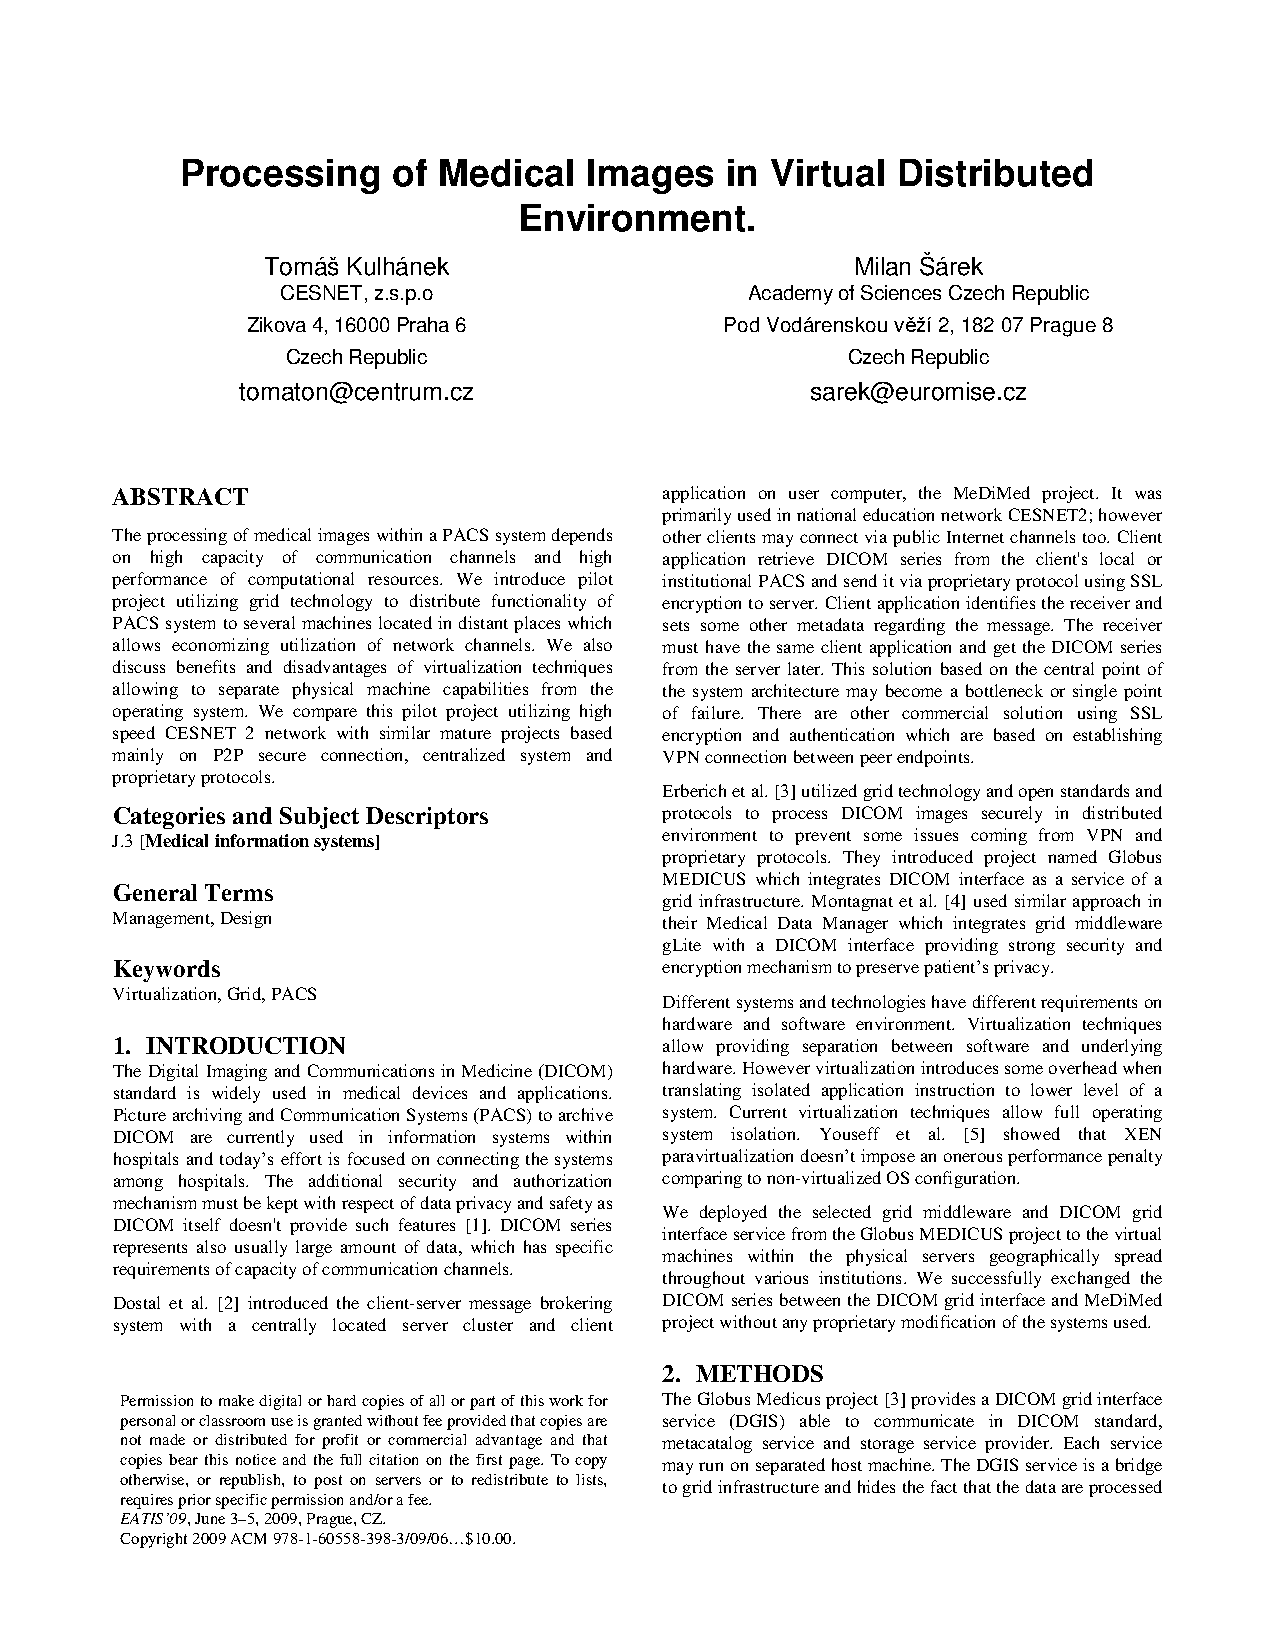
\includepdf[pages=-,pagecommand={\thispagestyle{plain}}]{appendix/a10kulhanek.pdf}
%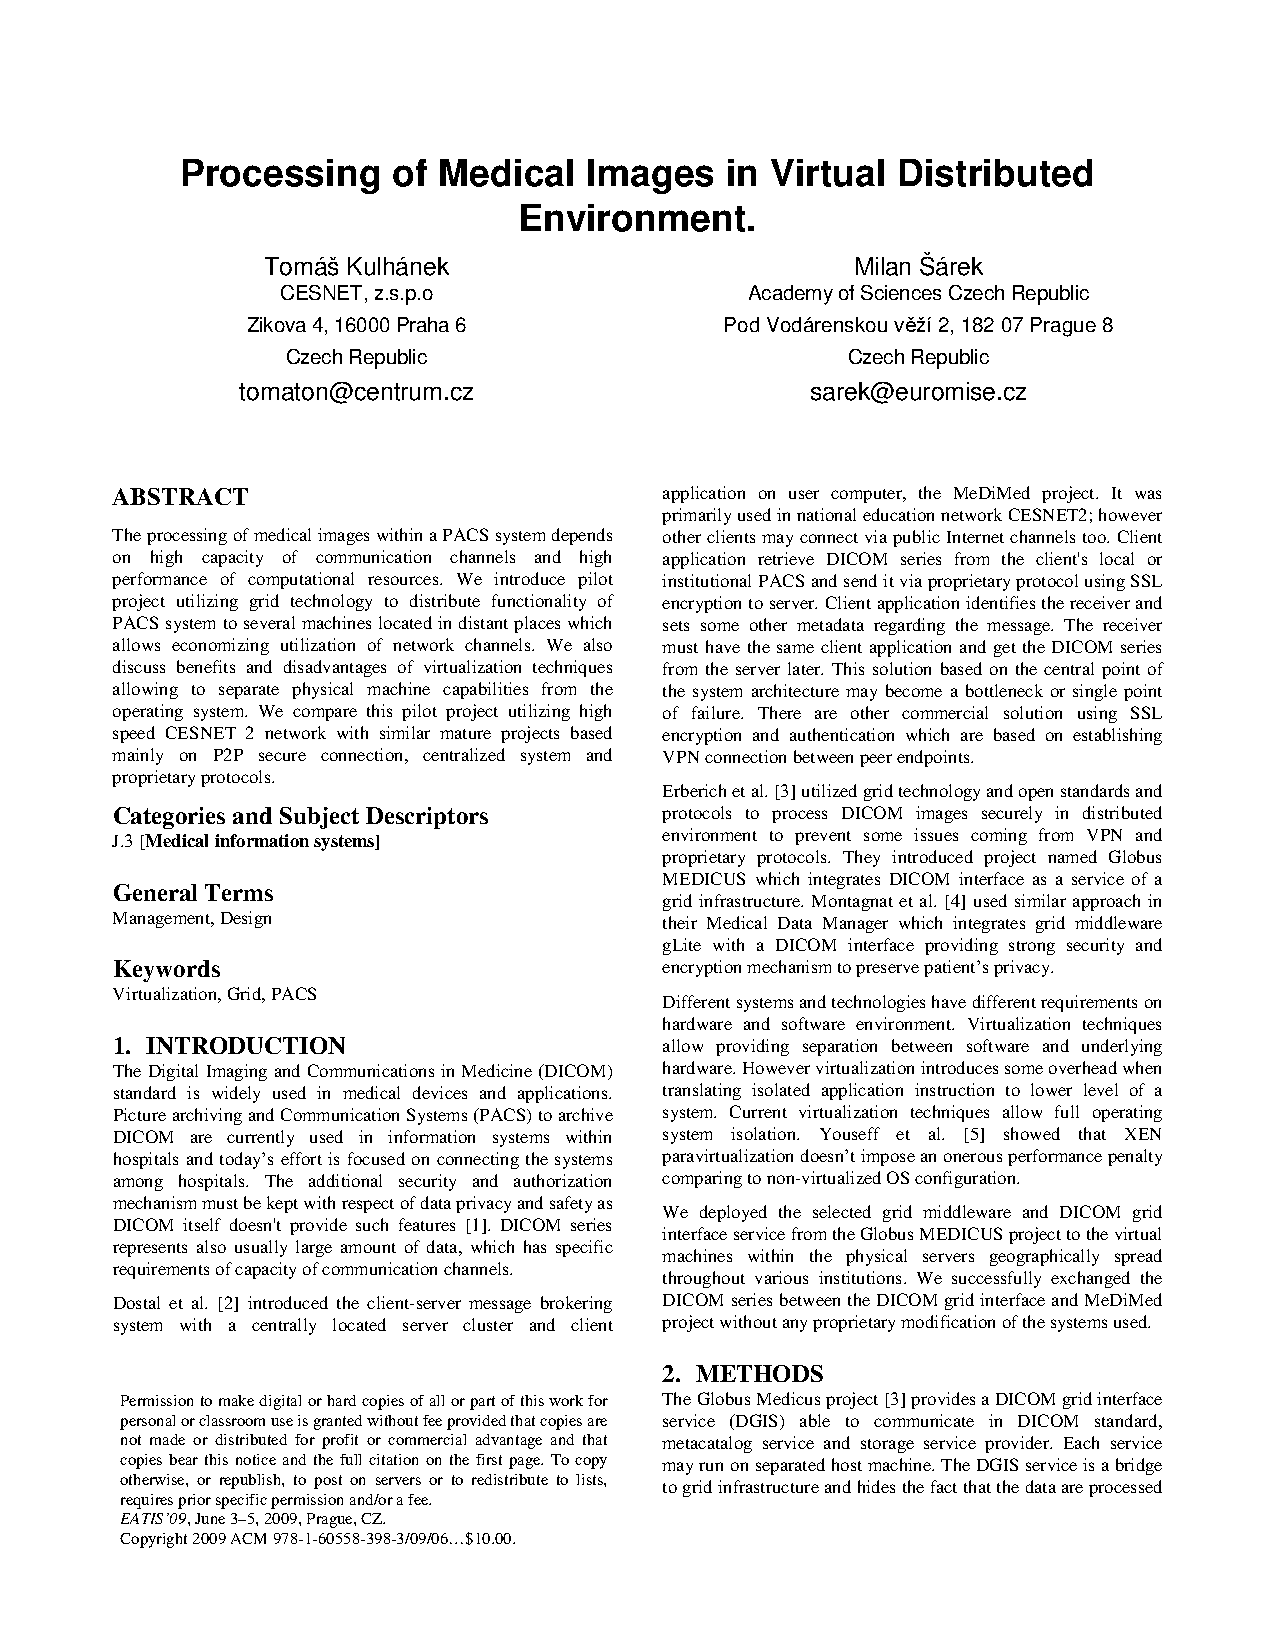
\includepdf[lastpage=3]{appendix/a10kulhanek.pdf}

\chapter{Remote Analysis of Human Voice – Lossless Sound Recording Redirection}\label{app:remote}
The paper \cite{kulhanek2010b} published as
 
\bibentry{kulhanek2010b}

Available online at \href{http://bs2010.biosignal.cz/papers/1092.pdf}{bs2010.biosignal.cz/papers/1092.pdf}.
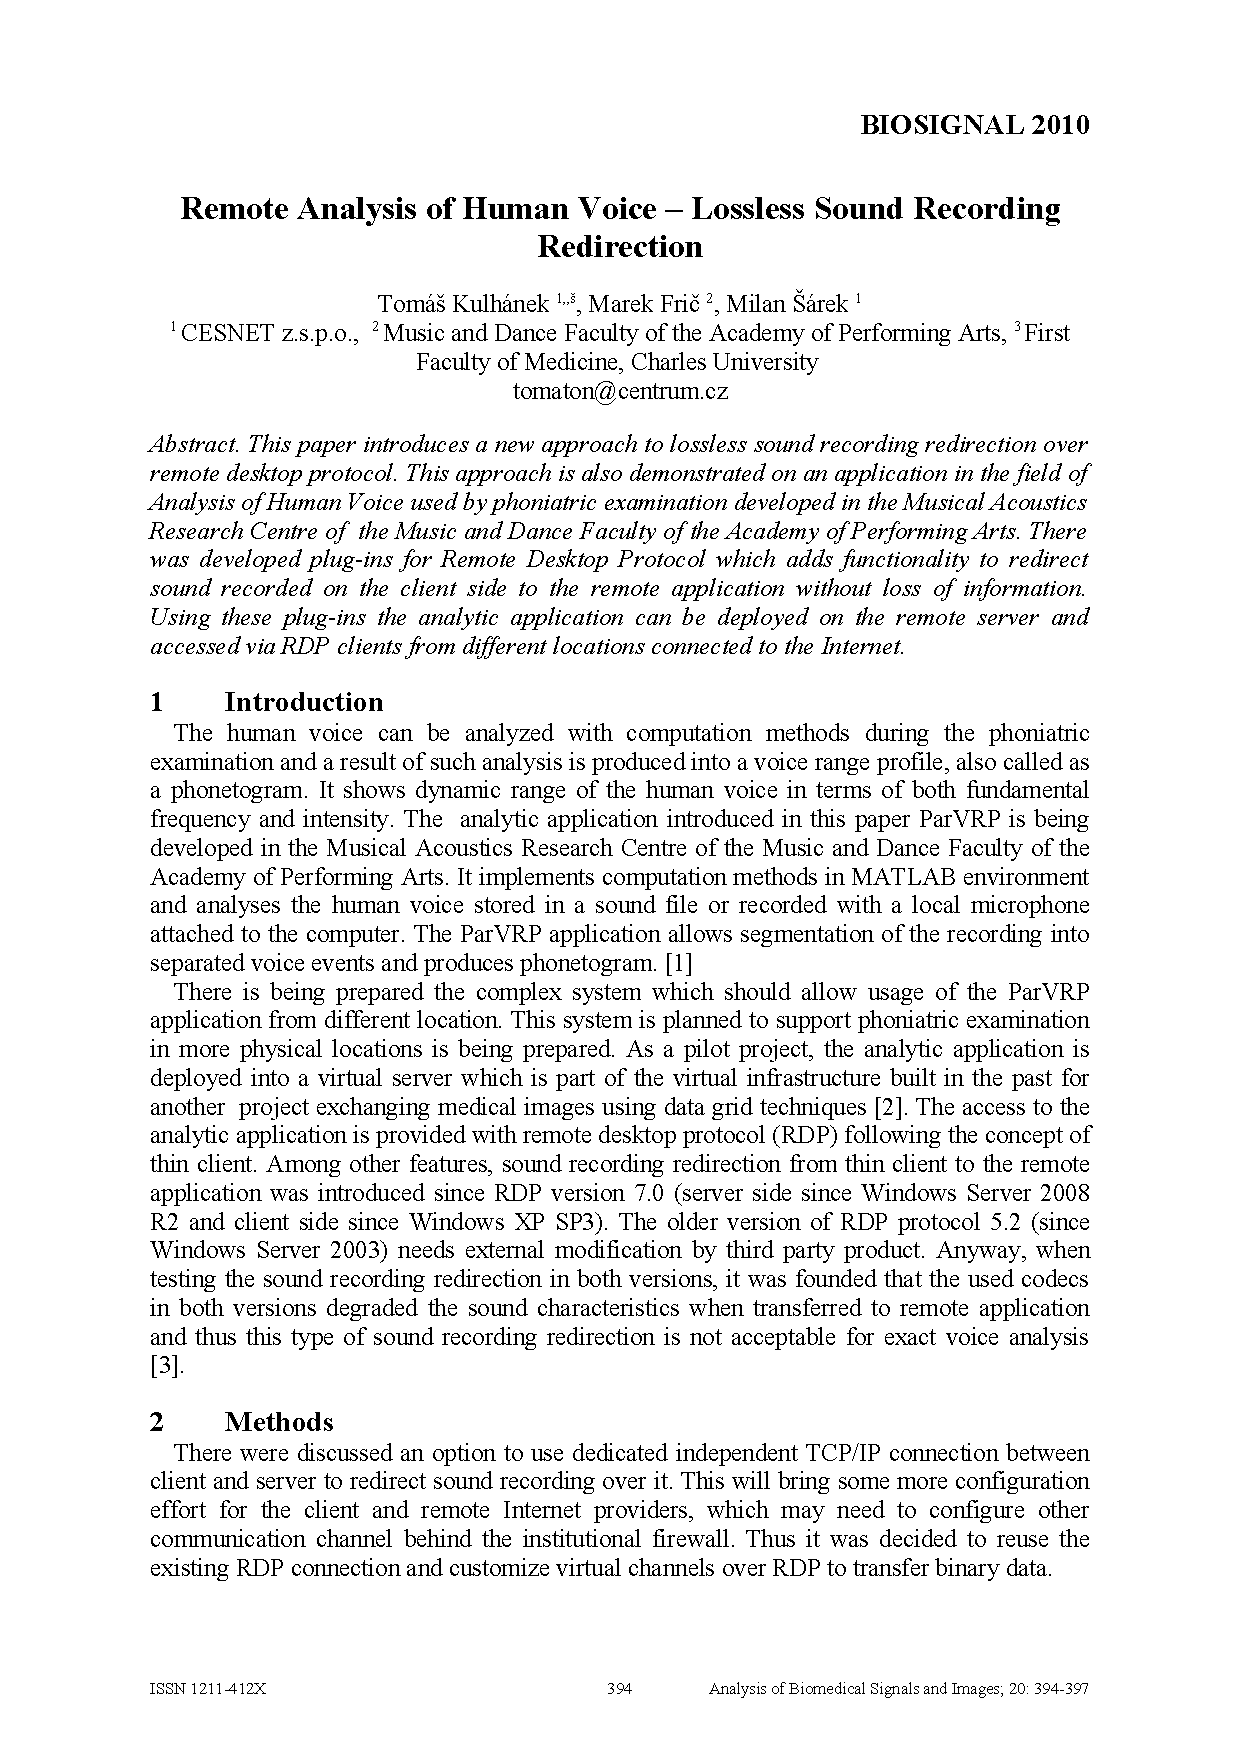
\includepdf[pages={1-4},pagecommand={\thispagestyle{plain}}]{appendix/1092.pdf}
%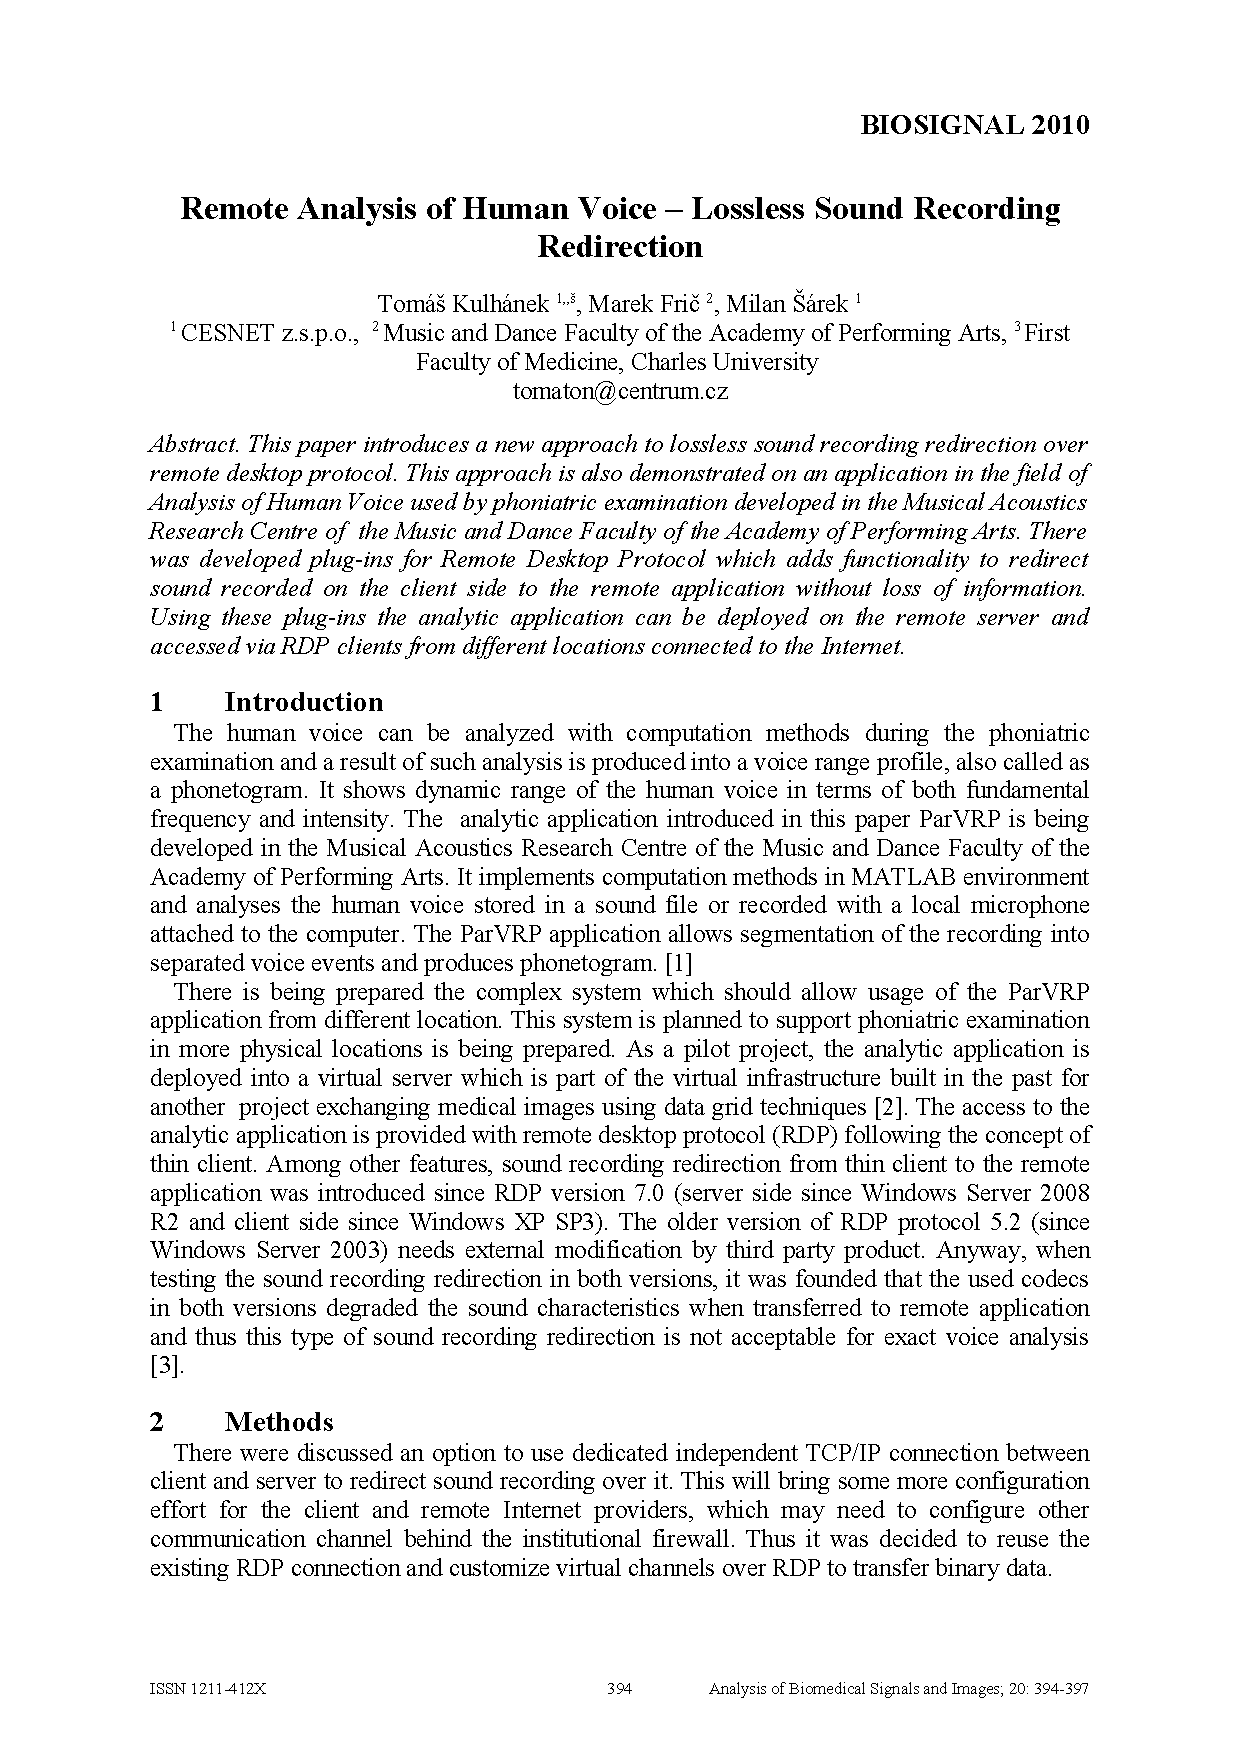
\includepdf[lastpage=4]{appendix/1092.pdf}
%\chapter{From Educational Models Towards Identification of Physiological Systems}\label{app:fromeducational}
The paper \cite{Kulhanek2011} published as
 
\bibentry{Kulhanek2011}

%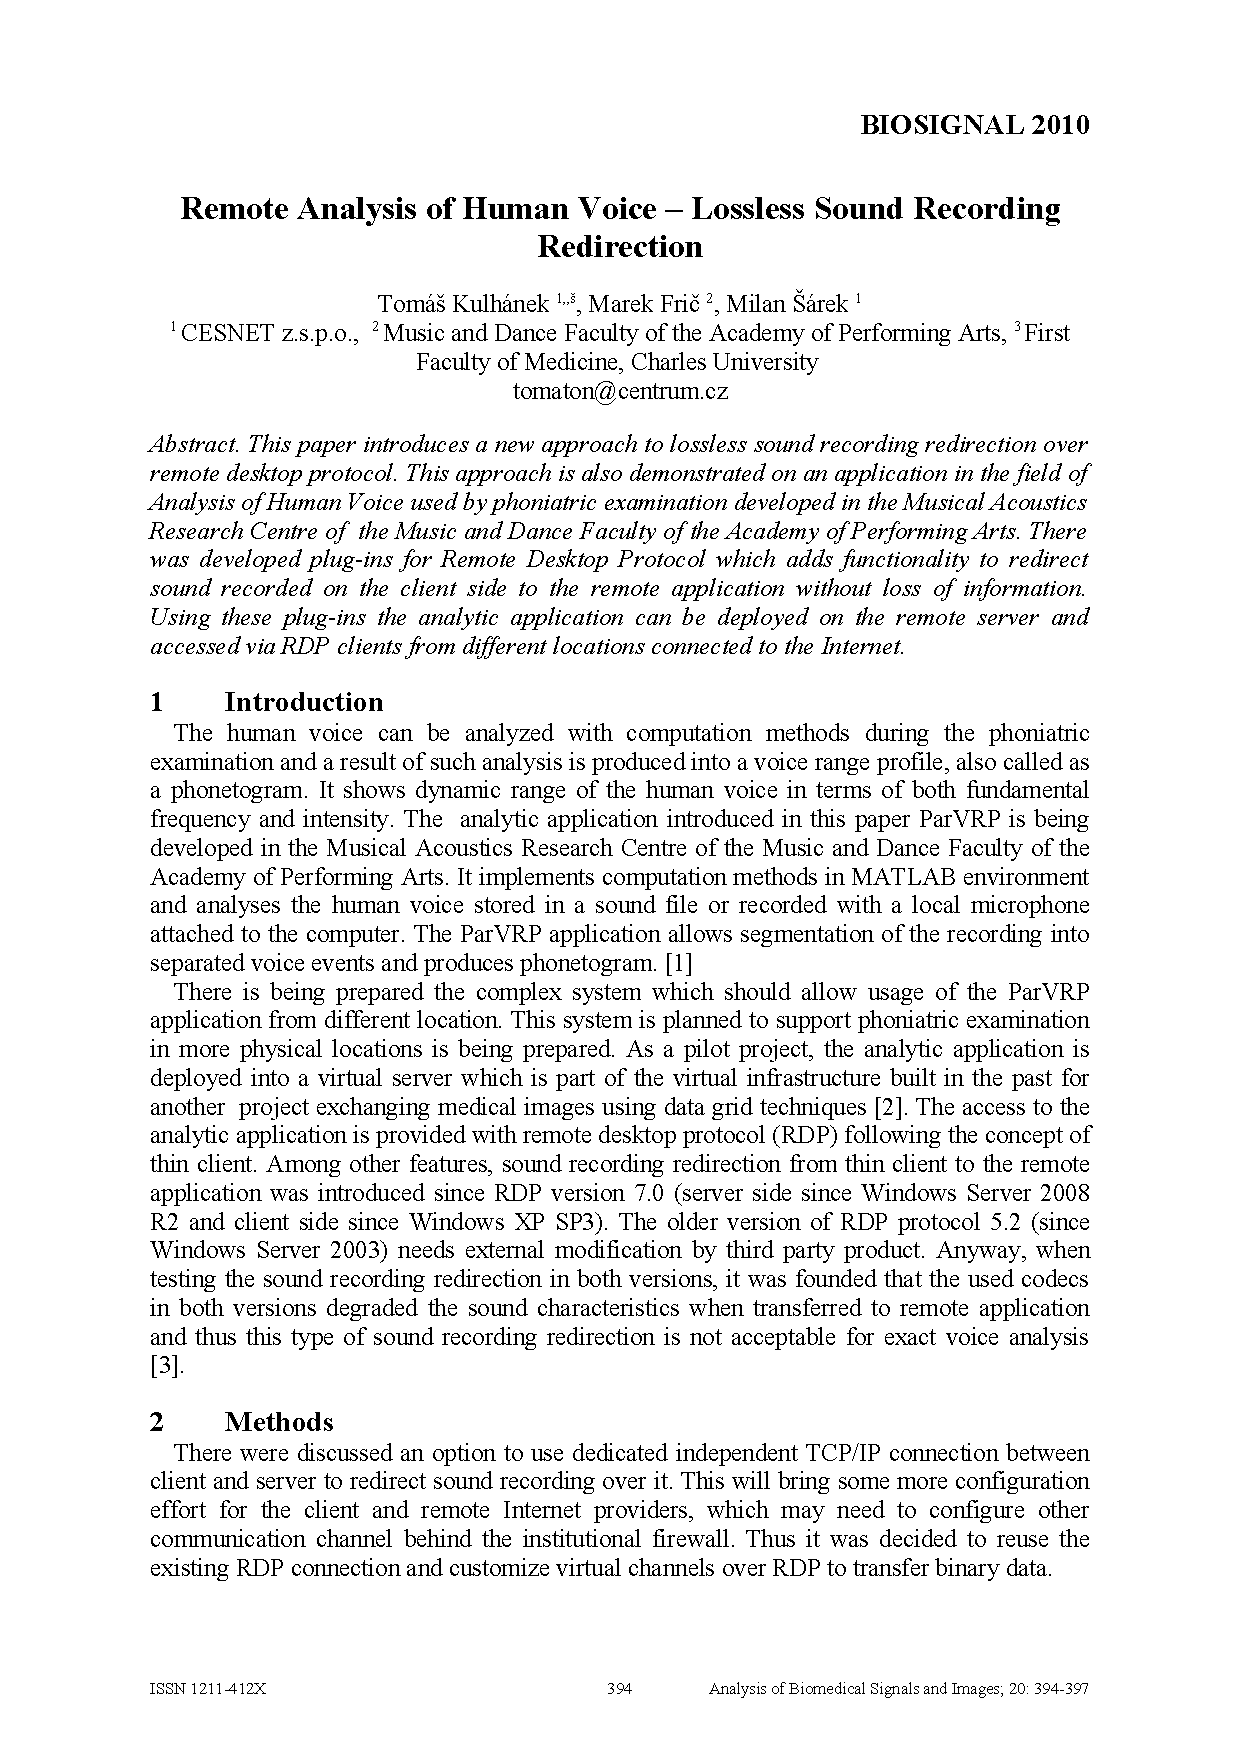
\includepdf[pages={1-4},pagecommand={\thispagestyle{plain}}]{appendix/1092.pdf}
\includepdf[scale=0.9,pages={71-74},pagecommand={\thispagestyle{plain}}]{appendix/mefanet-report-2011.pdf}

\chapter{Infrastructure for Data Storage and Computation in Biomedical Research}\label{app:infrastructure}
The paper \cite{kulhanek2010c} published as
 
\bibentry{kulhanek2010c}

Available online at \href{http://www.ejbi.org/en/ejbi/article/49-en-infrastructure-for-data-storage-and-computation-in-biomedical-research.html}{www.ejbi.org}

The author of this thesis proposed the idea of consolidating and sharing physical resources in order to provide a virtual environment for the specific needs of particular use-cases. The pilot infrastructure was tested on examples of selected research projects.
\includepdf[scale=0.9,pages={61-65},pagecommand={\thispagestyle{plain}}]{appendix/article1.pdf}
%\includepdf[pages={61-65}]{appendix/article1.pdf}
\chapter{Parameter estimation of complex mathematical models of human physiology using remote simulation distributed in scientific cloud}\label{app:parameter}
The paper \cite{Kulhanek2014Parameters} published as
 
\bibentry{Kulhanek2014Parameters}

Available online at \href{http://ieeexplore.ieee.org/xpl/articleDetails.jsp?arnumber=6864463}{ieeexplore.ieee.org/xpl/articleDetails.jsp?arnumber=6864463}

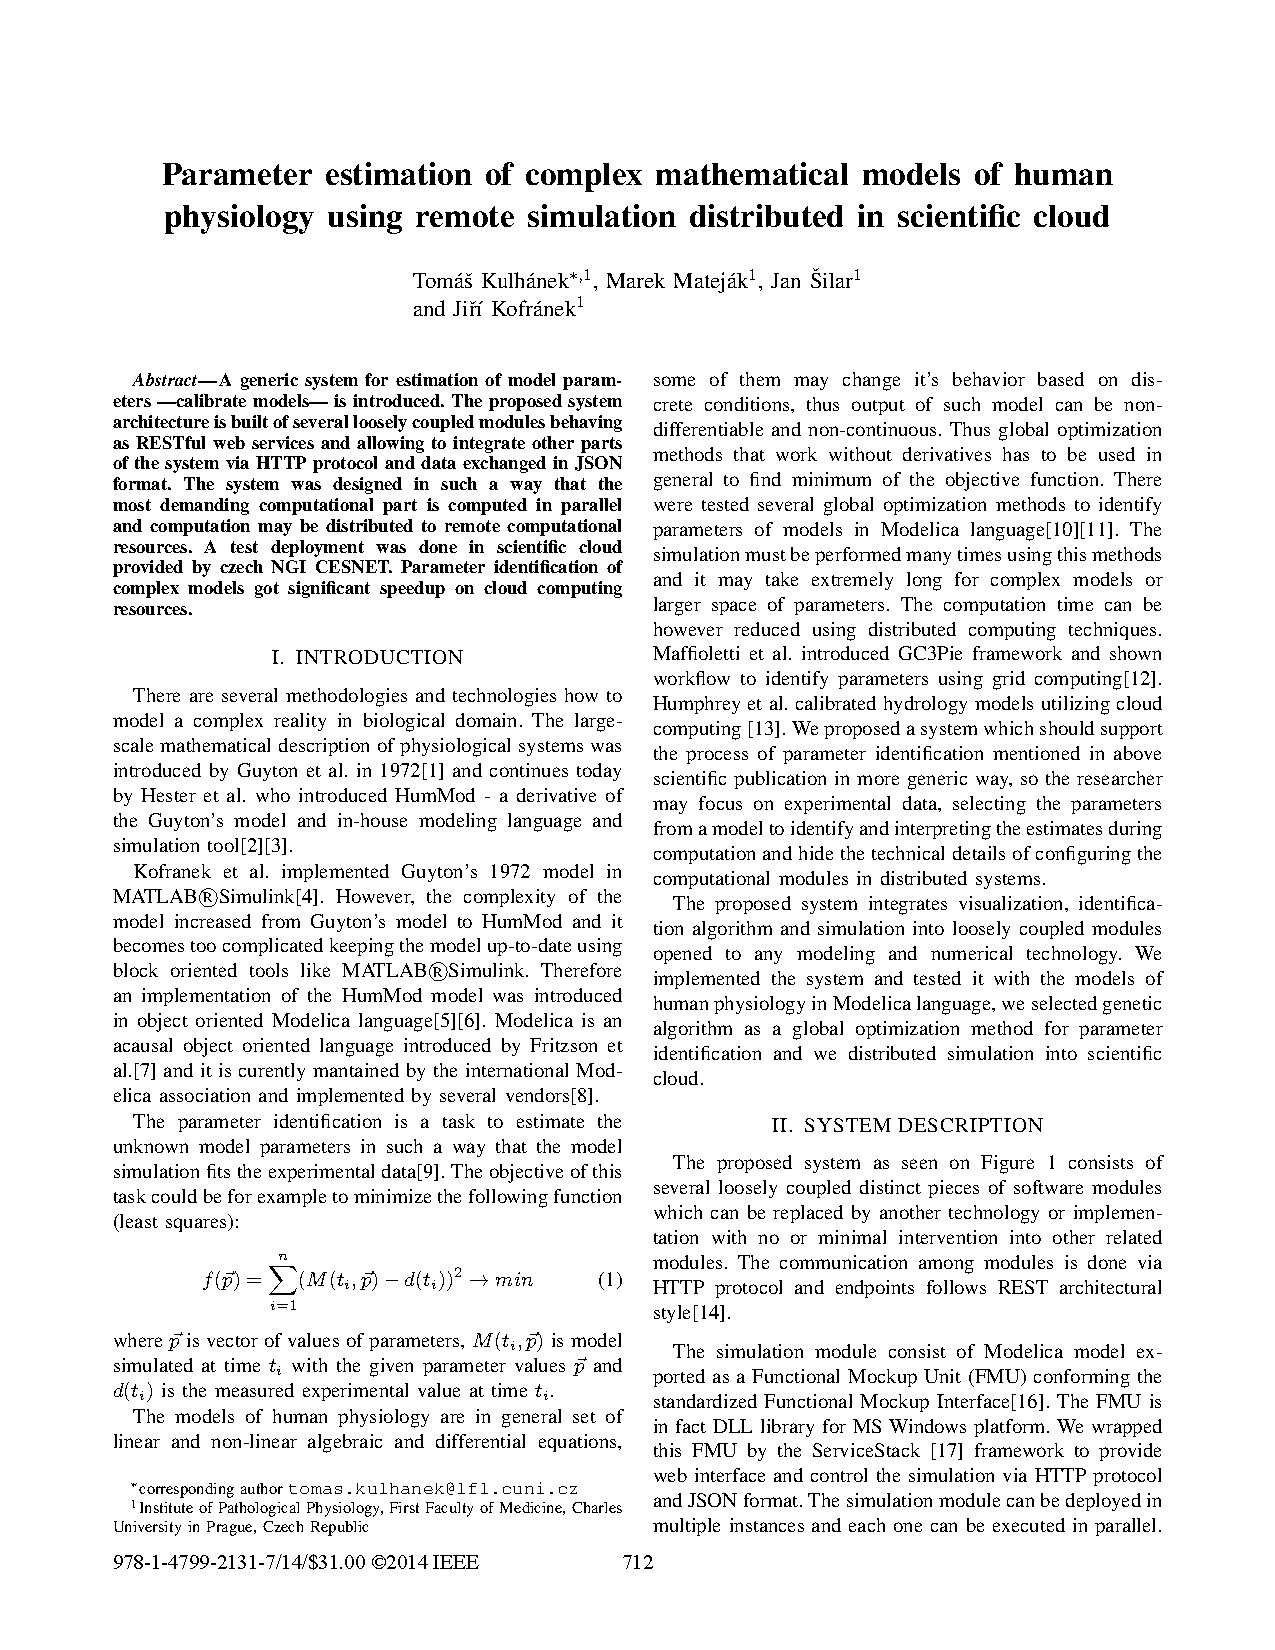
\includepdf[pages={-},pagecommand={\thispagestyle{plain}}]{appendix/06864463.pdf}

\chapter{Modeling of short-term mechanism of arterial pressure control in the cardiovascular system: Object-oriented and acausal approach}\label{app:modeling}
The paper \cite{Kulhanek2014Modeling} published as
 
\bibentry{Kulhanek2014Modeling}

Available online at \url{http://dx.doi.org/10.1016/j.compbiomed.2014.08.025}

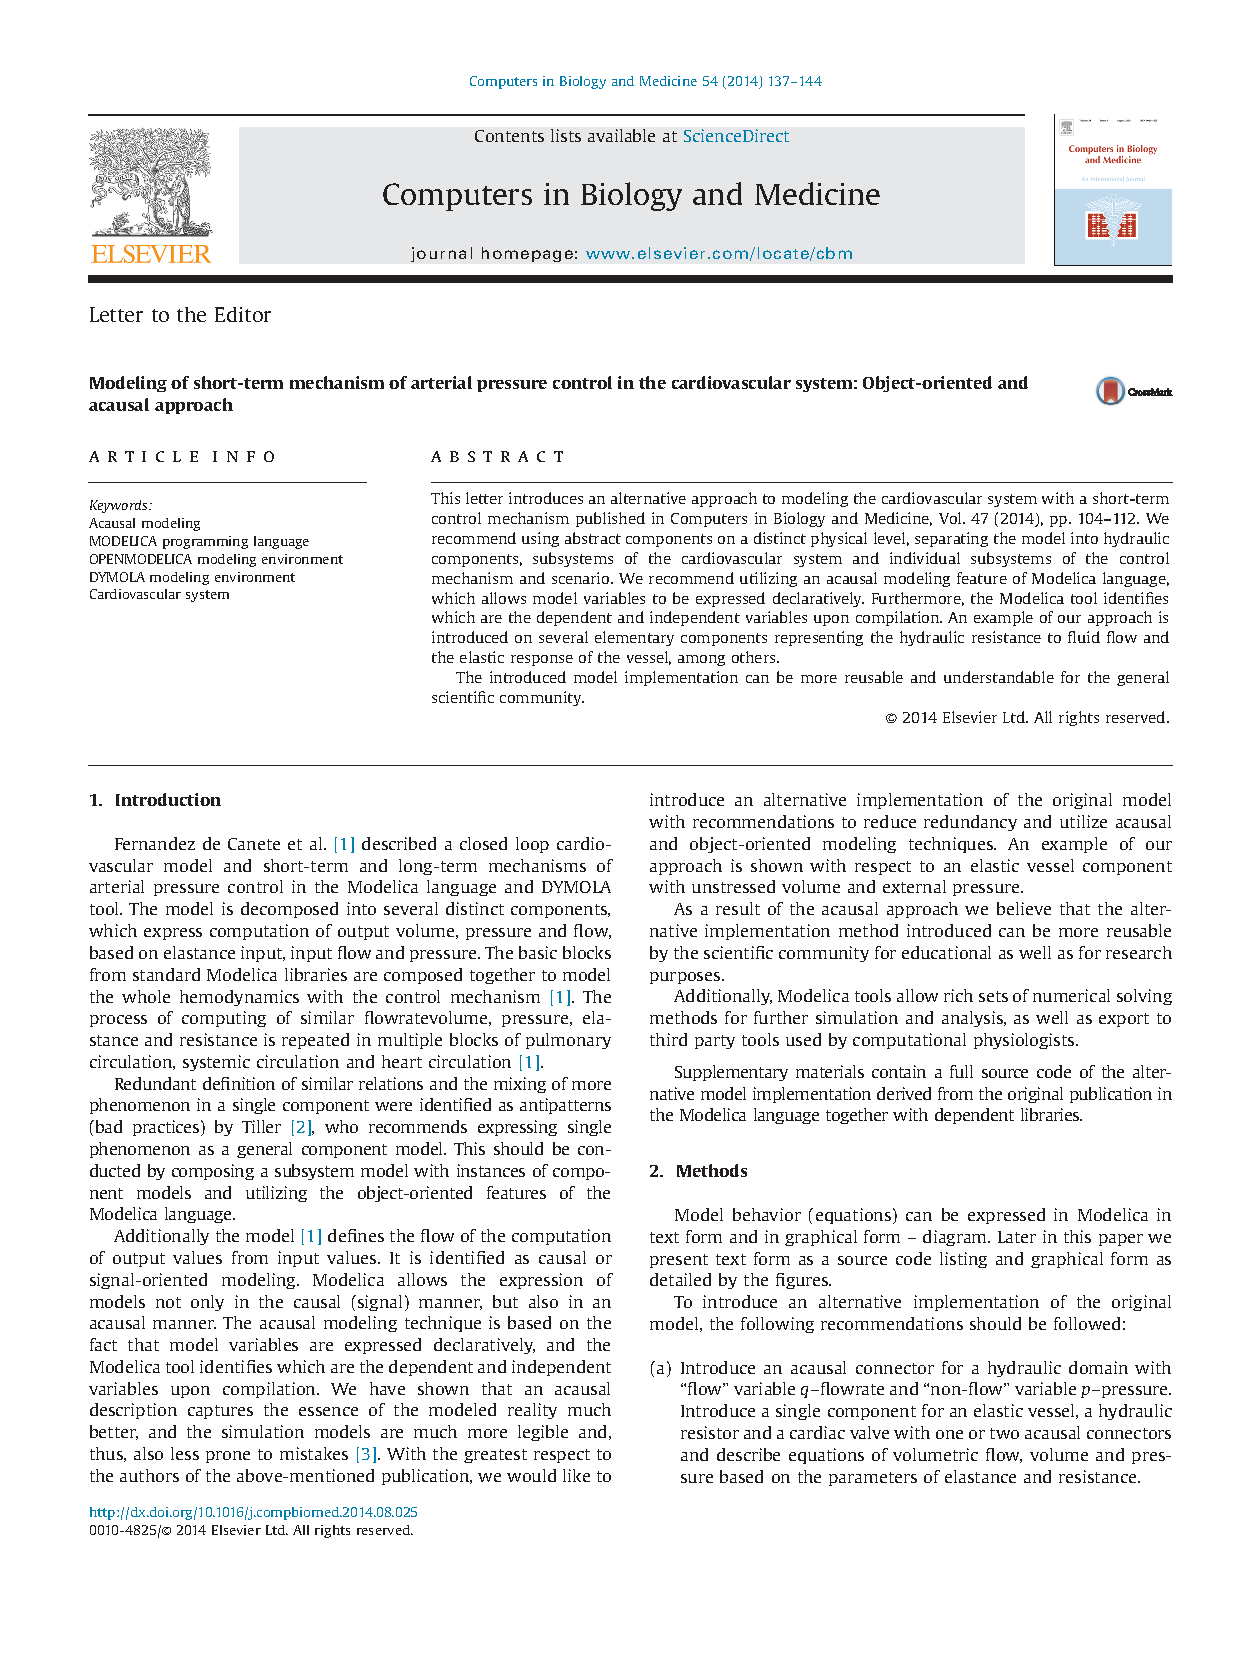
\includepdf[scale=0.9,pages={-},pagecommand={\thispagestyle{plain}}]{appendix/LetterToEditorNew2.pdf}

\chapter{Simple Models of the Cardiovascular System for Educational and Research Purposes}\label{app:simplemodelsd}
The paper \cite{Kulhanek2014mefanet} published as
 
\bibentry{Kulhanek2014mefanet}

Available online at \url{http://mj.mefanet.cz/mj-04140914}

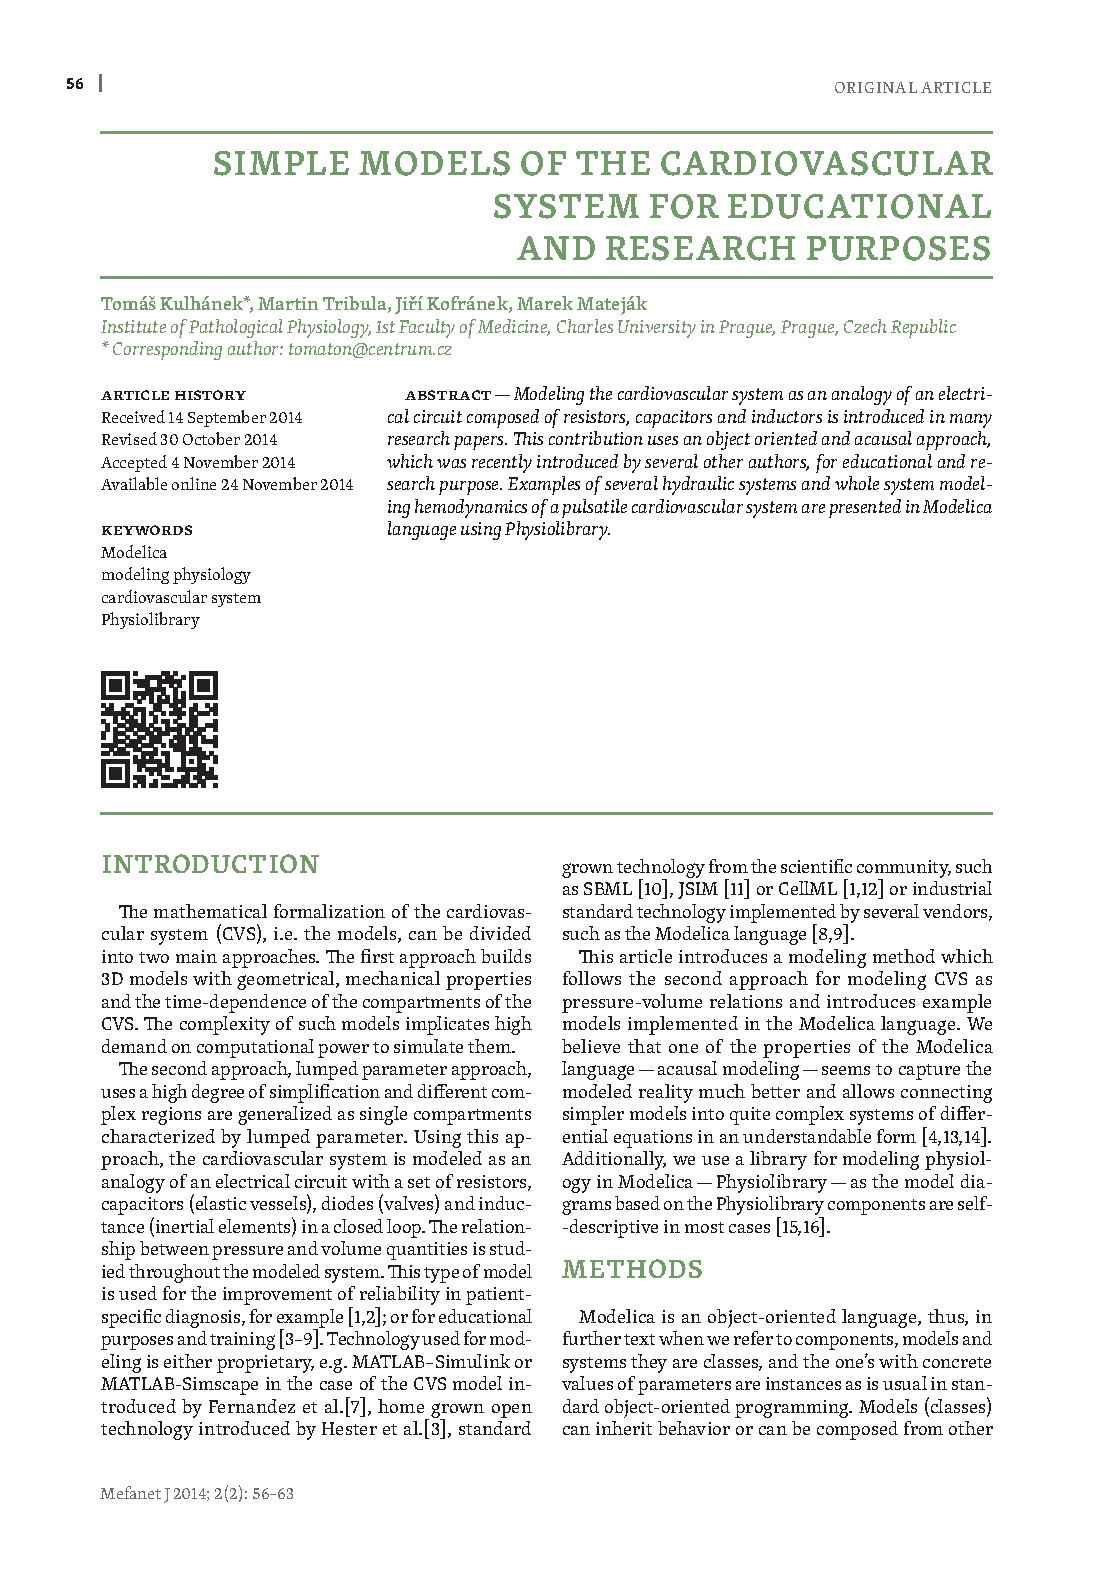
\includepdf[pages={-},pagecommand={\thispagestyle{plain}}]{appendix/mj-04140914.pdf}

\chapter{Adair-Based Hemoglobin Equilibrium with Oxygen, Carbon Dioxide and Hydrogen Ion Activity*}\label{app:adair}
The paper \cite{Matejak2014sj} published as
 
\bibentry{Matejak2014sj}



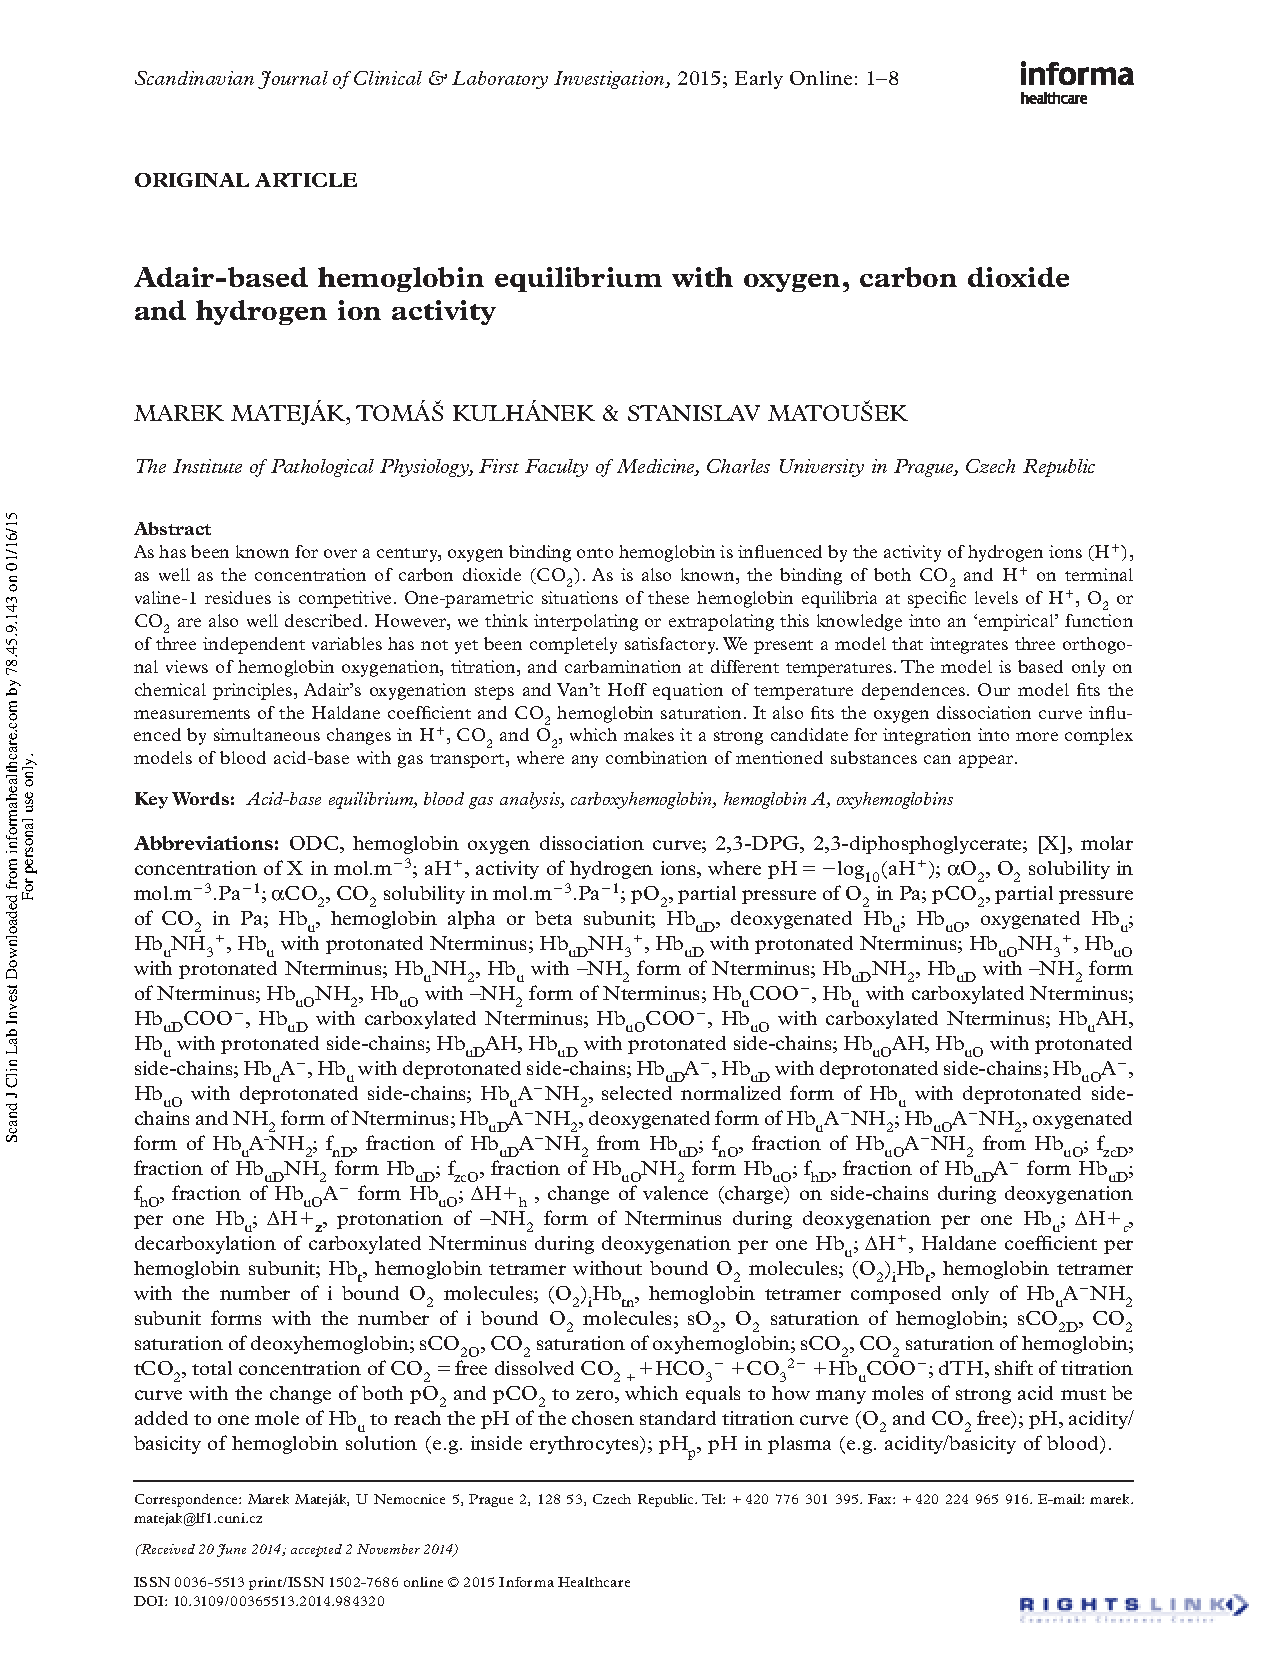
\includepdf[pages={-},pagecommand={\thispagestyle{plain}}]{appendix/sjhemoglobin.pdf}

\end{appendices}
\bibliographystyle{unsrturltom}
\bibliography{bibliography/Dizertace}
\end{document}
